\documentclass[11pt,a4paper,thesis,english]{dcsbook}

\usepackage[utf8]{inputenc}
\usepackage{babel}
\usepackage{listings}
\setcounter{secnumdepth}{4}
\setcounter{tocdepth}{3}

\usepackage{tikz}
\usepackage{pgfplots}
\usepackage{hyperref}
\usepackage{xcolor}
\usepackage{float}
\hypersetup{
    colorlinks,
    colorlinks=false,
    % colorlinks,
    % citecolor=black,
    % filecolor=black,
    % linkcolor=black,
    % urlcolor=black
}

\captionsetup{justification=centering}

\begin{document}

\author{Robert Banaszak}
\title{The use of serverless processing and the FaaS model in web application development}
\supervisor{dr hab.~inż.~Anna Kobusińska}
\date{Poznań, 2021}
\maketitle
\frontmatter

\thispagestyle{empty}\vspace*{\fill}%
\begin{center}Tutaj będzie karta pracy dyplomowej;\\oryginał wstawiamy do wersji dla archiwum PP, w pozostałych kopiach wstawiamy ksero.\end{center}%
\vfill\cleardoublepage%

\tableofcontents{}
\mainmatter

\chapter{Introduction}

\section{Motivation}

\section{Objective and scope of research}

\section{Structure of thesis}

\chapter{Serverless computing} \label{chapter:serverless-computing}

\section{Origins} \label{section:serverless-origins}

The growth of cloud computing significantly influenced the way how server management and server application development are perceived. Around fifteen years ago, most of~the companies were entirely responsible for managing their software, altogether with the~hardware and infrastructure it was running on \cite{RobertsChapin2017}. Around that time, first services capable of outsourcing some part of infrastructure overhead emerged, which started the~idea of~cloud computing.

Amazon Web Services was one of the first service providers that enabled companies to rent computing capacity by announcing the launch of Elastic Compute Cloud (EC2) in~August 2006. It was the first Infrastructure as a Service (IaaS) product on the market that allowed companies to run their server applications on Amazon's machines that are~billed per usage time and are available within minutes from requesting new resources.

Leveraging such a service model brings a handful of benefits. It reduces the labour cost by outsourcing hardware management to the provider and infrastructure cost by paying based on actual usage of services. Furthermore, it enables companies to scale the number and type of servers in correlation with the traffic and demand for processing. Finally, it~encourages testing new solutions developed by companies and decrease the lead time, by~making the required infrastructure available within minutes instead of months, utilising favourable billing flexibility.

The cost of IaaS solutions is profitable to providers, because of technical improvements done in terms of hardware virtualization and the economy of scale on which they operate. Shortly after, other vendors such as Microsoft, Google and DigitalOcean embraced the notion of public cloud by providing services and resources from their own data centers. At~the~same time, tools like Open Stack enabled companies to use hardware from their own data centers in the same way, forming the idea of private cloud.

The next step in the cloud evolution is Platform as a Service (PaaS). As~a~layer on~top of IaaS, it adds operating system to the outsourced infrastructure stack, enabling to~deploy the application code directly. In that model, the platform takes responsibility for~managing the operating system as well as monitoring and running the application. Google App Engine, AWS Elastic Beanstalk and Heroku platform can be distinguished as most popular PaaS solutions, while one of the most frequently mentioned self-hosted variant is~Cloud Foundry.

The growth of containerisation technologies introduced another type of service called Container as a Service. Technologies like Docker allowed developers and system administrators to deliberate more clearly on the application requirements and separate it from the~operating system. Solutions such as Marathon, running on top of Mesos, and Kubernetes introduced a possibility to manage and orchestrate containers on self-hosted machines. The services provided by cloud vendors include for example Google's Compute Engine or~Amazon's Elastic Container Service (ECS) or AWS Fargate. With the growing popularity of Kubernetes, dedicated services leveraging that platform emerged, including Amazon Elastic Kubernetes Service (EKS) and Google Kubernetes Engine (GKE).

Each of the described services are next generations of infrastructure outsourcing, which raise the level of abstraction from the development perspective and hand off more and more responsibility related to infrastructure management to the cloud vendor. Despite the fact, for each of the mentioned services the smallest unit of processing is some sort of server application or running application process in the virtual machine or within the container.

Serverless is considered as a next step in the cloud computing progression. The term serverless was one of the first used by Ken Fromm in his paper \cite{KenFromm}. It describes the~notion of architecture migration from monolithic applications running on servers into distributed systems that consist of multiple components, processes and data stores with the goal to perform various tasks and process numerous flows. The serverless architecture enables developers to make a mind shift accordingly. Computing resources can be used as services, which makes it possible to shift thinking from the servers level to the tasks level, taking away the complexity of infrastructure management. The servers are still used underneath, but developers don't need to worry about managing them any longer.

Such an architecture model was leveraged firstly by mobile applications built on top of hosted database solutions, such as Parse (later acquired by Facebook) and Firebase around 2012 (obtained by Google). Nonetheless, the most significant event shaping the serverless architecture was the announcement of AWS Lambda in 2014, altogether with the introduction of API Gateway in 2015. By the middle of 2016, major cloud vendors such as Microsoft and Google embraced the serverless architecture approach and started offering their services for developing serverless applications.

\section{Defining serverless} \label{section:serverless-definition}

Despite the fact that the idea of serverless computing emerged about a decade ago, it~has~been already widely adopted by leading cloud providers. Currently it covers a~range of~technologies, components and cloud services. Nevertheless, there is no clear and concise view on what ''serverless'' is. Various vendors, organisations and research groups tried to~define what the serverless term means for them.

Cloud Native Computing Foundation is the organization working towards standardisation of numerous cloud-related technologies and components. It maintains a sustainable ecosystem for cloud native software by bringing together and collaborating with various members of the cloud community. According to ''CNCF Serverless Whitepaper'' \cite{CNCFServerless}.

\begin{quotation}
Serverless computing refers to the concept of building and running applications that do not require server management. It describes a finer-grained deployment model where applications, bundled as one or more functions, are~uploaded to a platform and then executed, scaled, and billed in response to~the~exact demand needed at the moment.
\end{quotation}

Another definition considering the serverless service capabilities can be found in~a~booklet made by Mike Roberts and John Chapin titled ''What is Serverless?'' \cite{RobertsChapin2017}.

\begin{quotation}
\noindent A Serverless service:
\begin{itemize}
    \item Does not require managing a long-lived host or application instance
    \item Self auto-scales and auto-provisions, dependent on load
    \item Has costs that are based on precise usage, up from and down to zero usage
    \item Has performance capabilities defined in terms other than host size/count
    \item Has implicit high availability
\end{itemize}
\end{quotation}

The cited definitions contain insightful information about features of serverless architecture and capabilities of its components. These can be summarized as follows:

\begin{itemize}
    \item Serverless architecture defines the new model of~developing and executing workloads. The application consists of multiple serverless components configured together to run the business logic within the application code, designed to be executed in a serverless environment.
    \item It does not require to maintain, provision and monitor servers and applications. Serverless does not mean that there are no servers --- the overhead of managing them is handed off to the cloud provider.
    \item Deployment model is more granular. Having the application built from multiple components configured to work together, the deployment can update only selected ones.
    \item Platform is responsible for provisioning and executing the applications. With a large resource pool maintained by cloud provider and the possibility to quickly allocate it, the solution can be scaled automatically to the current load requirement almost instantly.
    \item The cost is proportional to the resource usage. Each of the components involved in performing the computation is billed granularly, with an accuracy to hundreds of~milliseconds or number of executed operations, with no cost when being idle. Executing hundred operations in parallel will cost the same amount of money as~running that workload sequentially.
    \item The performance is not related to the host size. Some of the cloud providers enable customers to choose how much memory and CPU can be allocated for the environment. Nevertheless, the configuration is abstracted from the capabilities of the underlying machine that is used as an execution environment.
    \item The serverless components are built with high-availability and fault-tolerance in~mind. Despite the fact that developers are no longer concerned with servers, the underlying vendor's machines can still fail. When using serverless services we expect that cloud vendors will provide transparent high availability for its services. Although, as developers it may be necessary to handle consequences of some errors and failure occurrences properly.
\end{itemize}

\section{Serverless components} \label{section:serverless-components}

When considering the serverless architecture, it refers to a range of technologies provided by cloud platforms. Two different areas can be distinguished, defining two distinctive components:

\begin{itemize}
    \item \textbf{Backend as a Service} refers to third party services or generic components, capable of replacing some part of a server side application, that was previously developed internally or self-provisioned. It exposes an API which allows for integrating the component with the rest of the application.
    \item \textbf{Function as a Service} is an event-driven execution environment for running application code within stateless and ephemeral containers with strictly limited execution time.
\end{itemize}

Aforementioned components used simultaneously enable developers to build fully-fledged solutions utilising serverless architecture and are offered together within a single cloud platform.
Even though presented areas serve different roles, they share common features and capabilities. These could be listed as follows:

\begin{itemize}
    \item Require no resource management and are entirely provisioned by cloud provider
    \item Utilise the event-driven model for processing
    \item Underlying platform ensures automatic horizontal scaling, high availability and fault tolerance
    \item Billing is proportional to actual usage
\end{itemize}

\subsection{Backend as a Service}

The concept of Backend as a Service (BaaS) gathers various domain-generic, repeatable application components capable of replacing some part of application logic or providing some functionalities. They can be accessed and integrated into developed applications through API defined by its provider.

Taking into consideration most popular requirements of various applications, the majority of them need to store and manage the data. Depending on the requirements, the~information should be stored in a structural way in databases or can be stored regardless of their shape in file storage service. For teams developing mobile or web applications it~is~convenient to rely on some third party components to store and access the data directly from the application. Services like Google's Firebase meet such requirements and give access to the database entirely managed by a cloud vendor. Depending on the complexity of developed product, it may be required to incorporate some more advanced components to process required tasks or flows, reflecting the business logic of application. Mechanisms serving as notification services, exposing some publish-subscribe capabilities for defined events, could be applicable in that case. It is essential to notice that such components are replacing previously self-hosted components such as databases or other data stores, message brokers or similar services responsible for processing data streams incoming from various sources.

Looking closer from the application logic point of view, there are also repeatable functionality implementations that can be extracted and reused across multiple developed applications. Majority of the products will require some features enabling users to manage their identity and associated permissions. Most of the time, the capabilities will be~not only limited to registering and logging users, but it will also include integrations with other services as identity providers. Managing and sending emails can be considered as another functionality that can be extracted into separate component from the code perspective and reused in other applications. Products such as Auth0 (serving as fully featured authorization and user management service) or Mailgun (capable of managing and processing emails) makes it possible to replace entirely the repeatable part of business logic.

Specific components and services that can be classified as Backend as a Services will be~covered in more details in chapter \ref{chapter:serverless-service-providers}, when analysing services provided by leading cloud vendors. All of the mentioned components enable developers to create fully fledged applications and services similar to the solutions built using self-hosted component equivalents. The difference for given components is the fact that they characterise by capabilities of~the~serverless architecture. They are provided by cloud vendors, who take responsibility for managing, provisioning and scaling them depending on the demand. Moreover, the~possibility to replace the repeatable application features by utilising third party services enables developers to iterate faster and shorten the lead time.

\subsection{Function as a Service} \label{chapter:serverless-faas}

The second area refers to Function as a Service (FaaS) that serves as an environment for~executing application code. It introduces a new architectural approach in terms of~developing, structuring and deploying the application logic, which is oriented towards individual tasks and operations.

Mike Roberts briefly described the idea of FaaS \cite{MartinFowlerServerless} based on the definition of~AWS Lambda \cite{AWSLambda}, which is currently one of the most commonly used implementation of~a~Function as a Service model. Based on his summary several main features of FaaS can be~highlighted:

\begin{itemize}
    \item The main idea of FaaS is to run application code without managing servers and application processes. It is a common feature with other approaches like CaaS or PaaS, where the responsibility for managing applications is placed on the cloud vendor. However, the key difference with FaaS is the fact that the function execution time is strictly limited in contrast to long-lived processes existing in aforementioned services.
    \item The functions are invoked and executed on the underlying platform in response to~specific events occurring or coming in the system. Based on that cloud provider handles resource allocation and runs the function code in an ephemeral container, created based on runtime needs. These are destroyed shortly after the event is~processed by the application logic in the function. Together with limited execution time it is a significant architectural restriction for the FaaS model.
    \item Given the fine-grained execution model, horizontal scaling can be easily and automatically handled by the cloud provider. When there is an increased traffic in the system, the platform responsible for executing functions allocates resources to create and run more functions, which will be capable of processing the increased traffic. An~analogous situation takes place when there is no traffic, therefore there is no need to allocate resources for running functions code.
    \item As a consequence of greater granularity of the application code and managing the function execution by cloud provider, the deployment process differs from the traditional system. Each function can be independently packed and uploaded to the FaaS platform, which takes responsibility for executing it.
    \item Most of the cloud platforms do not require to use neither predefined framework nor programming language. Although cloud providers define the list of environments and languages that are supported by the platform, any process that is bundled into the artifact and can be executed from it, is capable of processing the incoming event.
\end{itemize}

Selected aspects of Function as a Service architecture are covered in more details based on ''CNCF Serverless'' whitepaper \cite{CNCFServerless} in the following sections.

\subsubsection{Function lifecycle}

Before analyzing the execution model in more details, it is important to examine the~deployment process accompanying the development of a function. Alongside with providing the function code, the developer is responsible for specifying one or more events upon which function will be triggered. Additionally, metadata defining for example the function version, environmental variables, execution role and other configuration parameters can~be~defined. The function and specification prepared in that way is uploaded to~the~cloud~provider and processed by a dedicated builder entity, resulting with a function artifact (depending on the cloud platform and selected runtime it can be a binary file, container image or a package). Next, it is deployed on a cluster managed by a FaaS controller responsible for provisioning, controlling and monitoring function instances based on incoming events.

\begin{figure}[h]
    \centering
    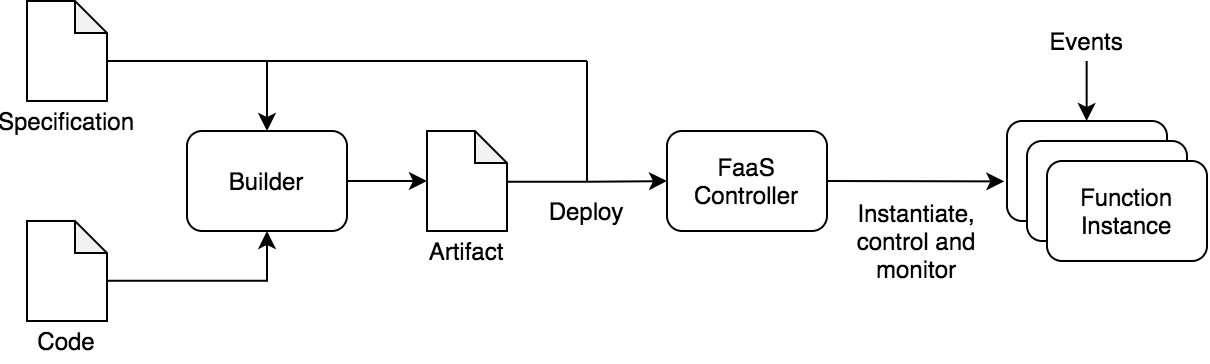
\includegraphics[width=0.8\textwidth]{assets/02-serverless/ServerlessDeployment.png}
    \caption{Function deployment and invocation process}
    \label{fig:function-deployment-and-invocation-process}
\end{figure}

Furthermore, the serverless platform may provide additional actions related to~the~function management such as executing, publishing, updating and deleting the function or~its metadata. Also, a particular version of the function can be labeled or aliased, which can come in handy when operating the serverless system on a larger scale. Logs and~statistics are gathered alongside function execution.

The function is executed in an event-driven model and within strictly limited processing duration. The whole process begins when an event triggering a particular function is~dispatched. It is detected and registered by an underlying serverless platform. The~controller, responsible for managing function executions, looks for functions associated with incoming events, gets their code and configuration and allocates an adequate amount of~resources from the managed resource pool. The~new~execution environment is created inside a lightweight, ephemeral container and language runtime for the function is bootstrapped. When the environment is ready, the triggering event is redirected and processed by~the~application logic included in the function code.

The results of computing are sent back to the event dispatcher. Meanwhile, the function can create new events during its execution. The computing duration is limited by~the~majority of service providers up to a few minutes, after that the computation is~completed with timeout. Finally, the lightweight container including the execution environment is~destroyed.

Most of the providers delay the container deletion for longer than a couple of minutes due to optimisation related with reusing the same container instance when the next event occurs in the system. Reusing an already initialised execution environment is called a~''warm~start'' and allows to reduce the startup latency related to resource allocation and runtime bootstrap. The opposite situation takes place when the new container instance needs to be initialised and the host process needs to be created. Most of the time it~requires additional time, impacting the request processing duration and it is called a~''cold~start''.

\begin{figure}[h]
    \centering
    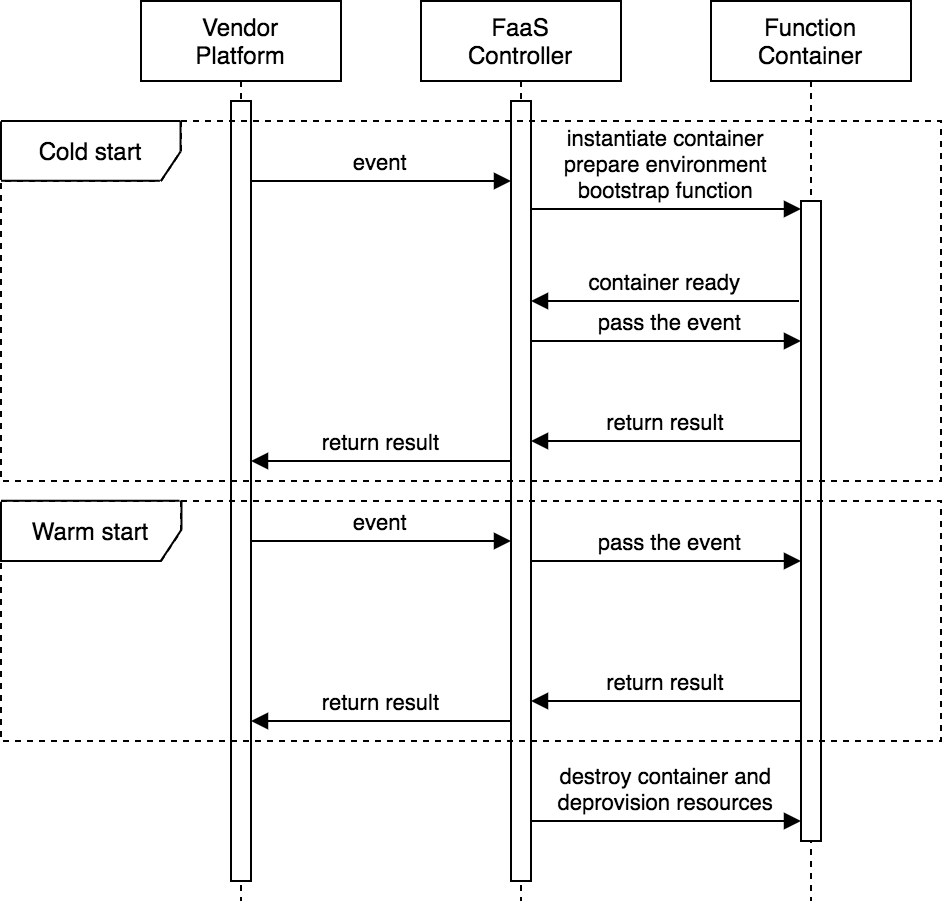
\includegraphics[width=0.7\textwidth]{assets/02-serverless/ServerlessExecution.png}
    \caption{Function execution process considering ''cold~start'' and ''warm~start''}
    \label{fig:function-execution-process}
\end{figure}


\subsubsection{Function environment} \label{section:serverless-function-environment}

The characteristic of the function environment has been already drafted during description of the function lifecycle. Due to improvements in the software virtualisation field, cloud vendors can benefit from efficient and elastic management of large resource pools. It~enables vendors to allocate lightweight and ephemeral containers efficiently, serving as~an~execution environment. Each of them is initialised to executes code of one of~the~functions at a time and it is destroyed shortly after, releasing the resources to the common resource pool. Even though containers can be reused for the optimisation purposes when handling subsequent events occurring in the system, it~is~not~guaranteed by the~serverless platform and should not be taken for granted by developers, that some data will be~preserved for~subsequent invocation.

Such an architecture leveraging stateless containers allows for automatic horizontal scaling. When multiple concurrent events occur within the system, the platform is capable of creating a separate container to process each of them independently. In order to handle spikes of traffic effectively, quick provisioning of the containers and reducing their startup latency is required and it is a purpose of many research works and improvements made by both researchers and cloud vendors

As mentioned before, ephemeral containers are dismissed shortly after the execution alongside with their internal state. For some types of computing it would be desirable to~preserve that state. To address that issue, external components need to be involved to~persist the data. Nevertheless, it introduces the need to communicate with some external service and it is often associated with additional delays resulting from the communication overhead.

\subsubsection{Function invocation} \label{section:serverless-function-invocation}

The serverless architecture utilises an event-driven processing model. The developer's task is to define the configuration that maps events coming to the system with appropriate functions. Each of dispatched events can trigger one or more functions as well as each function can be invoked by one or more predefined events --- there is a many-to-many association between functions and event sources. The mapping can also refer to a particular version of the function or alias, which can greatly simplify the~deployment process by replacing the function code for a given alias without modifying the configuration.

Various data sources can~be~divided into several categories, distinguishing among the~others:

\begin{itemize}
    \item Endpoint Services - Most of the time associated with API Gateway components, which introduces mapping between request coming from APIs (such as REST or~WebSocket) and associate them with corresponding functions.
    \item Storage Services - Category includes numerous BaaS components provided by a cloud vendor like databases, file storage or cache services. Events can be emitted based on~operations performed on the data such as creation, deletion or modification~of~it.
    \item Messaging Services - Services providing mechanisms for data streaming, message brokers or various services sending notifications.
    \item Scheduled events - That category includes services capable of emitting events periodically at a given time or at a selected interval
\end{itemize}

Based on the use case, several invocation types can be differentiated:

\begin{itemize}
    \item Synchronous Request - Includes cases when the client sends a request and waits for~the~response. It is used most frequently for HTTP requests.
    \item Asynchronous Message Queue Requests - Refers to events emitted from various data sources, when messages are published to some exchange that later distributes them to other subscribers. Messages are delivered exactly once without strict ordering.
    \item Event Streams - Are based on streams of messages, logs or files. Sequence of record is most of the time partitioned into several shards.
    \item Batch Jobs - Refers to jobs that can be split into smaller tasks and processed in~parallel by multiple functions. The entire process is completed when all subsequent tasks are finished.
\end{itemize}

\section{Benefits and challenges} \label{chapter:serverless-benefits-and-challenges}

The emergence of serverless architecture has met with great interest from various software architects, developers and companies that noticed numerous advantages of this approach. In addition to the promise of significant cost reduction, the development and operational opportunities and reducing time to market are just a few of the benefits that serverless introduces.

Nevertheless, the serverless architecture has also many disadvantages, inherently connected with its nature. Some of them have been addressed by various cloud vendors working towards improving their services and mitigating the problems. Despite the fact that many companies have already adopted developing services in the serverless paradigm, the technology is still not fully mature. There is a lot of research going on in various areas related to serverless computing by both researchers and cloud service providers.

Based on the reports and articles discussing the advantages and drawbacks connected with the serverless paradigm \cite{MartinFowlerServerless} \cite{BerkeleyServerless} \cite{ServerlessComputingSurveyOfOpportunitiesChallengesApplications} \cite{LeveragingServerlessCloudComputingArchitectures}, the benefits and challenges of the architecture have been presented below, with the latter divided into three distinctive categories.

\subsection{Benefits}

\subsubsection{Reduced development and operational cost} \label{chapter:serverless-reduced-development-and-operational-cost}

Serverless is essentially another step in the process of infrastructure management outsourcing, similar to IaaS and PaaS. In this approach, developers instead of requesting resources, provide an artifact including code to be executed and the cloud platform is responsible for provisioning the resources and executing the application logic, based on defined triggers' configuration. The responsibility of managing the servers, databases and application execution is transferred to~the~cloud provider \cite{BerkeleyServerless}. The favourable and competitive prices are available due to economy of scale, in which one vendor is running thousands of~predefined services, effectively sharing the infrastructure among the customers.

The labour cost connected with the serverless architecture is also reduced, because there is less work related to managing the serverless solution, compared to the self-hosted alternative. There is no need to setup and maintain hardware as well as restore it~to~proper condition in case of failures --- new resources can be allocated and be ready to~work with, within a moment from requesting it. The development cost is also reduced due to the frequent usage of BaaS components, replacing the application elements that were previously developed in-house, while now can be incorporated with the application logic. An~example of such approach is aforementioned Auth0 providing the authentication capabilities or~Firebase, enabling client applications to directly communicate with server-side databases accordingly, providing proven authentication mechanisms for different types of~users and~removing much of the database administration overhead \cite{MartinFowlerServerless}.

\subsubsection{Autoscaling with proportional cost} \label{chapter:serverless-autoscaling-with-proportional-cost}

The serverless billing model refers to paying proportionally to the time resources are used, instead of calculating the cost based on the size of cloud resources as in IaaS or~PaaS offerings. By tracking the load with a greater fidelity, scaling up quickly in case of~increased demand and scaling down in the absence of it, customers are actually charged for the time the code was executed rather than the resources used to execute their software \cite{BerkeleyServerless}.

Additionally, with the greater granularity, only the components affected by increased demand can be scaled accordingly, compared to the conventional computing. The serverless processing is characterized by the instant horizontal scaling, which is an ability to parallelize heavy workloads almost instantly on demand and deprovisioning resources shortly after, that is an automatic process handled entirely by the cloud provider. It enables companies to shift from the capital expense to the operational expenses when running their software, which removes the need to invest beforehand in costly hardware before the~application or service is created and deployed \cite{LeveragingServerlessCloudComputingArchitectures}.

The cost reduction is the most visible when the service has to process the occasional or~inconsistent traffic. In the first case, the processing will be executed based on~the~event, billed accordingly to execution time and not paying for idle, which is significantly more efficient compared to the self-hosted solution, in which some server is running the application all the time. When running the application in the latter case, it~may~be~necessary to have enough hardware to handle the highest demand to ensure the running service is~capable of~handling all the requests. With the serverless solution the cloud provider is~responsible for scaling to handle the demand. The customers pay~only~for~the additional time hardware was computing to satisfy the higher traffic. Comparing~to~provisioning virtual machines, there is no risk of overprovisioning (when demand is handled on time, but~the~resources are not fully utilised) or underprovisioning (when the average processing capacity is optimised, but the highest traffic may not be handled on time or even not~at~all). These examples are~deliberately picked to showcase the significant cost savings of~serverless, but~on~the~other hand when the traffic shape is making a good utilisation of running servers, the cost of~using serverless technologies can be higher. Lastly, considering the~serverless model, any performance optimisations making the function execution shorter or~reducing the number of requests to some other BaaS component can accordingly reduce the cost \cite{MartinFowlerServerless}.

\subsubsection{Easier operational management} \label{chapter:serverless-easier-operational-management}

Considering the scaling is automatically handled by the cloud vendor, there is no need to~hire the qualified administrators to manage and scale the application and make sure that the service is running properly, which leads to further cost reduction. The packing and deployment process for serverless solutions is also simplified, compared to deployment of~new versions of software to the servers. There is no need to manage some scripts or~specified software responsible for performing the deployment, the serverless solution can be packed, zipped with appropriate configuration and deployed to the cloud, where the cloud vendor handles the rest of the process. In the fully serverless solutions the~system administration role can be effectively minimised by the serverless platform when embracing the proper process automation \cite{MartinFowlerServerless}.

\subsubsection{Development opportunities} \label{chapter:serverless-development-opportunities}

Serverless solution is appealing, due to the possibility to reduce the cycle time. The focus of development can be put on the business logic and new features instead of managing the~infrastructure.

The serverless architecture brings new architectural opportunities and provides some interesting architectural properties. For example, the automatic horizontal scaling brings yet another benefit --- the software architects and developers no longer need to think about designing the solution to ensure the scalability, since it is provided out of the box by the cloud platform. Similar situation can be noticed for the implicit failover. There is no need to run another instance to pick up the computation once the first one fails. In contrast, FaaS handles implicit failover by retrying the execution on newly provisioned functions once the initial on crash \cite{LeveragingServerlessCloudComputingArchitectures}.

The cloud platform provides various BaaS components, enabling to incorporate and integrate them with the developed solution. They offer various capabilities not only related with authentication, storing data or exchanging messages in a publish-subscribe manner, but also provide some more sophisticated services including documents and image processing, generating transcriptions or incorporating machine learning for advanced prediction. This gives the opportunities for developers to look at a vast area of new possibilities with a matter of integration and configuration of some of the services.

It is especially beneficial for agile teams, gearing towards lean and agile processes by~reducing time to market, which is understood as the time from an idea until the~product is~available for the customers. When having the better granularity of code, without~the~need to manage the infrastructure, the new version of a service can be released more frequently, moving towards the idea of continuous deployment. Along with the granular billing model the companies can try out new solutions with minimal cost and friction. The~new~experiments can be deployed within a moment since the development is completed, enabling~the~product owners to set the mindset of continuous experimentation. The proof of concept feature with the limited traffic will cost proportionally less or could be even free if the resource utilisation fit into the free tier provided by some of the cloud providers \cite{MartinFowlerServerless}.

\subsubsection{Greener computing}

The growth of awareness about environmental problems has influenced the way the data centers are built. To fulfill their energy requirements cloud providers host their data centers near the renewable energy sources to reduce the fossil-fuel emission. Contrary to the typical business and enterprise data centers, in which some of the idle servers are~powered up, consuming large amount of energy and impacting environment.

Cloud infrastructure partially mitigates that problem, because the companies are renting the computing resources based on the demand, rather than provisioning the servers on~their own, especially when these are run without adequate awareness about the~capacity management. When using IaaS, PaaS or self-hosted solutions, most frequently the users are responsible for scaling the services, preferably overprovisioning the resources, which leads to an inefficient energy utilisation. The cloud provider takes the responsibility for~the~serverless solutions by provisioning the compute resources and handling the~capacity decisions to fulfill the needs, leading to far more efficient resource and energy utilisation across data centers and reducing the environmental impact \cite{MartinFowlerServerless}.

\subsection{Challenges related to the nature of serverless architecture} \label{chapter:serverless-challenges-related-to-the-nature-of-serverless-architecture}

\subsubsection{Function state management}

As mentioned before, the FaaS is effectively stateless. Due to that fact it faces a significant limitation when it comes to the local state. It should be assumed that the state from one invocation will not be available in subsequent invocation of the same function, which is connected with the lack of control over the ephemeral container function it~is~running in. To share state between subsequent function execution, some external component like database, cache or external object storage is required to preserve the data, which introduces significant communication overhead, leading to latency increase \cite{MartinFowlerServerless}

This highlights that some types of computation, relying heavily on fine-grained state sharing, may not be suitable for the serverless model. Two distinctive types of storage needs to be addressed. First of them is a low-latency ephemeral storage, enabling to transfer data between functions and maintain the application state during application lifetime. Once processing is finished, the state can be discarded. To achieve this some in-memory cache with optimised network and low latency operations can be considered. Nevertheless, the main challenge is related to providing automatic scaling, allocating and deprovisioning resources as well as ensuring access protection along with performance isolation. The~second type refers to durable storage, as a long-term data storage with mutable semantics of~a~file system. It should also be transparently provisioned, ensuring proper level of~isolation, security and performance predictability, but contrary to ephemeral storage the~data should be durable and its removal should be explicit along with maintaining low cost \cite{BerkeleyServerless}.

\subsubsection{Function communication and data transfer}

The service built using the serverless architecture is essentially a composition of many functions and BaaS components working together to provide the desired functionality. To~achieve this, functions need to communicate and exchange the data. In other cloud services communication can be attained through network addressing, but in serverless architecture functions are ephemeral and anonymous. The function-level addressing is~not~available, and they need to communicate through intermediate storage or messaging service, introducing additional latency, which can be pretty expensive with finer-grained communication patterns. Additionally, the fact that functions can be allocated and load balanced according to the current utilisation of~resources in the data center, impacts the~performance when the data needs to be transferred to the function. Due to that fact, the data caching in a serverless environment can be more difficult to be implemented in~an~effective way, since the functions are placed and executed independently \cite{ServerlessComputingSurveyOfOpportunitiesChallengesApplications}.

Some of the communication patterns known from machine learning or big-data analysis software, like broadcast and aggregation, require sending more messages and~can~be~less performant when implemented in a serverless architecture. Compared to the software running on virtual machines, the tasks can share a copy of the received data and perform local aggregation to limit the message overhead and amount of data being sent. Moreover, the serverless component utilises most frequently some intermediate component working in~a~producer-consumer pattern to send the data, which introduces additional communication delay. Due to lack of addressability, the functions are unable to communicate directly, for~example calling one another when the data is present or coordinate some distributed operation \cite{BerkeleyServerless}.

To address that problem, cloud providers could enable developers to assign the group of~functions to the same machine instance, reducing the data exchange overhead or~compute the communication graph to place functions efficiently, but it would reduce the flexibility of cloud providers and data centers utilisation. Some of the offerings, such~as AWS~Step~Function or Azure~Durable~Functions, try to address the function orchestration problem by~running a sequence of lambda functions as event-driven workflow and~efficiently maintain the application state between the subsequent invocations.
Another approach proposed by various practitioners considers sort of a hybrid solution to address the problem of~externalized state constraint and lack of function addressability. The low-latency application can be run as the regular, long-running server handling the~requests and keeping the~context in local memory. Later, the process can hand off the~fully contextualized request to serverless functions, which can be executed concurrently to~perform some computation without the need to lookup for external data.

\subsection{Cloud platform and vendors challenges} \label{chapter:serverless-cloud-platform-and-vendor-challenges}

\subsubsection{Vendor dependency} \label{chapter:serverless-vendor-dependence}

As with any outsourcing technology, some control of the system is given up to the service provider, which is also the case with the serverless paradigm. The cloud vendor can put some constraints on how the clients use their services in form of unexpected limits or API changes to be more likely to deliver the reliability on its side. Similarly, when using BaaS components, developers no longer need to implement and maintain them, but it is not guaranteed that the external services will be running without some issues or unexpected failures. If the cloud platform would be to satisfy the needs of hundreds of customers or~the~smaller group, it will most probably choose the majority to ensure accountability of~services \cite{MartinFowlerServerless}.

\subsubsection{Vendor lock-in}

The cloud provider selection is a significant decision when building some service using the serverless architecture, not only due to their offerings, but also due to differences in~their services implementation that make the further shift harder or even almost impossible without major changes. When taking a closer look at the function invocation semantics, each of them depicts the different interface and events triggering it. The divergence also occurs on the level of BaaS components, which expose various behaviours and API that may even require to change the architecture solution in some cases. Moreover, operational tools related with deployment, logging, monitoring and configuration management will most probably differ and require migration.

When migrating the serverless solution from one of the cloud providers to another one, some parts of the system can be translated more easily, but others can have a significant impact on the whole architecture of the developed solution. For example porting of some function code between cloud platforms will not be possible without migrating other chunks of the architecture. Some companies adopt multi-cloud approaches leading to developing and operating the application in a way that is agnostic to the cloud vendor. Most frequently it is a more costly solution, which makes it impossible to apply benefits, optimisations and more specialised components provided by the cloud vendor \cite{MartinFowlerServerless}.

\subsubsection{Startup latency and platform improvements} \label{chapter:serverless-startup-latency-and-platform-improvements}

Serverless functions have much lower startup latency than the application executed on~the virtual machines, but because of the frequency of using new function instances, the low startup time is crucial to provide efficient processing. The function startup time consists of~scheduling and allocating the resources to run the function, establishing the environment for code execution and initialising the libraries and data structure to run the function code.

When the function is executed for the first time after a longer period of inactivity or~when a new version is deployed, the function bootstrapping process will consist of~all the steps forming aforementioned ''cold~start''. Providers have already noticed that resources and environment of the function containers can be reused to save some of the bootstrap time. Nevertheless, the most noticeable latency related to the full function setup has~a~significant impact on the service performance from the user point of view \cite{BerkeleyServerless}.

Different approaches are currently available to mitigate that problem, but~they~are~coming with an additional cost. The long-running instances can handle low-latency applications well, because they are always running and ready to serve the traffic. Similarly, function can be pre-warmed regularly to ensure the resources and environment is ready to satisfy the incoming request. AWS Provisioned Concurrency is one of the dedicated extensions of the AWS Lambda service, while Serverless Framework includes some plugin, responsible for registering scheduled events that keep functions warm.

Another factor limiting the serverless function execution is constrained execution duration. Various FaaS offerings from the biggest cloud providers limit the execution time to elastically manage their resource pool. However, the cloud vendors could also increase the transparency of services and provide more clear expectations towards their platforms to increase the degree to which customers can rely on them \cite{MartinFowlerServerless}.

\subsubsection{Multitenancy problem} \label{chapter:serverless-multitenancy-problem}

To achieve efficient resource utilisation, multiple cloud functions from different applications and customers are executed on the same virtual machine, enabling the cloud platform to~provide affordable services. Cloud vendors are doing their best to provide a~proper level of~isolation between different tenants and application execution. Most~of~the largest providers developed mature technology to ensure the high quality of their services, but~for~other less mature solutions, some problems can be noticeable. Among the most common issues robustness (error in customer’s software causes failures of other), performance (one~customer takes majority of the machine resources causing others to slow down) or even security (seeing data of other customers) can be distinguished \cite{MartinFowlerServerless}.

\subsubsection{Security concerns} \label{chapter:serverless-security-concerns}

Serverless architecture opens a large number of security questions, taking into consideration the attacks surface of serverless composition which is not fully researched yet. On~one~hand, the cloud providers should ensure proper security level of their services, by monitoring them and patching eventual vulnerabilities. However, executing the computation within a shared resource pool extends the area of potential attacks, when some process breaks out from the ephemeral function container \cite{LeveragingServerlessCloudComputingArchitectures}.

To address this problem, different tenants and applications could be physically isolated, but it can impact the resource allocation and the startup time optimisation. The~greatest challenge is to provide a proper function level sandboxing, while maintaining the~short startup time enabling a shared environment between repeated function invocations. It~could be~possible by snapshotting the instance locally or using lightweight virtualisation technologies, and it is a subject of active research and improvements \cite{BerkeleyServerless}.

Another security concern takes into account the direct access to the services directly from the client applications, which requires additional attention, since there is no protection of the server application available in traditional approach. Utilising various services from different providers makes the area of potential vulnerabilities larger and establishes multiple possible ways to breach into the system. The communication between them needs to be properly integrated and protected.

When building some service utilising different functions and components it will require cooperation between them to perform the processing. Each of the functions should have granular access policies, granting only the required permissions to the BaaS components used by the function. Maintaining and validating the security and~access policies is~not~a~trivial task, especially when the number of services, including its components and~access patterns, is increasing overtime \cite{MartinFowlerServerless}.

\subsection{Development and operational challenges} \label{chapter:serverless-development-and-operational-challenges}

\subsubsection{Development and debugging} \label{chapter:serverless-development-and-debugging}

The serverless computing introduces a relatively new approach to developing services and~with~the lack of knowledge and proper modeling paradigm it can lead to many development approaches, reducing the quality of service and complicating the collaboration between developers. New ideas and patterns are created and researched to utilise serverless architecture effectively, which leads to high demand for practitioners and architects aware of the best practices and providing reference architectures \cite{ServerlessComputingSurveyOfOpportunitiesChallengesApplications}.

Developing the fully serverless solution introduces additional difficulties due to inability to replicate the cloud environment locally. Some of the cloud vendors provide tooling to~execute the functions locally, for example AWS Serverless Application Model enables to~execute functions locally and pass the event payload saved beforehand. Altogether with the execution, some tools enable function debugging, while Azure even makes it~possible to run local debugging for functions triggered by remote events. Nevertheless, to verify behaviour of other services it is essential to deploy the service and verify its~behaviour in~a~cloud environment. The idea of distributed monitoring, which enables tracing the~flow of~a~single request across multiple components, is covered by platform services such as Amazon X-Ray and other third party offerings.

Over the recent years, the ecosystem of serverless tooling significantly evolved, providing various products and services, which helps with the development and operational aspects of managing serverless applications and services. The process of deployment and bundling improved with the introduction of Serverless Framework, AWS SAM and AWS~Cloud Development Kit, which allow to define the architecture using many popular programming languages. Lastly, the serverless tooling helps with operational aspects enabling various higher level releases approach, supporting traffic shifting, A/B testing, blue-green deployments or canary releases, which are essential when releasing complex, distributed application that consist of hundreds of functions \cite{MartinFowlerServerless}.

\subsubsection{Testing} \label{chapter:serverless-testing}

The unit testing of serverless functions, which are initially pure functions that are mapping input to the output, is fairly simple. Contrary to the integration testing, because most functions use various BaaS components or other external services creating a dependency in tests. Some of the vendors supply mocked implementations or stubs that can~be incorporated into tests and imitate the BaaS behaviour. Nevertheless, the idea giving the~most confidence is to deploy the service into the cloud environment and conduct some end-to-end tests to verify the quality of software.

The ideal and most appealing approach would be to create a suite of automated integration tests, deploying the functions and infrastructure configuration to the cloud as~part of the integration pipeline to verify whether it is working as intended. However, running such tests creates additional cost with every execution, due to resource usage for~processing the test data. It may also require more work compared to writing integration tests for~regular services created as stateful applications. 

One radical change that could be embraced, is the idea of testing in production and~monitoring-driven deployment that is related to switching subset of the traffic to~the newer version and comparing the observed behaviour with the previous one \cite{MartinFowlerServerless}.

\subsubsection{Monitoring and observability} \label{chapter:serverless-monitoring-and-observability}

Monitoring the service created by utilising the serverless architecture can be more difficult due to the ephemeral, granular and distributed nature of the processing. Aforementioned distributed monitoring is especially desired to trace the flow of a request not only to verify if the application works correctly, but also to give more insight into performance aspects directly correlated with the cost \cite{LeveragingServerlessCloudComputingArchitectures}.

Most cloud vendors provide some tooling to monitor the system and there are many third party offerings helping with achieving better observability in this area. Despite the fact that more of the operational context related with infrastructure management is~handed off to the cloud vendor, there is still plenty of administration work with ensuring monitoring, proper security level and verifying that the appearance of alarms when crossing some of the established limits, does not affect the proper service execution. Introducing various checks in the deployment process can ensure that the service quality is preserved. Techniques like preemptive load testing and chaos engineering can help simulate various critical situations and verify that the system is able to cope with them \cite{MartinFowlerServerless}.

\section{Cloud providers} \label{chapter:serverless-service-providers}

Since the announcement of AWS Lambda in 2014, other companies followed the footsteps of Amazon Web Services and started offering their solutions for building serverless applications and services. Currently, several major cloud vendors provide large variety of~services and functionalities forming complete serverless platforms. Along with the public cloud expansion, couple of open-source projects and platforms emerged as an alternative, allowing developers to use FaaS on on-premise hardware and in a private or hybrid cloud. The~variety of cloud vendors offerings is significant, some of them expose the fully-fledged platforms with numerous BaaS components that can be integrated together, others provide the FaaS along with the possibility to host the applications in containers, virtual machines or incorporate serveless processing, along the statically hosted websites or cloud-managed database products. When selecting the cloud providers it is essential to consider several factors, like industry adoption, maturity and number of services, ease of~integration as~well as cost of the services. According to the survey conducted in June~2020 by Cloud~Native~Computing~Foundation (CNCF) \cite{CNCFServerlessSurvey2020} the market share of FaaS platforms is~presented in~Figure \ref{fig:hosted-serverless-platform-share-survey}

\begin{figure}[h]
    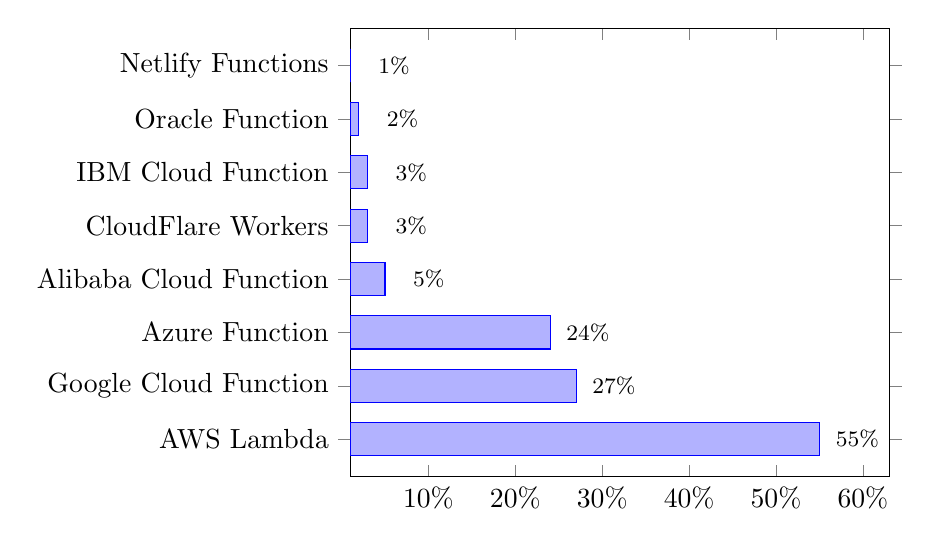
\begin{tikzpicture}
        \begin{axis} [xbar = .05cm,
            bar width = 12pt,
            ytick = data,
            enlarge x limits = {value = .15, upper},
            symbolic y coords={AWS Lambda,Google Cloud Function,Azure Function,Alibaba Cloud Function,CloudFlare Workers,IBM Cloud Function,Oracle Function,Netlify Functions},
            xticklabel={\pgfmathprintnumber\tick\%},
        ]
        
        \addplot coordinates { 
            (55,AWS Lambda) 
            (27,Google Cloud Function) 
            (24,Azure Function)
            (5,Alibaba Cloud Function)
            (3,CloudFlare Workers)
            (3,IBM Cloud Function)
            (2,Oracle Function) 
            (1,Netlify Functions) 
        };
        \addplot[only marks, 
            nodes near coords,         
            every node near coord/.append style={xshift=25pt,yshift=0pt,anchor=east,font=\footnotesize},
            point meta=explicit symbolic,
            ] coordinates { 
            (55,AWS Lambda) [$55\%$]
            (27,Google Cloud Function) [$27\%$]
            (24,Azure Function) [$24\%$]
            (5,Alibaba Cloud Function) [$5\%$]
            (3,CloudFlare Workers) [$3\%$]
            (3,IBM Cloud Function) [$3\%$]
            (2,Oracle Function) [$2\%$]
            (1,Netlify Functions) [$1\%$]
        };     
        \end{axis}    
    \end{tikzpicture}
    \caption{Hosted serverless platform usage according to the CNCF survey \cite{CNCFServerlessSurvey2020}}
    \label{fig:hosted-serverless-platform-share-survey}
\end{figure}

\textbf{Amazon Web Services}, \textbf{Microsoft Azure} and \textbf{Google Cloud Platform} are distinguished as three providers with the biggest market share. Their services are classified into categories and described in more details, altogether with other vendors and companies providing their services in the serverless computing field.

\subsection{Amazon Web Services} \label{serverless-amazon-web-services}

As previously mentioned, Amazon was the company that pioneered the field of serverless computing. Over the years, it established the dominant market position, leading in the number of available services, characterized by high quality and undergoing constant innovation. AWS is an enterprise ready vendor, highly focused on the public cloud sector, providing most comprehensive network infrastructure and data centers.

Moreover, it comes up with rich collection of advanced tools. CloudFormation and AWS Cloud Development Kit enable developers to manage the infrastracture, utilising the Infrastracture as a Code (IaaC) paradigm. Furthermore, the AWS Serverless Application Model (SAM), that efficiently integrate with other AWS services, helps with developing, building and testing the created software. Besides, the essential services necessary to develop serverless applications (described below in more detail based on the official documentation \cite{AWSServerlessOffering}), AWS offers a wide range of services oriented towards artificial intelligence and machine learning that allow to train and deploy machine learning models, operates on documents, images or speech. Furthermore, AWS provides services capable of connecting and cooperating with various IoT devices, process multimedia or~help with managing business processes.

The AWS pricing model is considered as a major difficulty when it comes to accurately estimate the cost of running the service, but most frequently the variety and maturity of~services and tooling counterweight this downside.

\begin{enumerate}
   \item Compute
   \begin{itemize}
       \item AWS Lambda --- First FaaS offering available on the market, that allows to~execute the function without provisioning and managing the servers, automatically scaling the solution by running the code in a new instance in response to an event. AWS Lambda supports natively Node.js, Python, Java, C\#, Go and Ruby as execution environments, with a possibility to incorporate custom runtimes or container based environments, charging for the execution with the~millisecond granularity and ensuring consistent performance by enabling Provisioned Concurrency.
       \item AWS Fargate --- Serverless compute engine for containers, eliminating the need to manage the servers, choose instances and scale the cluster capacity, providing appropriate level of isolation and security.
       \item Lambda@Edge --- Enable to run the Lambda code at an AWS location closer to the users of the application, utilising the Amazon CloudFront as Content Delivery Network (CDN) to reduce the latency and improve the performance.
   \end{itemize}
   \item Data Store
   \begin{itemize}
       \item Amazon Simple Storage Service (S3) --- Storage service for objects, offering high data availability, scalability and performance. It provides the storage of~a~wide range of data for different use-cases, such as application data, backups, data lake, websites and other assets, ensuring their durability.
       \item Amazon DynamoDB --- Flexible, scalable and distributed key-value and document database, providing high performance and low-latency data access. Enables data caching, cross-region replication, fault-tolerance and data encryption, being a suitable solution for web and mobile applications.
       \item Amazon Aurora Serverless --- Autoscalable and fully managed configuration for~Amazon Aurora, which is a relational database compatible with MySQL and PostgreSQL, enabling higher performance and availability.
       \item Amazon RDS Proxy --- Fully managed and highly-available database proxy for~Amazon RDS, which is a service that provides hosting and scaling for other relational databases.
       \item ElastiCache --- In-memory data store, compatible with Redis and Memcached suitable for data intensive applications with high-throughput and low-latency data access.
   \end{itemize}
   \item Network and Content Delivery
   \begin{itemize}
       \item Amazon API Gateway --- Managed service, enabling to expose APIs and connect with other AWS services, providing real-time two-way communication via~REST or WebSocket API, billed accordingly to usage.
       \item AWS AppSync --- Another fully-managed and scalable service, capable of defining and handling the two-way communication using GraphQL API as well as the heavy-lifting and communicating with other AWS services to store and sync the data.
       \item Amazon CloudFront --- Fast, secure and programmable Content Delivery Network (CDN) hosting the data such as videos, images or applications, utilising the AWS edge network location to make the service globally scalable and accessible.
   \end{itemize}
   \item Application Integrations
   \begin{itemize}
       \item Amazon Simple Notification Service (SNS) --- fully managed publish-subscribe service enabling high-throughput, many-to-many messaging for communication between applications, microservices and application-to-person messaging.
       \item Amazon Simple Queue Service (SQS) --- message queueing service, allowing to~decouple components of the distributed systems, available in two types: standard (offering high-throughput and best effort ordering) and FIFO (designed for ordered messages delivered exactly once).
       \item Amazon EventBridge --- Scalable serverless event bus, enabling to integrate the~incoming messages from other SaaS offerings with the AWS infrastructure.
       \item AWS Step Functions --- Serverless function orchestrator, allowing to combine AWS Lambda functions into workflows based on business processes, visualising them and maintaining the application state between execution.
   \end{itemize}
   \item Analytics
   \begin{itemize}
       \item Amazon Kinesis --- Offers key capabilities of scalable and fully-managed event streaming service, processing and analyzing real-time video, audio and other data streams instantly, without necessity to collect the data.
       \item Amazon Athena --- Interactive and managed query service for Amazon S3 based on predefined schema, using standard SQL syntax to quickly analyze large-scale datasets
   \end{itemize}
   \item Security and Identity
   \begin{itemize}
       \item AWS Identity and Access Management (IAM) --- Required to manage users, groups and their access to AWS services and resources in a secure way, offered without additional cost.
       \item Amazon Cognito --- Provides authentication service and identity management that can be easily incorporated with various clients solutions on different platforms.
   \end{itemize}
   \item Development Tools
   \begin{itemize}
       \item Amazon CloudWatch --- Service providing application monitoring and observability, gathering logs, metrics and capturing events within the AWS resources. Enables to analyse the environment behaviour, troubleshoot issues and take automate actions based on numerous indicators.
       \item AWS X-Ray --- Tool that allows to analyze and debug distributed application behaviour across multiple services based on the request tracing, gathering the~execution metric to identify the application issues and performance bottlenecks, available for both development and production applications.
       \item AWS Amplify --- Suite of tools and services, helping developers build efficient and scalable applications for web and mobile platforms, providing possibilities to deploy the static sites, easily manage content or configure the application backends with authentication and data storage.
       \item AWS CodeStar, AWS CodePipeline, AWS CodeBuild, AWS CodeDeploy --- Set~of tools helping with the automation, continuous integration and deployment workflows for various applications.
   \end{itemize}
\end{enumerate}

\subsection{Microsoft Azure}

Microsoft is the second from the biggest three vendors that started offering its serverless computing services in 2017, by integrating them into the Microsoft Azure platform. It~also provides a vast number of services, giving a more flexible and configurable runtime engine, supporting more programming languages.

When investing in the serverless field, Microsoft decided to repurpose its existing proprietary software to be available and greatly integrated with the cloud. Microsoft Azure is eager to cooperate with various enterprise companies, especially using their software. Contrary to the AWS, Azure platform can more effectively interoperate with customers' data centers, enabling them to the gradual migration of on-premise software or operate in a hybrid cloud model. Azure platform also provides some powerful DevOps tooling and numerous services, integrating machine learning and artificial intelligence, exposing among the others cognitive services, chatbots and document, images and video analysis and recognition.

Nevertheless, customers frequently are not satisfied with the Microsoft Azure complex pricing model, due to complicated software licensing options that are hard to understand without outside support. Moreover, some of the services are considered less enterprise-ready, due to issues with quality of these services, technical support and lacking documentation or when managing and configuring some of them outside of the Azure platform.

The current serverless offering of Microsoft Azure is presented in more detail, according to the information available on the vendor website \cite{AzureServerlessOffering}.

\begin{enumerate}
   \item Compute
   \begin{itemize}
       \item Azure Functions --- FaaS offering from Microsoft, integrating with other services, executing in an event-driven manner and autoscaling based on demand. It provides tools for building and debugging functions locally, supporting implementations in .NET Platform (C\#, F\#), Java, Node.js (JavaScript and~Typescript), Python and PowerShell, billing the execution on a per second basis.
       \item Azure App Service --- Fully-managed platform for building, deploying and scaling web applicationsm written in .NET, Node.js, Java, Python and PHP, running in Windows or Linux containers, integrating with other services from Azure platform.
       \item Azure Kubernetes Service --- Highly-available and secure managed Kubernetes service, automatically provisioning serverless infrastructure based on the traffic, utilising open-source tools like Virtual Kubelet for provisioning nodes and~KEDA for event processing from various event sources.
   \end{itemize}
   \item Data Store
   \begin{itemize}
       \item Azure Blob Storage --- Scalable, secure and durable object storage, capable of~storing a large amount of unstructured data objects, suitable for cloud-native and mobile apps. It provides high availability and geo-replication, generating events pushed to other Azure services upon data changes.
       \item Azure Cosmos DB --- Fully-managed, globally distributed and multi-model NoSQL database service, guaranteeing low-latency data access and scalability, exposing APIs for SQL, MongoDB and Cassandra.
       \item Azure SQL Database --- Family of SQL cloud databases, providing optimized performance, data durability, backups capabilities and adapting to requirement changes.
       \item Azure Cache --- Managed in-memory data store, which can be utilised as~caching layer, providing high-throughput and low-latency operation time, scaling according to demand with geo-replication and Redis capabilities.
   \end{itemize}
   \item Network and Content Delivery
   \begin{itemize}
       \item API Management --- Service enabling API management across cloud and on-premise environments with unified management experience, focused on security and observability with fine-grained data exposition rules and integration with other services.
       \item Azure Content Delivery Network --- Secure and reliable Content Delivery Network (CDN), greatly integrated with other services from Azure platform, ensuring proper security level and analytics features.
   \end{itemize}
   \item Application Integrations
   \begin{itemize}
       \item Azure Event Grid --- Service handling the message routing from various event sources, working in a publish-subscribe model, ensuring scalability and high-reliability.
       \item Azure Event Hub --- Managed, scalable and geo-replicable real-time data streaming service, enabling to build dynamic data pipelines, capable of seamless integration with other Azure services.
       \item Azure Service Bus --- Reliable and scalable messaging services for a cloud, enabling to build communication between decoupled application components and~on-premise systems, providing various messaging models and offline delivery.
       \item Logic Apps --- Service enabling developers to build various workflows within containerized environments, integrating external services and enterprise SaaS offerings along with the Azure platform components.
       \item Azure Durable Functions --- An extension for Azure Functions, enabling them to execute stateful computation in a serverless environment by utilising the~Orchestrator that defines the state flow between subsequent functions.
   \end{itemize}
   \item Analytics
   \begin{itemize}
       \item Azure Stream Analytics --- Serverless real-time analytics, enabling to build streaming pipelines with similar SQL-like syntax, integrating with other platform services including artificial intelligence for more sophisticated use-cases.
   \end{itemize}
   \item Security and Identity
   \begin{itemize}
       \item Azure Active Directory --- Service enabling identity management, authentication and authorization capabilities for end users. Enhancing it with single sign-on to multiple SaaS applications, multi-factor authentication functionalities and integration with external identity providers.
   \end{itemize}
   \item Development Tools
   \begin{itemize}
       \item Azure Monitor --- Fully managed and scalable monitoring offering, integrated with numerous Azure services, providing operational telemetry to analyze the cloud and on-premise services behaviour and performance, allowing to query and visualize the data and trigger alarms based on thresholds or patterns detected by~artificial intelligence to proactively notify about anomalies or issues
       \item Azure DevOps --- Cloud hosted service, providing a fully-fledged set of operational tools such as code repository and task management capabilities, enabling configuration of continuous integration and continuous delivery pipelines along with building artifacts and deploying software to multiple platform or on-premise services.
   \end{itemize}
\end{enumerate}

\subsection{Google Cloud Platform}

Google introduced its serverless products from their cloud offering in 2018 into general availability, after a long period in beta. It is noticeable that the Google Cloud Platform offering is not as rich and varied, and the services are not as mature and configurable, as~those offered in the AWS or Azure catalog.

The vendor is looking to cooperate closely with companies trying to scale quickly and startups, rather than large enterprises. Besides the serverless platform, the provider is~highly focused on containerization and microservice architecture, with the leading in~the Kubernetes services along with strong open-source commitments and DevOps-friendly approach. Google Cloud Platform is a leader in fields of artificial intelligence, machine learning and big data, offering numerous services and capabilities based on the open-source frameworks and libraries maintained by Google.

The provider gives a better impression to its customers in terms of the ease of setup and user-friendliness of the platform. The pricing model is aimed to be more customer friendly, offering exceptionally flexible contracts, appealing to customers interested in using the cloud.

Google Cloud Platform services, based on the available offer \cite{GCPServerlessOffering}, are presented below:

\begin{enumerate}
   \item Compute
   \begin{itemize}
       \item Cloud Function --- FaaS platform from Google, enabling to run the code without server management, scalable with the size of workload. Currently it supports Node.js, Python, Go, Java, .Net and Ruby runtimes. It is priced based on~number of invocation and execution duration with granularity to 100ms.
       \item Cloud Run --- Scalable and fully-managed container-based execution environment built on top of the Knative open-source project, triggered based on various platform events, automatically replicated across multiple regions and billed according to actual usage.
       \item App Engine --- Hosting platform for mostly web applications written in Node.js, Java, Ruby, C\#, Go, Python, or PHP, responsible for managing the infrastructure and scaling the solution
   \end{itemize}
   \item Data Store
   \begin{itemize}
       \item Cloud Storage --- Object storage ensuring security, durability, data access with low latency and geo-redundancy, enabling to store data across different storage classes characterised with different parameters and cost.
       \item Cloud SQL --- Managed and cloud-based relational database service for MySQL, PostgreSQL and SQL Server, ensuring reliability, automate database provisioning and storage management.
       \item Cloud Spanner --- Database with relational semantics and strong consistency with unlimited scaling, delivering high-performance transactions across regions, automatically handling scaling and sharding
       \item Firestore --- Serverless NoSQL document database, scaling with the demand with no maintenance overhead, with built-in live synchronization, ACID transactions and offline support. Designed to be used with mobile, web and IoT applications with direct connection to the clients, integrating with other Google Cloud Platform services.
       \item Cloud BigTable --- Fully-managed and scalable NoSQL database service, designed for machine learning and big data services, seamlessly scaling to~the~storage needs, capable of processing high-throughput data with low latency
       \item Memorystore --- Low latency, scalable and secure in-memory service, compatible with Redis and Memcached, enabling high-availability, automatic failover, patching and monitoring.
   \end{itemize}
   \item Network and Content Delivery
   \begin{itemize}
       \item Cloud Endpoints --- Development, deployment and management tool for APIs, providing logging, monitoring, access control and integrations with third party services as identity providers.
       \item Cloud CDN --- Globally distributed and reliable Content Delivery Network (CDN) for images, videos, webpages integrating with other services and supporting hybrid and multi-cloud architectures.
   \end{itemize}
   \item Application Integrations
   \begin{itemize}
       \item Cloud Pub/Sub --- Event-driven messaging system and analytics stream, auto-scalable, with no provisioning and cross-zone message replication, enabling in-order messaging with push and pull models
       \item Cloud Tasks --- Fully managed service that allows to handle and distribute vast number of distributed tasks asynchronously, building more decoupled applications in microservice architecture that can be scaled independently
       \item Cloud Scheduler --- Managed cron job service suitable for batch and big data jobs as well as cloud infrastructure operations, automating tasks management and handling retries in case of failures.
       \item Workflows --- Workflow orchestration service, integrated with multiple Google Cloud Platform components, focusing on modeling workflow logic, executing it~in~a~reliable way, passing the execution state between particular steps.
   \end{itemize}
   \item Analytics
   \begin{itemize}
       \item BigQuery --- Serverless data warehouse based on real-time data stream with autoscaling and managed infrastructure, enabling multi-cloud capabilities, integrated with many tools and services of Google Cloud Platform in the fields of machine learning, artificial and business intelligence.
   \end{itemize}
   \item Security and Identity
   \begin{itemize}
       \item Identity and Access Management (IAM) --- Service provides management capabilities for fine-grained access control for Google Cloud Platform resources along with monitoring and auditing them.
       \item Cloud Identity --- Service providing unified Identity and Access Management for~applications and endpoints, enforce strong security and access control, enabling access to thousands of applications via single sign-on
   \end{itemize}
   \item Development Tools
   \begin{itemize}
       \item Cloud Build --- Serves as a serverless service for building, testing and deploying artifacts and applications, utilising integration and continuous delivery pipelines
       \item Cloud Logging --- Real-time log management and analysis services, capable of~extracting data from logs and analyzing them in real-time.
       \item Cloud Monitoring --- Service for collecting metrics from various sources, visualising them. It monitors applications and services behaviour, and integrate with other third party solutions to provide better visibility and observability of~the~system.
       \item Cloud Trace, Cloud Debugger, Cloud Profiler --- Set of tools helping developers with tracing events in the distributed system and collecting numerous metrics, debugging the production application to get more insight into their behavior and profiling the application performance and resource utilisation.
   \end{itemize}
\end{enumerate}

In addition to the Google Cloud Platform services, Firebase \cite{Firebase} is another and~independent service, backed by Google and based on their cloud platform, providing BaaS components that can be directly integrated with web and mobile clients. All of the services are auto-scalable and with the infrastructure managed on the provider side. The~core~feature is a real-time document database utilising Firestore underneath, integrating with Cloud Functions, Cloud Storage and providing authentication capabilities. Moreover, the~offering includes other components that allow developers to monitor the performance and stability of applications as well as analyse the customers behaviour using A/B testing, boosting their engagement by in-app and cloud messaging.

\subsection{Other cloud providers and services}

\subsubsection{IBM}
IBM Cloud focuses on helping enterprises migrate to the cloud, extend their capabilities and transform their workloads to be more agile utilising cloud infrastructure. Over~the~years the company invested in industry-focused cloud services and hybrid cloud market, supporting diverse workloads including SAP, Oracle ERP and newer technologies including machine learning capabilities. Company promotes the open-source initiatives to~produce the~results, along with portable components that can be used among multiple cloud providers \cite{Gartner}.

In terms of serverless components, IBM Cloud Functions is based on open-sourced Apache OpenWhisk platform, which manages the infrastructure and scaling using Docker containers and can be deployed independently on top of popular container frameworks like Kubernetes, Mesos or OpenShift. The platform supports a programming model in which functions (called Actions) are dynamically provisioned in response to associated events (called Trigger) coming from numerous external sources or HTTP requests. Currently, OpenWhisk supports a large number of environments, such as Node.js, Go, Java, Scala, PHP, Python, Ruby, Swift or any executable running inside the Docker container \cite{ApacheOpenWhisk}.

\subsubsection{Alibaba Cloud}

Alibaba Cloud is a cloud provider that have a strong ties with Chinese public sector as~well as cooperates with numerous companies operating in the China and Southeast Asia region. The cloud vendor supports its clients with cloud migration and helps traditional enterprises to build their presence in the digital platforms. Most of its clients reported satisfaction with the platform solutions, but the limitations can be noticed in a modest international offerings compared to the services available in China region. Moreover, the~discrepancies in documentation and functionalities availability \cite{Gartner} occur.

The Function Compute is a serverless FaaS offering with a pay-as-you-go model, managed and scaled by~the cloud provider in response to events incoming from various data sources. It supports mainly Node.js, Python, Java, PHP, C\# and custom runtimes in~containers. The cloud platform provides two function instances --- the flexible functions, and~instances with the higher specifications for better performance. Additionally, vendor offers reserved instances that are always on, reducing the ''cold start'' \cite{AlibabaFunctionCompute}.

\subsubsection{Cloudflare}

Cloudflare is a company providing services in areas of web infrastructure and website security, such as Content Delivery Network, domain name servers and internet security services, serving as reverse proxy for websites. It also provides numerous analytics that gives insight into transfer speed, incoming traffic from unique users and their geographic location.

From serverless offerings, Cloudflare Workers are a FaaS platform based on the edge computing, providing high-performance. The solution is also managed, auto-scalable and~billed in a pay-per-use model, similar to other serverless offerings, but the difference is~in~the Cloudflare's edge network, that routes the request to the closest location where the function is executed, limiting the latency and providing high availability. Currently, the platform supports Node.js, Rust, C, and C++ as~an~execution runtimes \cite{CloudflareWorkers}.

\subsubsection{Oracle}

Oracle Cloud is expanding its worldwide presence and their cloud services into numerous regions, developing hyperscale cloud architectures that are competitive with other, more-established cloud providers. The vendor tends to cooperate more closely with enterprises, using its business applications and enable to incorporate and integrate them within the~cloud~platform. All of the cloud offerings are available in multiple regions with the same capabilities \cite{Gartner}.

Oracle Cloud Functions are offered in pay-as-you-go model, managed and scaled by~the provider and they are based on the open-source Fn Project and CloudEvents, which is~an~open-source specification for describing event data. It supports Go, Java, Node.js, Python, Ruby and C\# programming languages and custom runtimes using Docker to~execute the functions. The platform is vendor-agnostic and can be also executed in private and hybrid cloud \cite{FnProject}.

\subsubsection{Netlify}

Netlify is offering hosting and serverless backend services for static websites and web applications. The deployment process is easy and convenient for developers, which can connect Git repositories with the platform, enabling automatic continuous deployment triggered with every code change. Netlify extended its portfolio with other services such as serverless form submission, user identity management, analytics and also their own headless content management system, which can be utilised by dynamic web applications.

Currently, the offer also includes serverless functions powered by AWS Lambda, that can be automatically provisioned when the platform detects the configuration in the linked repository. The Netlify Functions can be triggered based on HTTP request to the defined API endpoint or form submission, as well as enabled to run asynchronous processing in~Background Functions with longer execution time. Altogether with the whole platform, it allows developers to quickly and easily setup the production environment for the web application or static website without any operational knowledge \cite{NetlifyFunction}.

\subsection{Open-source alternatives}

The benefits of serverless architecture, such as cost reduction and eliminating the need of~infrastructure management, became an appealing argument to use the technology. Nevertheless, some companies invested heavily in their hardware infrastructure, are afraid of~the~vendor lock-in or computation restriction of the public cloud platforms. Open-source frameworks are promising to overcome these limitations and manage the serverless components on self-hosted environment or hybrid clouds.

According to the aforementioned survey conducted by CNCF \cite{CNCFServerlessSurvey2020}, the most popular solution in the category of installable software for serverless function execution is~newly added Knative (claimed to be used by 27\% of respondents), while OpenFaaS maintains its~popularity (used by 10\% of interviewee) with Kubeless (mentioned by 5\% of~respondents).

All of the projects are based on the Kubernetes as a portable and extensible platform, enabling declarative configuration and management for containerized environments. Serverless frameworks rely on it to orchestrate and manage the serverless functions inside containers, schedule their executions, provide service discovery and replication. Each of~the open-sourced serverless frameworks approach the container orchestration is slightly different. For example, OpenFaas provides its own API Gateway, providing access to~the function, collecting metrics and scaling the solution, while others like Knative, utilise third party Ingress Controller for Kubernetes and manage the scaling by Queue-Proxy Container, passing the events to functions inside the pod. Several articles consider the~viability and quality of services for the open-source serverless platforms \cite{OpenSourceServelessPerformance}, considering also interesting possibilities of utilising serverless in edge computing \cite{OpenSourceServelessEdge}.

Nevertheless, utilising open-source platforms raises questions about maturity of these frameworks and introduces another set of challenges, which need to be researched and~addressed. Based on the previously mentioned papers some of the self-hosted serverless platforms show issues with scaling, lack of predictability and guaranteeing good quality of~service. Each of the frameworks provides default fault tolerance for container runtime, limited to retrying the execution which sometimes may be not suitable. All~of~the public cloud providers mendtioned above tend to supply various tools and services that support developers with log aggregation, monitoring, alerting and distributed tracing across the~serverless components, which requires manual integration in the open-source alternatives. Public cloud vendors offer not only the FaaS platforms, but also provide a~large variety of~BaaS components that can be integrated with serverless functions to build fully-fledged applications and services. This is in contrary to the open-sourced alternatives, which focus solely on the FaaS platforms. While the other components could be~also self-hosted, integration with them as well as scaling requires manual management on~the~customer side, increasing the amount of work that needs to be done to maintain the services quality and going against the idea of serverless.

\section{Example use cases} \label{chapter:serverless-example-use-cases}

\subsection{Application backend} \label{chapter:serverless-example-application-backend}

Serverless technologies are an appropriate solution for building scalable application backends for all kinds of web, mobile and desktop applications. They are favorable for this use-case, because the infrastructure management can be effectively automated, ensuring dynamic scaling to meet uneven demand, with proportional and predictable billing. Despite the fact that serverless technologies are a relatively new approach to building services, some of the companies have already used it to power large applications.

To build the application backend, serverless functions are used to transform the data representing the application logic, together with other third party services capable of persisting data or exposing some desired functionalities. The API Gateway provides uniform access to various serverless functions using REST API, preserving mapping between requests and respective serverless functions, enabling integrations with other services, for~example responsible for authentication and authorisation. Sending a request to the API can lead to execution of one or more serverless functions, containing custom business logic and~communicating respectively with other services. It is also possible that the frontend application can communicate directly with external components, bypassing the API Gateway. Nevertheless, it is essential to handle the communication in a secure manner using the~delegation tokens \cite{ServerlessArchitectureOnAWS}.

\begin{figure}[h]
    \centering
    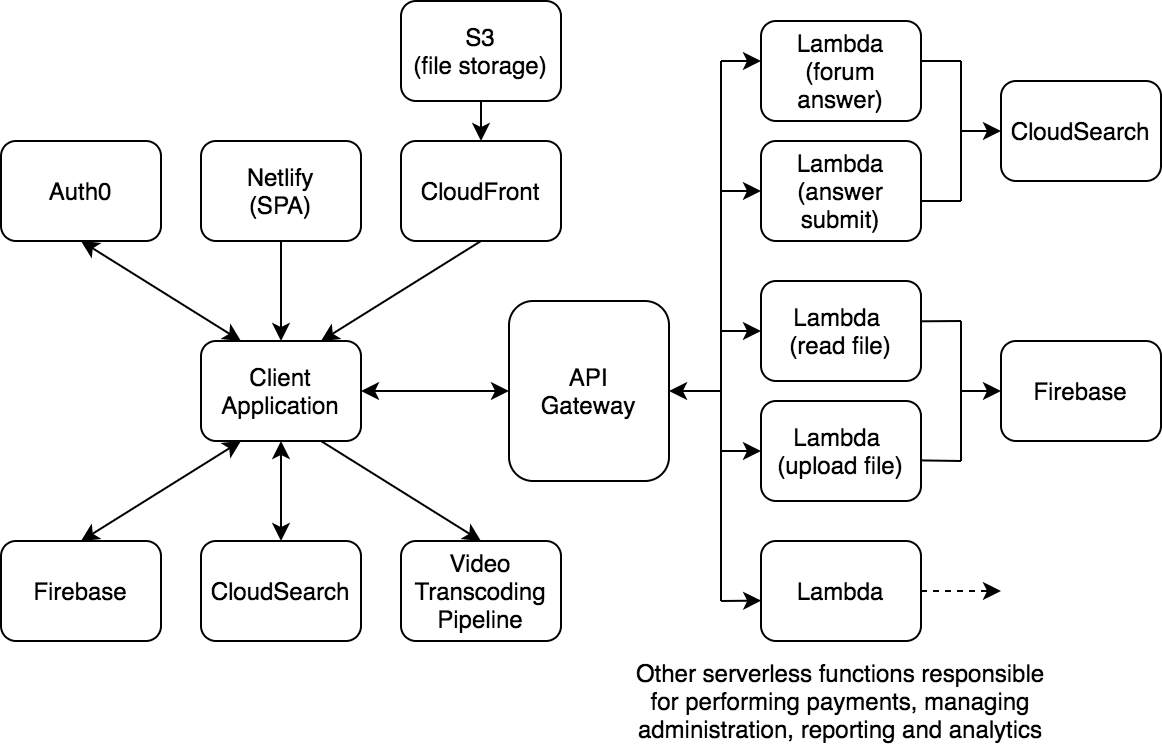
\includegraphics[width=0.8\textwidth]{assets/02-serverless/CloudGuruArchitecture.png}
    \caption{CloudGuru platform architecture}
    \label{fig:cloudguru-architecture-diagram}
\end{figure}

CloudGuru, which is an online educational platform dedicated to people interested in~learning numerous cloud related topics, is a good example of such an use-case. Core~features of the platform include streaming large selection of video courses, interactive quizzes and practice exams, real-time discussion forum and integrations with third party services, enabling users to buy access to the courses.

The architecture of the e-learning platform utilises services of several cloud providers. Frontend of the web application built as a Single Page Application is hosted on Netlify, which acts as a Content Delivery Network (CDN) for the web client. Auth0 service is~responsible for authentication functionalities and provides delegation tokens for client application, communicating directly and securely with other services. Firebase is used as~a~primary database, which is capable of updating clients in real-time using WebSockets to push the data to the client applications. Questions and answers submitted by users to the forum are persisted in the Firebase, with the data being sent further to the AWS CloudSearch, which is indexing it for searching purpose and enabling users to later find information easier. Instructors can upload video directly to S3 bucket, that triggers the~video transcoding pipeline. Users can watch the videos served via CloudFront acting as~a~CDN, if they call the Lambda function beforehand, which gives them the permission to~access the video assets for a limited period of time.

\subsection{Event-driven data processing} \label{chapter:serverless-example-event-drive-processing}

Serverless has also found application in numerous media conversion and transcoding as~well as various data processing tasks. When the new file is inserted to the bucket responsible for data storage, it can trigger a serverless function passing the necessary data and file as~an~event to perform the processing. Such an event-driven approach is suitable for~building pipelines for data-processing tasks, billed only for the function execution time and other BaaS components usage to transfer, transform or extract some information \cite{ServerlessArchitectureOnAWS}.

\begin{figure}[h]
    \centering
    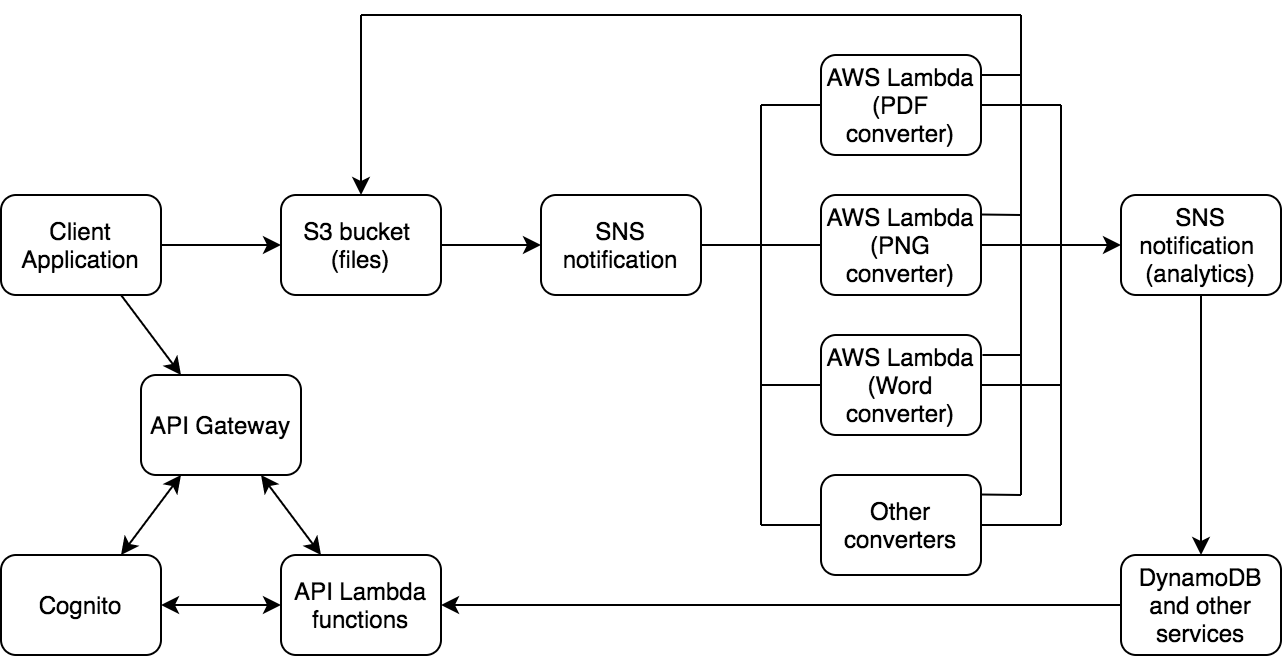
\includegraphics[width=0.8\textwidth]{assets/02-serverless/MindMupArchitecture.png}
    \caption{MindMup platform architecture for file export}
    \label{fig:mindmup-architecture-diagram}
\end{figure}

An example of such serverless utilisation is MindMup, which is a popular web application serving a role of a mind mapping tool, which was initially developed by just 2 developers. The event-driven data processing is utilised when a user wants to export prepared diagram to some read-only format such as PDF, Word document, presentation or text file. The web application works as interactive user interface. Upon user requests to export the~diagram, it calls the Lambda placed behind the API Gateway to generate the presigned URL, which can be used for a short period of time to insert the file directly from the client application to the S3 bucket. It sends an event to the Amazon Simple Notification Service (SNS) triggering the appropriate function responsible for export to~a~particular file format. Each of the exporters have different requirements, for~example CPU and memory usage for PDF exporter is much higher than for others, while Microsoft Office exporters require usage of libraries written in Java. Moreover, some of~the extensions such as Markdown are not as frequently selected by users. When the processing is~complete, the output of~the process is inserted to the S3 bucket, where the users can access it. Additionally, the event is sent to SNS which triggers other services such as DynamoDB, that are listening to that topic to save some information for analytics purpose.

The company admits that initially, the service responsible for exporting was running on the Heroku platform in the containerised environment, but after migration to the AWS Lambda, they have noticed significant cost reduction even with the growth of the platform usage by the clients \cite{ServerlessApplicationsWithNodejs}.

\subsection{Real-time stream processing}

Serverless architecture also found application in the data ingestion tasks from numerous data sources, such as logs, system events, transactions or social media feeds that need to~be~analyzed, aggregated and stored. Utilising BaaS components capable of event stream aggregation over time with the serverless function which can be configured to run when the specific number of records (forming a batch of records) is available. Such a messaging pattern is popular in distributed systems, where it allows to decouple the services and~provides reliability by storing the messages in the queue, when the consuming service cannot process more data at the moment, additionally providing retry mechanism in case of failures \cite{ServerlessArchitectureOnAWS}.

\begin{figure}[h]
    \centering
    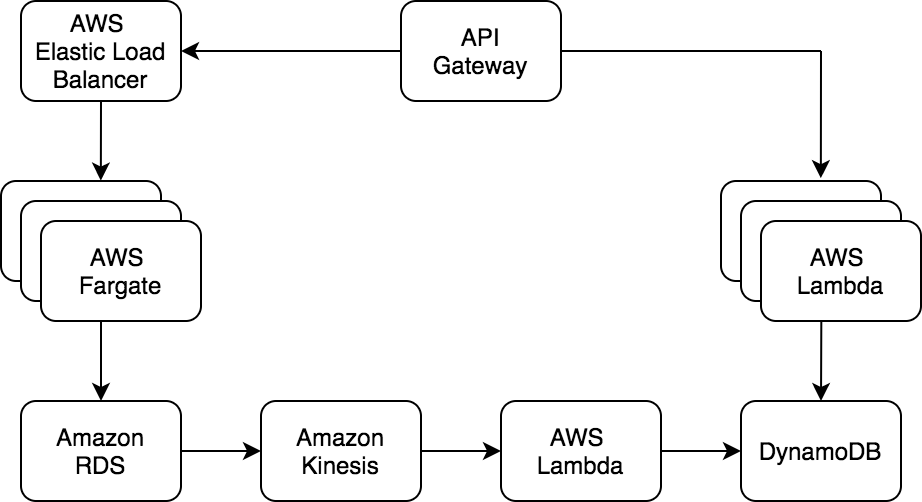
\includegraphics[width=0.7\textwidth]{assets/02-serverless/TemenosArchitecture.png}
    \caption{Temenos platform architecture}
    \label{fig:temenos-architecture-diagram}
\end{figure}

Temenos, as one of the largest banking software providers, is using such a pattern along with other serverless technologies in their T24 Transact banking system to achieve a highly elastic solution with low maintenance cost. It supports a large number of interactions and transactions between banking customers worldwide. Due to leveraging the platform and managed services, it reports that even the unpredictable workloads due to peaks in the market are handled efficiently. All the requests coming to the systems are getting through the AWS API Gateway. It passes them to the AWS Elastic Load Balancer (ELB), responsible for routing the requests to proper container instance running on AWS Fargate. The application running inside the container, performs the business actions based on the request and persists the result in Amazon Relational Database Service (Amazon RDS) that is an Online Transactional Processing Database (OLTP) designed to process the transactions effectively. Later, the stream of data and more complex business events is~pushed from Amazon RDS to Amazon Kinesis, which aggregates the data and triggers the AWS Lambda responsible for processing it, to build a query-optimized data model which is stored in DynamoDB. When the banking system users want to read the data, they perform a request that goes from API Gateway to AWS Lambda, that queries the~read-optimized data model from DynamoDB \cite{ThisIsMyAchitectureTemenos}.

\subsection{IoT applications}

With the growth of smart homes popularity, IoT devices along with other machines that are meant to help people, started incorporating more sophisticated technologies to support people on a daily basis. iRobot is a leading company in terms of designing and building smart robots, helping people around their household, with the Roomba robotic vacuums as their most popular product. Besides robotics, the company provides iRobot HOME application which enables customers to interact with their smart home devices.

\begin{figure}[h]
    \centering
    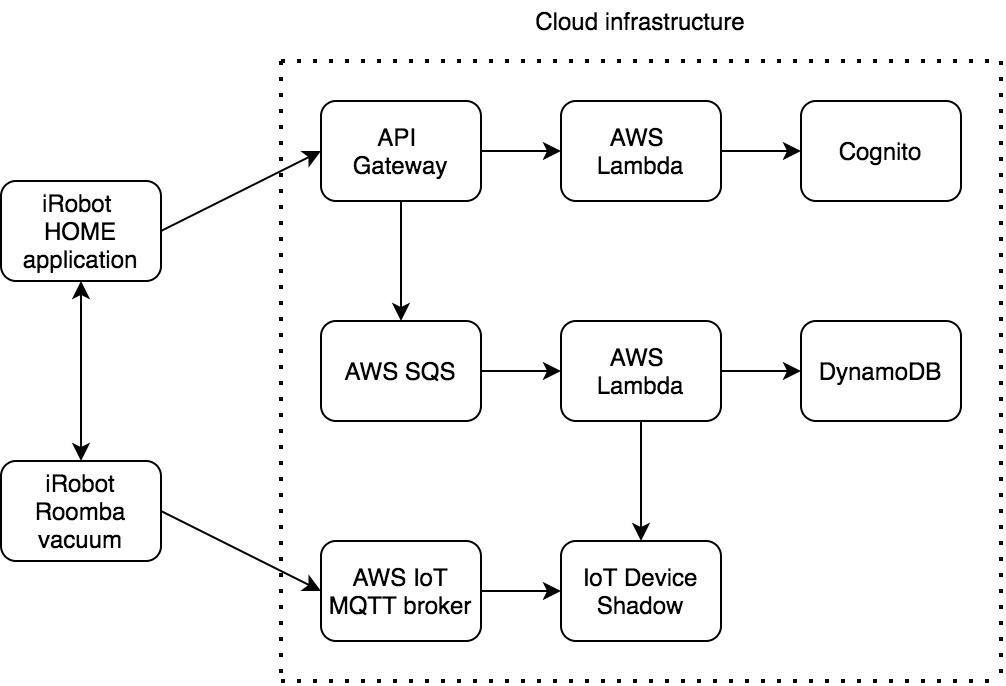
\includegraphics[width=0.7\textwidth]{assets/02-serverless/iRobotArchitecture.png}
    \caption{iRobot solution architecture for smart robots}
    \label{fig:irobot-architecture-diagram}
\end{figure}

AWS IoT is an entry point for the Roomba vacuums to connect them with the cloud. For the communication purposes MQTT is used, which is a lightweight publish-subscribe protocol for IoT devices. The AWS IoT Shadow Device provides asynchronous communication mechanism, enabling the robot to work properly without the constant communications with the cloud. When the smart vacuum finishes cleaning job, its data is synchronized with the cloud, which allows users to update the cleaning schedule, accordingly to changes made in the iRobot HOME application. Along with the AWS IoT, developers can define additional IoT Rules that configure the device to connect with other services in the cloud, for example to update the device status along with its parameters or informing users that the vacuum tank is full. Moreover, it gathers additional information about usage and~home~mapping to better plan device's tasks and manage the battery power \cite{ServerlessIoTatiRobot}.

Developers and designers of the robotics solutions observed many benefits related to the utilisation of cloud vendor services and the serverless paradigm, mentioning the scalability of the solution without the need to manage infrastructure and significant cost reduction, while preserving the proper level of security and data privacy \cite{AWSIRobotIoT}.
\chapter{Web applications}

% aplikacje webowe - czym się charakteryzują?
% jakie założenia trzeba spełnić? jakie wymagania stawiane są przed deweloperami?
% ---
% What are the core ideas of web applications?
% what are the requiremenst from the system / components perspective?
% What architectures are commonly used?

\section{Origins}

The idea of web applications has been changing over the years alongside the increased interest in using them. Currently, web applications can take a variety of forms, which lead to the emergence of various architectures and solutions suitable to develop efficient and user-friendly software working in the browsers. Niels Abildgaard \cite{PerspectivesOnArchitectureEvolution} analyzed in a great detail how the perspective of web application developed over the years, discussing the variety of web application architectures and some of the common patterns and architectures used in their development nowadays.

The initial idea of the World Wide Web was to exchange informations easily with a broader audience. To achieve that the client-server architecture was used allowing clients to request servers for desired information. The client could make a request to the server using HTTP protocol and receive some static content (in form of HTML file or other static assets) or dynamically generated content (returned as a result of program execution triggered by the server). The term web applications is more suitable for the latter one, which represents a more interactive type of website, including some business logic and returning the dynamic response based on that.

The growth of server-side logic and it's complexity influenced the idea of splitting it into numerous Web Services responsible for particular part of application logic and communicating with other clients or servers. Service-Oriented architecture encouraged developers to split larger applications and enable them to cooperate using standardized communication protocols. Introduction of Representational State Transfer (REST) refined the client-server communication to be stateless, enabling cacheability and uniform communication using HTTP protocol.

Another idea which enabled developers to deal with the complexity of web application was to differentiate between specific layers in web application architectures. Early web applications distinguished presentation layers displayed to the users, which communicated with the business logic layer utilising data layer for persisting data. Other modern frameworks utilised Model-View-Controller (MVC) approach, in which the visual part was represented by the View, Controller based on the request was responsible to interact with the Model containing necessary data and business logic.

Next factor which led to enhancing the interactivity in the browser was the emergence of Ajax (Asynchronous Javascript and XML), allowing to load data dynamically and asynchronously without reloading the whole page. Growth of Javascript popularity enabled developers to build more interactive and dynamic applications detached from the initial markup, called Single-Page Applications. Additionally, more and more business logic started to be implemented on the client side of web applications, which became thicker clients providing better user experience similar to desktop applications.

Alongside the technology evolution, the requirements that the web applications need to fulfill are also developing, most often pushing them to the limits, providing better user experience while working on more demanding computation and processing larger amounts of the data than before. To meet such requirements some modern architectures and approaches emerged allowing to achieve desired capabilities, most frequently resulting with some tradeoffs.

---

TODO:rb - sum up patterns and architectures described later in the chapter

% server

% - scalable and efficiently handle large number of users making many frequent data retrieval and updates
% - growth of complexity of business logic - various patterns to handle that - smarter models than CRUD -> DDD, thinking about events
% - SOA -> to fix tangled dependencies, microservices that can be independently developed, managed and scaled

% client

% - web browsers capable of executing dynamic client-side behaviour
% - thick, highly rich and interactive clients with desktop like experience
% - increase in javascript engines in modern web browsers has lead to the development of many new web application architectures
% - large initial load of SPA, static site generators/JAMstack for context that rarery changes
% - PWA as web apps behaving as native mobile of web application, caching, working offline, accessing more native features of mobile devices
% - techniques to have high interactivity, but on the other side to optimise load time, performance
% - moving beyond req/res pattern, to proivde more direct communication - websockets

% database

% - users consume and produce lot of content, manipulate large amount of persisted data
% - emergence of NoSQL solutions - more scalable and efficient especially when working on large amount of data concurrently
% - NoSQL databases tend to have more relatex relations to the principles (ACID) in favour of speed and simple replication abilities


\section{Defining web application}

Taking into account the various types of web applications and numerous purposes they may serve, it can be difficult to clearly present the core ideas of web application. Researchers tried to define the term web application to describe the wide range of web applications. One of the definitions can be found in ''Web Application Architecture'' published by Leon Shklar and Richard Rosen \cite{WebAppArchitecture}.

\begin{quotation}
A Web application is a client-server application that (generally) uses the Web browser as its client. Browsers send requests to servers, and the servers generate responses and return them to the browsers. They differ from older client-server applications because they make use of a common client program, namely the Web browser
\end{quotation}

Nevertheless, the perspective of web application has been changing over the years as well as along with requirements they face. Web servers providing mostly static content changed into more complicated applications, that consist of multiple layers where each of them is responsible for a selected fragment of processing client request. For more complicated use-cases it was not enough and the server application took the form of a distributed system, that consist of multiple services communicating with each other to process the application logic. Alongside with the development of server application, the database management systems have been evolving, presenting new paradigms to meet the requirements of the web applications using them. Lastly, the presentation layer of web applications also changed rapidly, resulting in dynamic and interactive client-side applications including parts of business logic.

Niels Abildgaard also noticed the progress of technologies and architectures used in web application development and proposed another definition of web application based on his research \cite{PerspectivesOnArchitectureEvolution}.

\begin{quotation}
A web application is a client-server application with any number of clients and servers, in which client-server communication happens via HTTP, in which both client and server may be execution environments, and in which the server may be any arbitrarily complex system in itself.
\end{quotation}

Taking into account both definitions, we can refer to web applications used currently as mainly two communicating with each other parts - client (preferably used by web browser) and server, which can be any complex system by themselves.

\section{Requirements}

Having described the development of web applications over the years it is relevant to consider what were the requirements placed on the web application that lead to such a development process. Currently, web applications can operate in numerous areas and based on the business needs, target various customer groups and other non-functional requirements - the desired capabilities they need to fulfill may differ. For example, a small e-commerce shop serving a handful of customers a day within one country will have different requirements than a large social network in which millions of people participate worldwide, on a daily basis. Nevertheless, several generic requirements applicable to the majority of web applications can be distinguished, but the importance of them and to which extent they should be incorporated may differ depending on the application use-case and its scale.

\subsection*{Performance and Scalability}

The performance of web applications can be considered from two separate perspectives - user and system point of view \cite{DesignDataIntensiveApplications}. In the first case we can think of the user's interactions with the web application and the time that it needs to respond to requests made by the user. To define how the application should behave terms such as service level objectives (SLOs) and service level agreements (SLAs) can be introduced to characterise the expected performance and availability of web application (for example if the service median response is served within 200ms and for the 99th percentile is under 1s). Nonetheless, for most of the time the user is not using the application alone. The interactions of numerous users need to be taken into account by various components of the underlying application that need to handle them efficiently. When the load increases (in terms of the traffic, data volume or complexity of actions) the system should scale accordingly to reasonably handle the traffic without performance degradation. 

Scaling can be referred to as the ability to cope with increased load which can take various forms, for example number of requests per second, read to write ratio for database or number of simultaneously active users. To achieve that two different approaches can be used: scaling vertically (using more powerful machines) and scaling horizontally (distributing the load across multiple smaller machines). Some of the systems can automatically scale by allocating new computing resources based on the metrics related with traffic or performance, which is a desirable feature especially when the load is unpredictable. By building applications servers in a stateless manner, the horizontal scaling can be easily used to meet the demand. Unfortunately, stateful components can be harder to scale. Some storage components are designed and implemented to handle scaling gracefully, for other components techniques such as data fragmentation or replication have been introduced to meet the desired performance requirements.

\subsection*{Reliability}

Reliability refers to the fact that the system should continue to work correctly (perform correct processing as user expected at desired level of performance) even when the faults occur \cite{DesignDataIntensiveApplications}. The designed system should be resilient and fault-tolerant, preventing the web application from stopping providing the service to users. The aforementioned service level agreement (SLAs) metric can also refer to the uptime of the services, stating for example that not less than 99.9\% of availability time within a month is acceptable.

The origin of fault may be different, but some of the major factors can be hardware faults, software errors and bugs and human errors introduced while developing and managing the application. To prevent them various techniques can be introduced. Hardware faults in form of hard disk crash, power grid blackout or network cables that are not plugged in properly can be masked by introducing redundant components that are utilised until the broken component is replaced or fixed. Software errors in the form of introduced bugs or other human errors related with configuring services can result in unexpected and undesired behaviour of application or even other components of the system. That area of errors is harder to mitigate, but proper manual and automation testing can prevent from introducing errors, while monitoring and analysing service behaviour in production will raise an alert if some deviation is noticed.

The reliability is expected not only from larger web applications, but also from smaller one. Downtime and software bugs in the web application can contribute to loss in revenue and damage the reputation.

\subsection*{Security and Compliance}

These days web applications became one of the most popular platforms for exchanging information ranging their utilisation from numerous social media platforms to more critical areas such as bank accounting or accessing sensitive and confidential information stored on some servers in a digital form. The security breach of some web applications could result in compromising large amounts of sensitive data, leading to severe legal and economical consequences. Along with the growth of web application ecosystems the attack surface enlarges and the risk of introducing some security vulnerabilities is increasing.

It is substantial to ensure a proper level of security based on guidelines and frameworks defined by organisations and authorities working in the field of security, hardening the web application and mitigating the possible attacks to ensure compliance with security standards. Web application design should ensure that users identity and sensitive information are properly secured, giving access to resources only when the user identity is verified along with expecting adequate permissions \cite{ASurveyonWebApplicationSecurity}.

\subsection*{User Experience}

Modern web application clients are more frequently becoming more complex, interactive and feature-rich applications including larger parts of business logic. The success of products based on web applications is more frequently connected with the fact how the user perceives it and it is becoming more important to make sure that application interface is aesthetic, while the overall user experience of the application is intuitive. Nevertheless, the user interface is not the only factor impacting how the user perceives the application, the efficiency and performance also plays a significant role, which is correlated with the whole system design.

The idea of user experience (UX) is quite a broad term on the verge of cognitive science and human-computer interactions. It is considering not only the interface design, but also the system usability, ergonomics and performance, inspecting how the users feels when interacting with the system. Enhancing user experience is one of the main goals of user-centered design, inspecting the perception of the value of the system, how easy and efficiently users can perform various tasks and looking into processes within the system, if they are intuitive and pleasant for users. Many companies are using different analytic tools nowadays  to understand how users utilise the products.

The diversity of users and platforms also plays an important role. One of the consequences of that is the fact that many applications are suitable to use from mobile phones, because more and more people use smartphones on a daily basis. Also accessibility issues are gaining more awareness to make web applications suitable for people with some of disabilities \cite{WhatIsUserExperienceDesign}.

\subsection*{Maintainability}

Although maintainability may not be the obvious requirement for web application, it is an important factor for business executives, developers and people working in operations. Majority of the costs from a product development perspective is not the initial version of application, but it is related to the maintenance taking form of keeping the system operational, fixing bugs and resolving failures \cite{DesignDataIntensiveApplications}.

To maintain the software efficiently, the operational aspects such as monitoring, patching, deployment and maintenance of a stable environment should be easy and mostly automated to make sure the system is running smoothly. From an engineering perspective the system should be simple, by removing unnecessary complexity connected with tight coupled modules, tangled dependencies and inconsistency in terminology or architectural patterns. By reducing the complexity the maintainability of the application will be easier. It will also increase agility and make the evolution of the system easier, which will result in reducing time of introducing new features and reacting to architectural changes required to make the system operate efficiently.

\section{Modern web application architecture}

There are many potential perspectives considering the architecture of modern web applications when taking into account the areas they operate on and specified requirements that they need to fulfill. Below some of the used patterns and techniques used in modern web application architectures are discussed, allowing systems to meet the desired requirement and specification while working efficiently. It is divided into three sections taking into consideration the web application client which is the user interface that the user interacts with, which communicates with the server-side application tier responsible for performing the business logic using the underlying data layer to persist the application state. However, some of the discussed patterns goes beyond such classification, especially when they are referring to the communication between layers boundaries.

\subsection*{Server Application Tier}

\subsubsection*{Microservice architecture}

Microservices is one of the trends in modern web application development gaining more interest, especially when taking into consideration various benefits and success stories of the biggest companies using it to run their services in the web. To consider microservices it is useful to compare it with the monolithic architecture, which refers to building server-side applications as a single logical executable unit responsible for handling the HTTP requests, execute the domain logic, retrieve and update data in the database and send back the adequate response. Such architecture can be effectively applied when building simple applications, but when the system grows and evolves over time it is harder to preserve good modularisation and keep changes within the modules they should belong to, expanding unnecessary complexity into other parts of the system. Altogether with the system growth, it may require to be scaled accordingly to the load. It can be achieved by running multiple instances of the server application behind load balancer, but it requires to scale the whole application, rather than particular components that require more resources. Another downside of the larger applications built as a monolith is the fact that every change requires rebuilding and deploying the whole application including the parts of the system, even not affected by changes.

Microservice architecture is described as a solution for these problems. We can refer to microservices as an approach to developing applications as a set of small services, that each of them run on its own and communicate via message passing using standard data formats and protocols via well-defined interfaces. Each of the services is built around specific business capabilities providing module boundaries within a domain it operates in - mitigating the problem of good modularisation. Moreover, each of the components can be deployed independently reflecting the notion of agile development and gearing towards continuous deployment. Scaling can be also applied in a more granular manner affecting only the services that require more resources to perform effectively under the load. \cite{FowlerMicroservices}

Separating larger systems into independent services can help with ensuring firm module boundaries within the domain of the system. It makes it easier to maintain the components overtime and introduce required changes independently from other components. Alongside with the system decomposition, various teams can take care of selected services focusing on them in greater details. Moreover, greater granularity enables to focus only on the requirements specified for the particular component, applying required changes to meet them, rebuilding it to be more performant or splitting into separate components when the evolution of managed context will require that.

Due to services separation, each of them can be written using different languages, frameworks and libraries that suits best for the performed task. The underlying data storage can be alse selected independently, because each of the components manages its own database. However, most frequently the set of used technologie is limited to the predefined set for easier maintenance. Such opportunities encourage to experiment and try out new tools that can be applied through a gradual migration when they introduce desired capabilities.

Another consequence of the service separation is the possibility of independent deployments. More teams and products embrace the idea of continuous integration and continuous delivery using automation heavily to test software and verify the quality of developed software. Another often accompanying process is continuous delivery enabling teams to release a new version of the product to the production environment more frequently, even many times a day. Various modern deployment techniques make it possible to introduce new versions of the software with no service downtime. Such an idea is appealing from the product management perspective, reducing cycle-time between ideas and introducing new features into the product, responding quickly to the market changes. In case of microservices the idea of infrastructure and operational automation is essential to efficiently handle the independent service management and ensure good product quality \cite{FowlerMicroservicesTradeoffs}.

Microservices are typically packed and deployed using containers to any platform supporting containerisation. It enables the operation teams to effortlessly relocate and replicate services across heterogeneous platforms. Each of the system components can be easily replicated, locating multiple services on the same host and dynamically scaling them according to the load, independently from other services which may not experience an increase in traffic. Due to that system can remain performant by allocating additional hosts when it is needed and deprovisioning resources when they are becoming redundant. Such a feature makes microservices a perfect technology to use in the cloud.

The replication of services and spreading them across different hosts ensures fair distribution of the load and increases the availability of the components in case of the hardware failures making the system robust and fault tolerant. Due to the fact that microservices are effectively a more complex distributed system compared to monolithic architecture, it is a desired feature to make the components designed for failures. Errors in software and hardware failures are inevitable, in case of the unavailability of other suppliers the service needs to respond as gracefully as possible. Due to that microservices value service contracts introducing patterns like tolerant reader and other consumer driven contracts enabling to evolve services independently, while on the other hands introducing patterns like circuit breaker to make sure that failure of one of the components will not affect the whole system. To prevent the system degradation in case of failures the application should be tested when some of the services will be unavailable. Proper monitoring setup should detect the system failures quickly and automatically restore the services if possible. Moreover it can be utilised to measure various business relevant metrics, providing warning and triggering alarms when some inconsistencies in the system behaviour will be noticed \cite{MicroservicesHowToMakeYourApplicationScale}.

Nonetheless, microservices introduce additional complexity and are not free from downsides. It can be a good solution when handling large enterprise applications, but for smaller products it can introduce unnecessary overhead in contract to simpler monolithic architecture. Microservices architecture operates in a system composed from multiple communicating with each other services, which effectively form a distributed system. To ensure the acceptable performance asynchronous communication model is used most frequently. It has an implication on the system design introducing more potential for failures, but on the other hand with the components designed for failure it can improve the resilience and reliability of thesystem.

The decentralised data management allows each of the services to persist its state independently from others. In the monolithic architecture it is easier to update several records within one transaction ensuring the consistency of application state, but in the microservices it is much more costly to perform such an update. From the business perspective it is important to ensure high availability of the system. For some of the business processes that are resistant to temporal inconsistencies, transactionless coordination between services can be applied or some sort of aforementioned asynchronous processing which ensures eventual consistency. It enables the system to work efficiently, while requiring it to be designed to be tolerant to inconsistency windows between updates propagation.

The frequent and independant deployments are a great feature of microservice architecture, but handling the rapidly changing set of components is a great operational challenge. In the case of complex solutions automation is essential to support administration of the system. From the development perspective working on smaller components of the system may seem to be easier, but the real complexity may not be eliminated, but rather split across multiple interconnected services. Designing and working with such a system requires a greater skill and can benefit from using more specified tooling. In that case, embracing DevOps culture can help with greater and tighter collaboration between developers and the operation team working together on the application \cite{FowlerMicroservicesTradeoffs}.

\subsubsection*{Event-Driven Architecture}

When designing the system it is a common practice to model the fragment of reality as a set of entities and relations between them, then map them directly to the data model. Commonly there is an application layer within the application utilising a set of service modules containing and performing the application logic, which update the models depending on the result of the processing. The model capabilities are frequently limited to basic create, read, update and delete operations. This approach can be applied successfully in many simpler applications, although when the complexity of business logic grows, it may become more difficult to efficiently manage and develop it \cite{FowlerAnemicModel}.

To deal with the business logic complexity Eric Evans suggested an established set of practices and processes supporting modularization of large systems based on business context called Domain Driven Design. He presents the approach of thinking about the model of a complex system as a set of many smaller models, which are representations of separate business contexts. Each component in the system exists within its bounded context representing autonomous business domains and its model is used only within that scope, reflecting actions suitable for a given domain. It enables developers to better understand the underlying business logic domain and reason about the business processes and system behaviour instead of modeling it as a state of particular objects \cite{EvansDDD}.

Event sourcing is another approach influencing the way application state can be perceived. Instead of modeling the application logic in a structural way as a set of logical entities that are mapped and stored in the physical tables in the database, the events leading to the current application state can be stored. When the event occurs within the system, it is persisted and appropriate change to the application state is made, based on the event data and application logic responsible for interpreting it. The structural model saves only the current state of the system, while the event sourcing enables auditability in form of the sequence of events leading to particular state. The application at any time can be recreated by applying a sequence of events in an order in which they occured.

Most frequently to react to some events occurring within the system, some specialized component provides a mediating mechanism enabling for the event transmission in form of message bus or message broker. The latter one allows for indirect communication between numerous components subscribing for certain event occurrences and publishing them to all interested components, when the event occurs within the system.

Command query responsibility segregation (CQRS) is a design pattern frequently used together with event sourcing. It distinguished separation into two action types - commands (responsible for modifying the application state) and queries (capable of reading it). Each of the groups uses different models for updates and queries enabling optimisations that increase performance of such a solution. The write model can take the form of events, while the read model can be formed as a more complex domain model, which can be even denormalized to some extent to minimise the number of operations required to get the data and perform queries faster. For each of the types of the operations a different database solution can be selected, which satisfies the requirements of web application and enables independent scaling. Despite the advantages, event sourcing and CQRS comes with a cost. 
They increase the implementation complexity of a given solution and due to different components responsible for storing data for each of the models, the application state may not be strongly consistent \cite{MicroservicesArchitecture}.

\subsection*{Data Tier}

---

TODO:rb - tbd

% Eventually Consistent: Not What You Were Expecting?
% Scalable and Efficient Web Application Architecture - chapter: 2.3.10 Databases

\subsubsection*{ACID -> BASE - consistency vs. availability, NoSQL}

techniques to make databases scalable - replication, sharding

\subsubsection*{emergence of other db types - K/V, document, elasticsearch}

% \cite{DesignDataIntensiveApplications}

data intensive application
not only databases but also other components - data systems

queue - both store data for some time, but have different access pattern, differenct performance characteristics and different implementation

- databases - store data, that can be obtained later
- cache - remember the result of an expensive operations, to speed up read, Memcahced, Redis
- search indexes - allows users to search data by keyword or filter in various ways, Elasticsearch or Solr
- stream processing - send a message to another process to be handled asynchronously
- batch processing - periodically crunch a large amount of accumulated data

\subsection*{Client Application Tier}

\subsubsection*{SPA vs. Static site generators / jamstack}

- SPA - long initial load - parsing initial response
- JAMstack - static sites with UX enhanced by using JavaScript - avoiding large initial load time

\subsubsection*{PWA}

- caching content on the client side that make the application work offline
- more native experience - installing the application, capable of accessing numerous device features which previosuly were achieved only by native applications

\subsubsection*{(1-3) client-server communication - REST / Websocket / GraphQL}

- websocket - more direct communication between client and server beyond request-resopnse lifecycle

% REST API - removing the presentation layer to rich and interactive client

% Scalable and Efficient Web Applications - REST API’s and JSON

% not only REST API -> GraphQL

% API Design in Distributed Systems- A Comparison between GraphQL and REST

\chapter{Serverless architecture for web applications}

The growth of cloud computing influenced the way how the applications are developed and managed nowadays by outsourcing the resource management to cloud providers and scaling the services within minutes by allocating new machines with proportional billing. The serverless paradigm can be perceived as a next step in the cloud computing progression, introducing significant mindshift from thinking about servers to building the services from loosely coupled services, configured to work together to perform the processing.

There is no clear definition of serverless as described in section \ref{section:serverless-definition}, however many sources describes the features of the serverless architecture, including among the others no need to manage infrastructure, which is handled by the cloud platform, responsible for provisioning resources, executing and scaling the components to meet the demand, with granular billing according to resource usage. Moreover, the architecture of the solution consists of multiple components configured to work together, running entirely in the cloud environment and introducing fine grained development and deployment model.
The idea of Function as a Service is used to execute code in an event-driven manner, inside ephemeral and staeless execution environment, within strictly limitted time. Alongside the serverless functions, the Backend as a Service components are heavily used to provide various functionalities or replace parts of existing application logic in a matter of integration with their API, as discussed in section \ref{section:serverless-components}. 

Although the serverless is considered as not fully matured technology, it is already adopted by various companies and organisations, tht noticed numerous advantage in using the technology, as noticed in section \ref{chapter:serverless-benefits-and-challenges}. 
The development and operational cost reduction along the scaling capabilities with billing proportional to resource usage as well as gaining agility and reducing time to market are mentioned as a desireable faetures of the serverless paradigm. 
Nevertheless, the serverless technology is not free from downsides. The stateless and anonymous nature of FaaS allows the platform to scale, but requires communication with external components to preserve the state and exchange messages as well as initiates discussions about performance. The outsourcing of the infrastructure, handed off to the cloud providers, reduces the amount of work, but on the other hand integrates tightly with the platform, relying on it entirely in terms of reliability and security. The new architecture requires to make mindshft accordingly when developing and modeling the solution along with testing and monitoring its behaviour in the cloud environment.

Many cloud providers noticed the interest in the serverless technology and introduced numerous services in their portfolio as described in section \ref{chapter:serverless-service-providers}, enabling developers to build the serverless applications using their platform.
It lead to developing numerous production grade implementations, covering vast range of use cases and serverless platform capabilities, as briefly presented in section \ref{chapter:serverless-example-use-cases}.

The second of the topics discussed, describes the evolution of web applications and their change over the years, introducing various architectural and development patterns to meet the requirements put on them.
The idea of web application is difficult to clearly present due to numerous purposes they may serve, as mentioned in \ref{chapter:web-apps-definition}. However, the overall view can be summarised and include any client-server application, using the HTTP protocol, with the client running in the browser environment, while the server can be any complex system by itself.

Despite the diversity in the perspective of the web applications, some of the the defined requirements can be shared by the majority of them with applicability extent based on use case, as noticed in section \ref{chapter:web-apps-requirements}. 
It is desired for the web application to scale according to the workload demands, without noticeable performance degradation, preserving availability and characterising with resileincy and fault-tolerance, because failures are inevitable in a more complex systems. Moreover, with the increase in the data volumes processed along with the growth of their importance and confidentiality, the system should remain safe and compliant with various regulations. Last but not least, the maintainability of the web application is important, covering the monitoring, observability and deployemnt processes from the operational point of view along with the ease of development by removing complexity, inconsistencies and preserving good modularity to ensure proper agility level for developing new features.

To fulfill the specified requirements, various approaches, patterns and architectures have been introduced, as covered briefly in section \ref{section:web-apps-modern-web-application-architecture}.
With the server application becoming more complex, they started to be split into several smaller and decoupled services, communicating with each other, leveraging microservice architecture and using event-driven approaches to model the problems and process them more effectively.
It introduced the need for various message intermediaries, such as message brokers and message buses along with the new paradigms of the database management systems to meet the requirements of the large volumes of data being stored and characterise with performance, availability and reliability, introducing tradeoffs in other areas.
Simultaneously, the client application architectures evolved, providing more complex and interactive clients, communicating with the server application using the benefits of various communication protocols to fulfill the requirements and exchange information effectively.

% ---

% The idea of the serverless computing has been briefly described in chapter \ref{chapter:serverless-computing}.
% With the development of the cloud technologies, the serverless technology can be considered as the next step in the cloud computing evolution. 
% Despite the fact that the idea of the serverless computing emerged about a decade ago, it has been already adopted by various cloud providers along with numerous companies, that noticed the benefits of the serverless paradigm and started adopting it to develop their services in a serverless manner.
% The idea of Function as a Service plays a significant role in processing the serverless workloads. 
% It is responsible for processing the application logic within a stricly constrained environment and communicate with external components, which can be categorised as Backend as a Service.
% The interest in technology, caused by the promise of reducing the operational costs and overhead of the infrastructure management along with the development opportunities, that increase the agility and reduce time to market, should be considered as a trade-off and contrasted with the challenges of the serverless computing.
% Currently, several cloud providers include various serverless components in their offerings, which additionally are undergoing constant improvements. On top of that numerous architects and practitioners developed various products covering wide range of areas and use-cases, that leverage the benefits of the serverless paradigm and apply numerous solutions to mitigate its downsides.

% Similarly, the idea of web applications has been introduced in chapter \ref{chapter:web-apps}.
% The notion of web application and its architecture has been changing over the years and currently it can take variety of forms depending on the use-case.
% However, regardless of the variety of use-cases some of the requirements of the web applications can be distinguished, considering among the others performance, scalability, reliability, security and compliance as well as maintainability.
% To fulfil the aforementioned requirements and web application specification, various architectures and patterns emerged to solve the encountered problems and make the application complexity manageable.

\section{Research}

The aim of the thesis is to analyse the applicability of the serverless processing and the FaaS model in the web application development. Chapter \ref{chapter:serverless-computing} provides the context of the serverless computing, while the chapter \ref{chapter:web-apps} describes briefly the topic of web applications and its architectures used nowadays. 

\subsection{Research questions}

To understand how the serverless architecture and Function as a Service model can be applied in the web application development the following research questions are defined and are a subject of further research.

\begin{enumerate}
    \item Is serverless paradigm suitable technology for building web applications?
    % Server tier --- 
    \item How the serverless computing and FaaS model can be applied to process the web application workloads?
    % Data tier --- 
    \item What are the characteristics of the storage components used in the web applications built in the serverless paradigm?
    % Client tier --- 
    \item How the web application clients operate with the services based on the serverless architecture?
\end{enumerate}

\subsection{Research approach}

To answer the defined questions, further analysis of the literature, reference architectures and articles provided by various practitioners is conducted.
Based on the gathered information, the example implementations are provided and analysed, to reason about different features of the serverless architecture and its applicability in the field of web application development.
Detailed description of the examples and the proposed solutions can be found in section \ref{chapter:example-implementations}.

The research focus mainly on the services provided by the Amazon Web Services to narrow the scope and provide more in depth analysis of the AWS cloud platform capabilities.
The solution has been selected due to high quality of services and development-friendly tooling provided by the cloud vendor along with numerous undergoing innovations in the field of the serverless computing, setting new standards in terms of the platform possibilites.
Moreover, the detailed documentation along with reference architectures and broad community of practitioners, provide sufficient area to investigate in more details.
Nevertheless, the portfolio of other cloud providers, mentioned in section \ref{chapter:serverless-service-providers}, present similar services with comparable capabilities, which should meet the characteristics of the offerings provided by AWS in the near future to maintain the market competitiveness.

\section{Serverless suitability for web applications} \label{chapter:serverless-suitability}

The serverless paradigm is becoming more popular and appealing to numerous companies due to benefits it can bring, such as reducing operational and development cost, shortening time to market as well as outsourcing some of the operational and management overhead.
Numerous startups decide to adopt serverless architecture to build their products faster, while larger and more traditional enterprises want to become more agile and reduce their operational costs.
Despite the fact that serverless is used extensively by some of the organisations, the applicability of the serverless paradigm is not fully comprehend and it is not entirely clear what problems are suitable to be implemented using this architecture.
Cloud vendors provide guides and describe use cases of serverless applicability, but neglect to present when the serverless architecture is not suitable and has not been used effectively \cite{EvaluationOfServerlessApplicationProgrammingModel}.

The serverless architecture is a fairly new approach with various benefits, but also disadvantages and limitations, which are described in more details in chapter \ref{chapter:serverless-benefits-and-challenges}.
In order to consider the suitability of serverless paradigm, some approach would be to create an intuition about the architecture characteristics, by leveraging the benefits it brings and understanding the limitations it has.
However, some of the restrictions can be overcome by providing workarounds or redesigning the software to fully utilise the capabilities of the architecture.

The section below covers the topic in more details, summarising the knowledge about benefits and challenges along with the deeper look into use cases and examples, to answer the research question considering the serverless suitability for web based services.

% \cite{EvaluationOfServerlessApplicationProgrammingModel}
% - serverless growing in popularity 
% - but still not entirely clear in whci to use it and in which not to use it
% - benefits - cost savings, increasing lead time, outsourcing operational overhead
% - startups adopting serveless to develop faster, larger and traditional orgs to become moer agile and reduce cost
% - applicability of serverless not fully comprehend, researched
% - cloud vendors tells when to sue it and shows usecases, but they neglect to tell when not to to use serverless, when it may be not applicable
% - define criteria when serverless is applicable - answer to the research question

% - rb: some appraoch would be to utilise as much benefits as possible, while at the same time try to overcome the downsides or find some workarounds for them
% - new architecture - various benefits and challenges - leveraging the benfits and overcoming the downsides - lead to utilising the serevrless paradigm effectively
% - rb: answering the research question based on the overview of benefits and challenges, considering the usecases and research done in comparison with the traditional architecture

\subsection{Serverless suitability}

\subsubsection{Workload types}

\paragraph{Utilisation patterns} \label{chapter:serverless-suitability-utilisation-patterns}

The significant benefit of the serverless paradigm is the autoscaling capability, which enables to track the load with greater fidelity, scaling up quickly in case of demand increase and scaling down shortly after in the absence of it.
Moreover, all of the processing is billed proportionally to the services actual usage in terms of execution time, number of processed requests or volume of transported data \cite{BerkeleyServerless}.

Mentioned characteristics make the serverless architecture applicable for dynamic and irregular workloads and when the services experience little traffic, which can benefit from the automatic and rapid scaling capabilities and granular pricing model \cite{EvaluationOfServerlessApplicationProgrammingModel}.
It greatly mitigates the problem of underprovisioning and overprovisioning by the automatic, granular scaling handled entirely by the cloud platform \cite{MartinFowlerServerless}.
Nevertheless, moderate and consistent load, which does not utilise the advantage of the serverless architecture, may be more suitable to be executed on the dedicated virtual machines or containerised environment due to lower overall cost of the solution, without the need to scale based on the execution behaviour \cite{LeveragingServerlessCloudComputingArchitectures}.

When considering the architecture selection it is essential to consider the cost of resources and operational work required to handle the expected load of the service.
The serverless architecture can be more cost efficient when handling unpredictable or occasional load due to its autoscaling capabilities. It can be considered as a good and generic rule when selecting architecture, but it is advised to perform more thorough cost estimation considering the architecture utilisation under the expected load.
However, the effective cost estimation for the serverless solution may be not trivial, considering different pricing models for various components and amount of data being transported, especially when handling peaking traffic or managing more complex systems \cite{EvaluationOfServerlessApplicationProgrammingModel}.
On the other hand, the reduction of overhead related to the operational management due to the infrastructure outsourcing can be also appealing and become a trade off being made, from the business point of view.

% ---

% \cite{EvaluationOfServerlessApplicationProgrammingModel}
% - good for dynamic and irregular workloads - due to automatic and rapid scaling capabilities - with cost proportional to usage
% - preferable when application is lightly used, sometimes usage peaks - paying for the time resources were executing code
% - considering the billing model - when the traffic is stable - the dedicated VM handling the load may be more cost efficient

% - beware that 3rd party services needs also to be stalable similar to the lambda when handling highly variable traffic - otherwise these can become a bottleneck
% - predictability of the cost - peaking traffic characteristics can lead to hard to predictable costs, especially for more complex systems - different pricing of various components, amount of data being transferred

% - pricing is tricky - it's tedious to predict the cost of amanged services with different billing policies billed per execution time, request
% - serverless seems to be cheaper when working with unpredictable loads than VMs

% \cite{LeveragingServerlessCloudComputingArchitectures}
% - from the cost point of view - workload suitability is related with the execution behaviour and volumes of the data transferred - both of these can be proportionally converted to cost
% - low utilisation or dynamic workloads are good fit for serverless - because of the scaling to zero in case of lack of traffic and rapidly scaling to meet the demand when the traffic peaks - reducing the under and over-provisioning
% - moderate, consistent load - software deployed and running on VMs without need to scale based on the workload change
% - when load is consistent and predictable - not using the benefits of FaaS evvectively

% \subsubsection{Autoscaling with proportional cost}
% \cite{BerkeleyServerless}
% - tracking the load with greate fidelity, scaling up quickly in case of increase in demand and scaling down shortly after in the absence of it
% - granular only for affected components
% \cite{MartinFowlerServerless}
% - instant horizontal scaling - can be used to parallelisation of workloads - handled entirely by the cloud provider
% - most beneficial with the occassional and inconsistent traffic - mitigate the under and overprovisioning - it's crucial advantage of the serverless

% - granular autoscaling of components with proportional billing proportional to the time resources are used, the number of request being made
% - instant horizontal scaling - automatic process handled by the cloud platform, quickly scaling up and provisionng new containers to execute the function code, deprovisioning the resources shortly after
% - cost effective scaling - no over and under-provisioning

\paragraph{Processing times} \label{chapter:serverless-suitability-processing-time}
 
One of the biggest flaws pointed out in the serverless architecture is the ''cold start'' latency caused by the resource provisioning, leading to significant latency and unpredictable response time \cite{BerkeleyServerless}.
The phenomenon, caused by resource allocation and environment bootstrapping, is a subject of various studies, dedicated to understanding it better and mitigating its causes. Moreover, cloud vendors continuously work on the various solutions and virtualisation techniques to reduce the latency. Some of the vendors provide dedicated services such as AWS Provisioned Concurrency, there are also other programmatic solutions for pre-warming the serverless function which mitigate the problem, but comes with additional cost \cite{MartinFowlerServerless}.

The most significant impact of the ''cold start'' on the response time is visible, when multiple functions are sequentially combined to perform some workflow. Along with the latency caused by the communication overhead, the compounded processing time may become significantly longer \cite{EvaluationOfServerlessApplicationProgrammingModel}.
To prevent these undesirable situations, it is advised to keep the user-faced function chains as short as possible to make the response time short as well.

Both factors mentioned above, may indicate that serverless paradigm is not suitable for the highly-performant and mission critical workloads that need to guarantee certain response time requirements.
It is more difficult to ensure the performance of the serverless solution, due to unpredictable performance of the underlying serverless platform, but depending on the characteristics of the developed application, the additional latency added to the response time may be acceptable \cite{LeveragingServerlessCloudComputingArchitectures}.

The serverless solution can be effectively utilised to perform some background tasks, which does not require to directly respond to the users. Moreover, due to scaling capabilities the workloads can be effortlessly parallelised, reducing the overall processing time.

% ---

% \cite{EvaluationOfServerlessApplicationProgrammingModel}
% - suffering from cold starts
% - additioanlly, when multiple functions are combined the latency caused by cold starts and communication overhead sums up - increasing the overall processing time
% - relying on the cloud providers - some SLA, but no 100\% availability - it may be not suitable for mission critical workloads when the system needs to be 24/7 functioning all the time
% - workload can be almost effortlessly paralelised using serverless technology - reducing the overall processing time

% \cite{LeveragingServerlessCloudComputingArchitectures}
% - highly performant soft taht has to fulfil certain response time requirements - serverless might not be the best choice
% - on the other hand - serveless is good enough most of the time - difficult to guarantee the performance due to unpredictable nature of serverless
% - depends on app characteristics if the cold start or compounded overhead is acceptable

% - good fit for background tasks, that does not require to directyl answer to the client - running in the background without user waiting for the response

% \subsubsection{Startup latency and platform improvements}
% \cite{BerkeleyServerless}
% - cold start - the time required to allocate the resources and bootstrap the environment - research from both practitioners and cloud providers side
% \cite{MartinFowlerServerless}.
% - other approaches to mittigate the problem in more critical workflows such as pre-warming in a programatic way or specific services such as AWS Provisioned Concurrency

% - more transparency from the provider side would be beneficial for developers to understand the workflow behaviour on the serverless platform - on the other hand it is understandable that they won't share implementation details

\subsubsection{Serverless processing limitations}

\paragraph{Runtime and data restrictions} \label{chapter:serverless-processing-limitations-runtime-and-data-restrictions}

Another factors significantly impacting the serverless suitability are the runtime and data restrictions of the Function as a Service processing model. These were covered in more details in chapter \ref{chapter:serverless-challenges-related-to-the-nature-of-serverless-architecture}, when considering the challenges related to the nature of the serverless architecture.
Regardless of the provider, serverless functions are designed to be effectively stateless, running code within ephemeral and isolated containers, constrained by the limited processing time. Configured amount of the memory, CPU units and network bandwidth is allocated from the shared resource pool, assigned to the container and deprovisioned shortly after processing finishes.
Such architecture enables functions to scale horizontally, but on the other hand requires to preserve state in external components, which can introduce significant overhead when large volumes of data are transported.
Moreover, developers do not have control over the container execution and their addressability, which requires external components serving as intermediate messaging brokers \cite{MartinFowlerServerless}. Lastly, various BaaS components can also have limitations, for example constraining the operation throughput or volume of the data that can be processed.

Mentioned limitations can make the serverless paradigm not suitable for some problems, requiring fine-grained data sharing or significant amount of coordination and communication, due to overall messaging overhead or the cost of external intermediary services.
Nevertheless, various practitioners and architects analyse numerous problems and provide ideas for limitation workarounds or redesign some of the solution architectures to fit the serverless paradigm or utilise it within hybrid solution \cite{BerkeleyServerless}.

When it comes to various cloud providers, the runtime restrictions can differ and it is crucial to consider if the problem characteristics fit within the constraints of the vendor services \cite{LeveragingServerlessCloudComputingArchitectures}.

AWS Lambda \cite{AWSLambdaQuotas} as one of the most developed FaaS offerings, allows to configure the memory allocation in range of 128 MB to 10GB, with proportionally allocated CPU up to 6 vCPU cores for multithread processing \cite{AWSLambdaRAMandCPU}.
The serverless function execution time is limited to 900 seconds, with invocation payload up to 6 MB for synchronous invocation and 256 KB for asynchronous.
The temporal, local disc storage available for the container is limited to 512 MB.
The deployment package of the function in the form of zip archive is restricted up to 50 MB when compressed. When uncompressed the limit is set to 250 MB, including up to 5 layers, which are a solution to share some common code across multiple functions \cite{EvaluationOfServerlessApplicationProgrammingModel}.

Lastly, major cloud providers introduced various solutions for running custom execution runtimes using container images, which may be a solution to overcome some of the mentioned limitations, but feasibility of such solution was not entirely researched yet \cite{AWSLambdaContainerImageSupport}.

% \cite{EvaluationOfServerlessApplicationProgrammingModel}
% - share nothing - isolated, ephemeral containers, stateless, has its own memory for execution time, storage, running within limitted time, can't distinguish which container runs the code, how to connect them
% - AWS Lambda deployment package size limit is 50MB compressed and 250MB after extraction - usually the bigger the package, the longer the cold start
% - Request payload - up to 6MB when sync and 128KB when async
% - limited execution time - 900 seconds per request
% - access to 500MB temporary disc space
% - memory and proportional CPU + network traffic allocation
% - direct access to the container, adjusting the OS is limitted, code neds to be hardware agnostic
% - runtiem environemtn is short lived, no durable changes
% - rb: check AWS constraints if it comes to lambda

% \cite{LeveragingServerlessCloudComputingArchitectures}
% - package size limitations - larger packages, including more dependencies and runtime related libraries increase the bootstrap time until the function is ready to process the event
% - it's hard to generalize, but other providers may introduce other limitations, which are inherent to the serverless paradigm
% - it is crucial to consider if the characteristic fits within the limits
% - hardware agnostic, can't depend on clocal changes due to automatic containers deprovisioning due to lack of events to process

% \ref{chapter:serverless-challenges-related-to-the-nature-of-serverless-architecture}
% \subsubsection{Function state management}
% \cite{MartinFowlerServerless}
% - FaaS effectively stateless, should be assumed taht state from 1 invocation won't be avaiable in next, but some optimisations rely on container reuse
% - lack of control over container
% - state need to be preserved in external components - introduces significant overhead
% \cite{BerkeleyServerless}
% - some computation relying on fine grained communication pattern are not suitable

% \subsubsection{Function communication and data transfer}
% \cite{ServerlessComputingSurveyOfOpportunitiesChallengesApplications}
% - serverless processing relies on transporting the data between services building the workflow, which can be spread across the whole provider data center - overhead, latency
% - functions / containers are anonymous and not addressable, requires 3rd party components as intermediate storage or messaging system - increases communication overhead
% \cite{BerkeleyServerless}
% - some more sophisticated communication pattern (broadcast / aggregation) may be not suitable - in traditioal architecture can utilise some data sharing or aggregation which benefits the processing - require rethinking the processing or some hybrid processing with long running processes
% - no direct communication, utilising 3rd aprty services, workflow coordinators such as AWS Step Function to preserve state between subsequent function invocation
% - limitted configuration possibilities - referring to FaaS but BaaS components as well

\paragraph{Operation types} \label{chapter:serverless-suitability-operation-types}

Considering the serverless billing model with granular cost proportional to the execution time, it is crucial to utilise the available computing power as efficiently as possible. The CPU bound operations including the intensive calculations, such as image manipulation or some sophisticated mathematical computation, are more suitable for the serverless processing model and can fully utilise the underlying allocated resources.

On the other hand the I/O bound operations, like loading large volumes of the data, inserting large sets of data to the database or heavy network communication, may be less suitable from the cost perspective, because the operations can be relatively slow, extending the function processing time. Moreover, when considering the communication with some external I/O components, each container invocation may require establishing new connections, introducing additional latency \cite{LeveragingServerlessCloudComputingArchitectures}.

Due to that fact some of the dedicated services capable of I/O operations are redesigned for serverless architecture --- the workflow can be transformed into a more event-driven approach. The processing using the third party service is initiated by one of the functions and when the action is performed, the incoming event can trigger another serverless function to process the response, which prevents the lambda from idle waiting. Serverless functions can be configured to poll some of the BaaS storage components and be notified when a particular action is performed, such as data modification or file insertion \cite{EvaluationOfServerlessApplicationProgrammingModel}.

Another operation constraint is related to the implicit failover, provided out of the box by the serverless platform. When the function processing fails due to some error, it is retried up to several times, based on the underlying configuration. Due to that fact of the at least once delivery semantics, the operation performed by the function should be idempotent or additional mechanism needs to be implemented to prevent from subsequent processing of the event \cite{EvaluationOfServerlessApplicationProgrammingModel}.

% \cite{EvaluationOfServerlessApplicationProgrammingModel}
% - considering the billing model - when operations are heavily I/O bound, loading the data is inefficient from cost point of view
% - downloading large set of data is innecifient - takes time - cost depends on execution time and network I/O
% - latency and bandwith - workarounds 
%     - transforming processing to more event driven approach - initiating the communication with 3rd aprty services - perform action when getting response - no idle lambda, but usually some more latency required the platform to react to the event
%     - operaing on data streams, not using the lambda to store the data, but stream the data direcly to some 3rd party service existing in the cloud

% - implicit failover - provisioning new container picking up the request - opeartions need to be idemponent or have some special mechanism included to prevent from processing more than once

% \cite{LeveragingServerlessCloudComputingArchitectures}
% - considering 2 types of operations

% I/O bound 
% - read/write operations - writing files, inserting the data to the database, heavy network communication like uploading the file
% - can be relatively slow, function waits for the to finish - considering billing model it is wasting money
% - considering statelessness - I/O operation for each invocation - creating new connection with I/O service, no possiblity to cache the data, download it once and reuse for subeequent computation calls

% CPU bound 
% - intensive calculations, editing images, mathematic calculations - fully utilising the machines' CPU
% - better for serverless - utilising fully the underlying allocated resources

% - idempotent - identical output and side effects for two invocations with identical input

\subsubsection{Vendor dependence} \label{chapter:serverless-suitability-vendor-dependence}

As with any outsourcing technology, the serverless paradigm relies heavily on the dependence on the service provider, which was discussed in more detail in section \ref{chapter:serverless-cloud-platform-and-vendor-challenges}.
Giving up the control of a significant part of the application, on one hand enables to hand off the infrastructure management overhead, but on the other hand leads to vendor lock-in \cite{MartinFowlerServerless}.

API level lock-in, in which application code relies on the interface of the third party components, can be partially mitigated.
Solutions such as extracting the business logic from the function handler, incorporating ports and adapters pattern to rely on abstract interfaces, rather than concrete service implementations or using some of the serverless frameworks, enables to abstract over the cloud providers interfaces to a certain degree.

The service level lock-in, in which the developed solution relies on particular feature or behaviour of the external service, can be harder to mitigate, due to the fact that there may be no alternative components with similar capabilities, blocking the migration and requiring to redesign some of the functionalities \cite{EvaluationOfServerlessApplicationProgrammingModel}.

Moreover, the tooling related to the deployment, monitoring, logging and configuration may require to be replaced when changing the cloud vendor platform \cite{MartinFowlerServerless}.

The cloud provider is responsible for maintaining, updating and protecting the underlying architecture and generally can ensure sufficient level of services, because of the knowledge, experience and qualified staff it has. However, incidents happen due to some unpredictable events or human errors, causing unexpected outages and connection disruption, even in the largest data centers \cite{EvaluationOfServerlessApplicationProgrammingModel}.

When deciding on the service architecture, it is essential to consider if such vendor dependence is bearable \cite{LeveragingServerlessCloudComputingArchitectures}.
The vendor lock-in in the serverless architecture can be seen as a trade-off rather than limitation, when considering whether the benefits one can obtain are sufficient to sacrifice the elasticity compared to other architectures.

% ---

% - vendor lock in as trade-off - it is essential to consider if it is bearable, if the benefits one can be obtained are enough to sacrifice the elasticity

% \cite{EvaluationOfServerlessApplicationProgrammingModel}
% - vendor lock-in as trade-off, not limitation - every cloud provider have similar services, but there are differences in functionality
% - API level lock-in - app code relies on 3rd aprty services interface - wrapping 2rd aprty services - business logic is extracted from the lambda handler, ports and adapters - relying on abstract interfaces instead of concrete implementation, using frameworks which enable abstraction over the cloud provider interfaces for some of the services
% - service level lock-in - no service alternative providing some functionality - relying on some particular features or hebaviour of the services, blocks the possibility to migrate to other service/provider

% - trust provider - responsible for protecting, updating, maintaining underlying infrastructure - generally doing better than peopel on prem, because of the experience, knowledge and scale
% - they provide some SLA, however incidents happen - human errors, unpredictable events - unexpected outages or connection disruptures
% - it's worth it to compare with the on-prem services, when some of the catastrophies are also unavoidable

% \cite{LeveragingServerlessCloudComputingArchitectures}
% - essential to consider to what extent the solution can be dependant on the cloud
% - the irsk may or may not be worth the benefits of serverless paradigm one can obtain
% - cloud providers bill for data egress (data leacing the cloud platform) - limiting the hybrid cloud approch (multip cloud or partially on prem)

% \label{chapter:serverless-cloud-platform-and-vendor-challenges}
% \subsubsection{Vendor dependency}
% \cite{MartinFowlerServerless}
% - as with any outsourcing  technology - control given up to the provider - can meet some limitations, constraints from their side

% \subsubsection{Vendor lock-in}
% \cite{MartinFowlerServerless}
% - API level lock-in can be somehow mitigated
% - differences in implementation details of particular services - can make migration impossible without refactoring part of the application
% - differences in tooling of cloud providers - deployment, monitoring, logging, configuration management stack may require to be replaced

\subsection{Serverless applicability for web based services}

\subsubsection{Suitability for web based workloads} \label{chapter:serverless-suitability-for-web-based-workloads}

The idea of web application has been introduced and discussed in more details in chapter \ref{chapter:web-apps}. Modern web applications can take a variety of forms and implement numerous architectures to fulfill the requirements put in front of them.
It is difficult to generalise and unambiguously answer the question whether the serverless architecture is suitable for the web applications, because the number of variables deciding on the applicability is significant.

It is considered that the serverless paradigm can be utilised successfully for building entire systems or incorporate isolated components, implementing granular or larger tasks, into the existing system \cite{ServerlessArchitectureOnAWS}.

The examples provided in section \ref{chapter:serverless-example-use-cases} cover a significant amount of use cases, showing how the services were designed to utilise the serverless architecture and its benefits in the production ready services. The section below discusses in more details the applicability of serverless architecture, covering the examples and their capabilities as well as providing additional information to claim the serverless suitability for described workloads.

% It is difficult to generalise and delibelatery select the workloads suitable for the serverless paradigm, because the number of variables deciding on the applicability is significant

% \ref{chapter:web-apps}
% - idea of web application - can take variety of forms, emergence of various architectures to fulfill the requirements
% - difficult to clearly present and generalise the idea of web application - various types of workloads - various requirements put in front of the developed solution, targeting various customers group 
% - different types of web application, different types of workloads, different requirements

% \cite{ServerlessArchitectureOnAWS}
% serverless suitable for building whole systems, create isolated components, implement specific granular tasks - large and small tasks

% % reference to the use cases - application backend, event-driven data processing, real-time data stream
% \ref{chapter:serverless-example-use-cases}
% most of the examples, applications redesigned to leverage the benefits of serverless and fit the workloads into the serverless suitability

\paragraph{MindMup} \label{chapter:serverless-suitability-mindmup}

Mindmup, serving the role of online collaboration tool for mind mapping described in section \ref{chapter:serverless-example-event-drive-processing}, is one of the early adopters of the serverless paradigm, which has undergone an architecture migration from the traditional architecture running on Heroku, experiencing significant operational cost reduction \cite{ServerlessComputingEconomicAndArchitecturalImpact}.
The redesign of the exporters' services enabled developers to reduce the boilerplate code responsible for managing, logging and monitoring the processing as well as focusing only on the converter's logic running in the serverless functions.
Due to the fact that some of the file formats were used less frequently, all the processing logic was initially bundled into single service for cost optimisation. The negative aspect of such coupling has been observed by exhausting all of the available resources along with bugs propagation impacting other exporters.
The re-architecturing of the flow to event-driven approach with the logic orchestration pushed to the client as well as the further migration of the application backend, contributed to the cost reduction by 50\% even with the active users increase --- resulting in the overall cost savings estimated to 66\%.
The MindMup example of exporters processing benefits from utilising the serverless architecture for the high-throughput task utilising fine-grained serverless function scaling.

% \subsection{Event-driven data processing}
% - media conversion and data processing tasks
% - when file inserted - triggers the serverless function, performing the processing
% - can be also utilised for more complex ETL tasks and data processing tasks

% MindMup
% - mind mapping tools using serverless for the whole app, developed with just 2 devs
% - when exporting the mindmup to read only format - generating the presigned URL for the secure access to S3 bucket, triggering the processing pipeline, put back the file to S3, from which user can access it
% - different exporters split into separate serverless functions - reducing coupling, adjusting the parameters to make them work efficiently - cost savings due to on demand nature, reducing coupling of exportes, adjusting configuration for their demand

% (Adzic) Serverless Computing: Economic and Architectural Impact - Yubl \& MindMup

% \cite{ServerlessComputingEconomicAndArchitecturalImpact}

% - serverless - potential to change how the client/server applications are designed, developed, operated
% - two industrail studies of early adopters - showing how migration to serverless from VM based env reduced the hosting cost by 66\% and 95\%
% - high-throughput applications are more suitable than high-availability for serverless

% benefits
% - change in capital expenses to operational expenses
% - serverless similar as with VMs hosted in the cloud, but with reduced amount to work needed to handle and scale the solution, developers are required only to provide the application code for executing the application logic - logic for processing the event

% economic effects - on the industrial examples, 3 main factors affecting architectural decisions when serverless computing is available
% - paying for actual utilisation, not reserved capacity 
%     - no need to handle dedicated failover machine, 
%     - not paying for idle, but for the time function has been executed - paying for the actual resource consumption - suitability for granular and occasional tasks
%     - compared to the containerisation, but handler by the cloud provider
% - distributed request-level auth
%     - each request untrusted - coming from lambda or client applciation - treated the same way
%     - suitable when accessing the service directly from client - proper validation and autauthorization needs to be done - it is acceptable to directly access backend services from the client - most often it is cheaper due to the fact that lest moving part is touched
%     - AWS IAM , AWS Cognito - obtaining security roles enforcing fine-grained control
% - different service billed according to different utilisation metrics
%     - optimising the cost by letting clients perform the direct access 
%     - authorize user once per session and then let client do the direct access
%     - as with beforementioned I/O bound oeprations - lambda function to authorize user to perform action on S3, uploading the file to S3, followed by the lambda trigger triggered to process the event

% \cite{ServerlessComputingEconomicAndArchitecturalImpact}
% mindmup
% - comercial collaboration, online mind-mapping application
% - initially app hosted on heroku
% - significant boilerplate code reduction - the exporters case
% - initially the file conversions tasks were taking the information from the message queue, dealing with connectin with the queue, retrying failed conversion, logging and monitoring - moving to lambda reduced the boilerplate and enabled to focus on the converter logic
% - due to the fact that some of the exporters were used less frequently - these were bundeld into one - cheaper than instance per file conversion service
% - negative efffect of bundling - one service impacting other - exchausting the all the available resources, bug in one of the exporters taken down all of them

% - redesigning the flow to be event-driven without busy waiting for the processing to finish - pushing the orchestration to the client app - uplaoding the file to the S3 bucket and polling for the result being ready, all of it secured by using presigned URL making the access available only for the particular resources in S3 bucket
% - authors after the transition noticed the cost drop by 50\% along with the active users increase by 50\% - resulting in savings 66\% despite the fact of adding new services to the application

\paragraph{Yubl} \label{chapter:serverless-suitability-yubl}

Another example of the early adopter of the serverless technology was the London based, social networking company named Yubl \cite{ServerlessComputingEconomicAndArchitecturalImpact}.
Initially, their solution was implemented as a monolithic system, serving as a backend for a mobile application.
The significant problem of the platform was the spiky social media traffic, exceeding up to 70 times the normal usage pattern, especially when the advertisers or influencers posted some news.
The autoscaling feature of the AWS Elastic Compute Cloud has been enabled by engineers, but the time required to provision new instances was too long to handle the instant increase in demand.
After lowering the threshold responsible for triggering the scaling, the rapid traffic growth could be partially handled, but in the long run it led to notable resource overprovisioning.

The migration to serverless architecture was based on the cost efficiency, possibility of more frequent deployments and minimising the operational overhead related to the maintenance of the system.
Despite the fact that Yubl has been closed, because of not securing another round of funding, the engineers migrated significant part of the application backend, using around 170 different serverless functions in production, with the cost savings estimated to 95\%.
Moreover, breaking the monolithic system into separate functions reduced the number of conflicts and improved the agility, enabling developers to introduce new features quicker.
Working on smaller units of the system allowed an increase in the number of production deployments from 4-6 to about 80 on a monthly basis.

% ---

% yubl 
% - social networking application - getting through similar migration
% - london based social networking company
% - initially monolithic system serving as backend for mobile app
% - social media traffic pattern was a subject of large spikes, especially when influencers posted something or adversiters ran their campaigns
% - running AWS autoscaling - noticed the scaling up Autoscaling Group caould take avg 15 minutes - which was too slow for aggresive spike up to 70x normal usage
% - adjusting autoscaling threshold lower at 50\% of CPU - most frequently running with a lot of unused resources

% - change dictated by cost efficiency, minimise effort to keep the system operational, more frequent deploys
% - despite the fact they've been closed down in Nov 2016 due to not securing another round of funding - migrated significant part of their backend
% - 200\$ for 170 lambdas monthly, compared to 5000\$ per month for much smaller instances EC2 instances - the estimated operational cost reduction estimated to 95\%

% - part of their system migrated first - processed tasks work queue - background processes migrated to the lambda
% - decresing the lead time and increasing the releases number from 4-6 production releases per month up to 80 with the same number of engineers
% - moving into service oriented architecture, breaking monolith into separate functions, splitting the work - removing the conflicts, deploying each feature independently, spending more time on development by delegating the infrastructure management responsibilities to the cloud
% - working on smaller units, deploying after running the automated test for each unit in the pipeline, with possibility to instant rollback when something went wrong

% ---

\paragraph{CloudGuru} \label{chapter:serverless-suitability-cloudguru}

The CloudGuru educational platform is an example of a fully-fledged web application, serving the role of the scalable application backend, including numerous workloads with different characteristics, as described in more details in section \ref{chapter:serverless-example-application-backend}.

The simpler tasks include API calls, triggering the AWS Lambda to execute the code responsible for business logic, communicating with external BaaS services to perform some action or preserve the state in the database.
The video processing task is an example of a more complex workflow, initiated after uploading the video directly to S3 bucket, preceded by obtaining the presigned URL granting secure access.
The instructor, who uploaded the video can be further notified, when the asynchronous action is completed, following with the transcoded video being uplaoded to the S3 bucket along with the update of its status in the database, which makes the video available for students.
The real-time communication capabilities of Firebase are a convenient solution, enabling users to exchange messages, while the background jobs are further managed to index the forum entries for search purpose.

What is interesting, is the fact that the described architecture includes services from multiple providers --- Netlify as a host for the static web application, Auth0 as identity provider, responsible for authenticating and authorizing users and Firebase as a main database, directly accessed from the client. Nevertheless, all of the largest cloud providers, covered in more details in section \ref{chapter:serverless-service-providers}, include in their portfolio similar services, allowing developers to build the complete, production ready application using resources from a single platform.

The architecture of the CloudGuru platform can be described as a serverless, RESTful monolith based on the API Gateway and AWS Lambda for processing and Firebase as a primary database.
The example describes the real, sophisticated and production-grade system, supporting thousands of users on a daily basis and scaling to the demand, while keeping low operational cost (on a monthly basis the API Gateway and AWS Lambda cost estimated below 1000\$).

Despite the fact that the system was performing well, the architecture has undergone a significant transformation as described in the second edition of the ''Serverless Architecture on AWS'' book \cite{ServerlessArchitectureOnAWSSecondEdition}, initially written by Peter Sbarski \cite{ServerlessArchitectureOnAWS}.
The CloudGuru case study describes an interesting example of re-architecturing the large, serverless-based web application.
As the major problems mentioned as a migration reason were tight coupling between different parts of the system as well as shallow isolation of the domains' boundaries.
Making some changes to a single, primary Firebase database most frequently affected multiple functions and was leading to conflicts and overlaps during developments.

The company decided to split the monolithic, serverless architecture into multiple parts resembling the microservices approach, based on different parts of the product, in which each service ensured proper boundaries and owned its data for particular business context.
The GraphQL has been used to prevent from overfetching and multiple round trips, when accessing the data by the clients.
The backend for frontend pattern enabled engineers to expose different endpoints for web and mobile clients, running custom GraphQL servers in AWS Lambda and combining the response from multiple microservices.
Each serverless microservices has been split into stateless components (API Gateway, AWS Lambda) and stateful components (DynamoDB, S3) deployed independently.
Common services, such as AWS Virtual Private Cloud, AWS Web Application Firewall and Amazon Redshift serving as data warehouse, have been extracted and loosely coupled with specific microservices.

The desired outcome of the migration has been achieved --- teams are working more independently without affecting others, owning responsibility for their microservices and at the same time noticed performance improvements.
The serverless architecture enabled developers to migrate the platform gradually, implementing new features while keeping the old one serving the production traffic.
The developers could focus on the migration process without worrying about provisioning resources and their cost, by adjusting the services configuration described in the Infrastructure as a Code approach and letting the platform provide new resources \cite{ServerlessArchitectureOnAWS}.


% ---

% \subsection{Application backend}
% - scalable application backends - web, mobile, desktop apps
% - automated infrastructure management, automated scaling to meet the variable demand with proportional cost

% - AWS Lambda to run teh application logic, communicate with 3rd party services to persist the data
% - API Gateway as application front - mapping request to proper serverless function, enabling authentication and authorization when integrated with other services
% - frontend app communicating directly with the BaaS components - database, storage

% CloudGuru 
% - online educational platform - complete product with several sophisticated actions
% - frontend single page app - hosted and distributed via CDN on Netlify
% - Auth0 as auth and authorization with other services
% - Firebase as database, directly accessed by the clients, pushing updates to them
% - processing in the background - question and answers indexed in AWS CloudSearch for further searching, updating courses directly to S3, which triggers transcoding
% - serving videos from CDN

% CloudGuru from the second edition?

% In the second edition of the book authors described major transformation of the CloudGuru platform. Although the first one is also a suitable example it is worth it to investigate what's the reason behind the migration and what the benefits of it are

% - init: RESTful monolith on API Gateway, AWS Lambda, Google Firebase as primary database
% - after: GraphQL-driven microservices architecture

% - 1st version - building real, sophisticated systems, supporting thousands of users using REST, utilising technologies from both AWS and GCP
% - another benefit of serverless - possibility to rearchitect the system quicker, developers focusing on the application code when not need to worry about provisioning resource or server capacity, only changing/adding the configuration files describing the infrastructure as code

% - Frontend on Netlify, Auth0 providing registration and auth, creating delegation token to securely communicate with various services from the client
% - Firebase convenient for real-time communication with clients, without need to polling
% - direct access to S3, starting the transcoding job, saving files into other buckets, updating database, making the video available for other users
% - the original system scaled to many users and has been quite unexpensive to run

% - the original system worked well and scaled to many thousands of users, inexpensive to run with AWS bill jsut afew thoussands dollars (Lambda + API Gateway under 1000\$)

% problems:
% - serverless monolith connected to one Firebase database - making a change to database - affecting multiple lambdas, leading to conflicts during development
% - business wanted owning different teams for different parts of the product - more suitable to microservices approach
% - true microservices approach - each of them owns its data and its view of the appliaction - teams working in parallel - moving away from Firebase
% - higher system isolation and clearer boundaries
% - moving to GraphQL to prevent overfetching and multiple server round trips, serving API for both web and mobile client

% - moving from Firebase which was one of the mostcostly component t oother more cost efficient and scalable db - DynamoDB - AWS Stack + event build in event triggers
% - why GraphQL - DynamoDB for each microservice - rethinking the architecture - how to combine response from multiple microservices effectively, without round trips and data hydration

% microservices - breaking apart the monolith
% - API Gateway + Lambdas + storage services like DynamoDB or S3
% - packing - separate stack for stateless (API Gateway, Lambda) and statefull (DynamoDB, S3) components + global dependencies such as Amazon Redhift (data warehouse), AWS WAF, AWS VPC loselly coupled with particular microservices

% GraphQL
% - currently AWS AppSync available, but about that time it was not and the solution was to run GraphQL from lambda function containing small servers
% - designing Backend For Fronted pattern - each client ahs its own API endpoint (dedicated web/mobile), each endpoint querying appropriate microservices, while clients needs to only know how to request data from endpoint
% - each of the BFF GraphQL servers queries specific microservices which itselves include the GraphQL endpoint, return the data base on the database requests - the BFF combines the response based on the schema stiching

% security - 2 level auth
% - users auth using Auth0, generating JWT tokens, validatet using custom authorizer at the API Gateway, if token valid the request is allowed to BFF endpoint
% - BFF authenticates to the microservices using API Keys

% migration 
% - side by side with the existing running services, the old Firebase database was still in use to power some of the components not fully migrated yet
% - to keep the Firebase up to date - dynamoDB streams calling lambda to update Firebase - effectively pushing changes to Firebase, serving as materialized vuew driving some part of apps - done while transitioning
% - lesson - gradual migration, implementing new features while keeping the old one and replace them one by one

% lessons learned
% - teams working independently, responsible for their microservices, without affecting others
% - performance improvements with BFF fetching only the required data, supporting multiple client types and devices
% - GraphQL introduces problems with caching, but there are improvements in the currently available AppSync to cover that (link to caching on AppSync)

\paragraph{Temenos} \label{chapter:serverless-suitability-temenos}

The banking system developed by Temenos effectively utilises the event-driven architecture, implementing to some degree the event sourcing approach along the command query responsibility segregation, mentioned in section \ref{chapter:event-driven-architecture}.
The first part of the processing pipeline is responsible for the Online Transactions Processing (OLTP), accepting the transactions data and serving the role of command operations. It consists of the API Gateway, AWS Elastic Load Balancer, AWS Fargate running containers with the application including the business logic and saving the transactions in the database hosted by AWS Relational Database Service.
Later, the AWS RDS is streaming the data to Amazon Kinesis, which aggregates the records and triggers the AWS Lambda to process them, and store the data in the DynamoDB in the form of a read-optimized model, which is a subject of performing query operations.

The serverless solution developed by Themenos enabled to decouple the processing, providing proper scalability level, effectively incorporating the serverless paradigm for high-throughput data ingestion tasks performed in the background, as part of the larger hybrid solution.


% ---

% % \subsection{Real-time stream processing}
% - ingestion tasks from numerous data source
% - event stream aggregation from BaaS, batching the records and processing using the serverless function
% - decoupling of the processing, providing better reliability of processing events

% Temenos
% - processing transactions and interactions between banking customers to handle the unpredictable workloads even with peaks of traffic happening in the market, low maintenance cost
% - API Gateway - AWS Elastic Load Balancer - AWS Fargate containers - AWS RDS to persist data in main OLTP processing transactions effectively - streaming the data from AWS RDS - Amazon Kinesis - aggregates the data and calls AWS Lambda to save the data in query optimized data model
% - effectively implemented event-sourcing pattern using kind of hybrid solution - workload requireing high-performance and throughput implemented using containerised applications, and the data ingestion task, performed as background activity

% ---

% % \subsection{IoT applications}
% iRobot
% - mainly focused on building smart robots, helping people and enhancing smart homes
% - serverless enabled them to effectively cope with scaling, run the backend for their mobile application, which enabled them to communicate with the IoT devices, sychronize the data, update the settings, gathering additional information beneficial in smart home surrounding - no need to manage infra and handle the stuff they're not profficient with, preserving the proper level of security and data privacy


\subsubsection{Comparison with traditional architectures} \label{chapter:comparison-with-traditional-architectures}

The common use-case for web application servers is to provide an API used by the clients running in the web browsers.
There are several research \cite{ServerlessComputingAnInvestigationOfDeploymentEnvironmentsForWebAPIs}\cite{MicroservicesvsServerlessAPerformanceComparisonOnCloudNativeWebApplication} analysing the performance, scalability, reliability and cost of the API built using serverless, microservices and monolithic architectures.

Mentioned papers compare simple API services performing basic operations using the AWS Lambda, communicating with the database or processing some CPU-bound computation.
Both simulate user behaviour with different traffic characteristics and workload volumes within a specified period of time, measuring the response time of the implementations using different architectures with comparable resource configuration. The results of research are categorized and concluded below.

% ---

% - most frequently used as backend for frontend application - provide API - specific and common use-case for Web Applications
% - finding best way to deploy web api, user focus - response time

% \cite{ServerlessComputingAnInvestigationOfDeploymentEnvironmentsForWebAPIs}
% - no significant response time difference found when VMs configured for the expected load and test scenarios within lambda limitations
% - scenarios simulating real user behaviour
% - different traffic characteristics - measured within short period of time with quite intensive load - utilising benefits of FaaS scalability

% - comparing simple API services, performing simple CRUD operations on the database or processing the files as CPU-bound
% - microservices running in containers with autoscaling enabled by adding more instances to the container cluster and load balancer distributing the load
% - calculating the response time - HTTP request duration
% - billing estimation based on the available providers pricing data

\paragraph{Serverless is more agile in terms of scalability and with more stable performance characteristics}

During the initial phase of load testing, it was noticeable that the serverless implementation suffered the ''cold start'' impacting the response time.
After that period of 2 minutes, the performance has stabilized and the response time remained almost constant until the tests completion.
The implementation utilising serverless technology characterise with instant scaling matching the increase in workloads.
The higher number of requests or unexpected spikes are handled automatically, with small impact on the response time and small performance degradation observed \cite{ServerlessComputingAnInvestigationOfDeploymentEnvironmentsForWebAPIs}.

Which is in contrast to the solution implemented using the microservice architecture, which starts to scale after reaching preconfigured utilisation criteria.
Moreover, for some types of the traffic increase, the delay of responsiveness to re-balance the current workloads was greater, which lead to notable increase in the response time \cite{MicroservicesvsServerlessAPerformanceComparisonOnCloudNativeWebApplication}.

% ---

% \cite{MicroservicesvsServerlessAPerformanceComparisonOnCloudNativeWebApplication}

% - serverless suffers from the cold starts during initial 2 minutes - when the load increased new containers were allocated, despite cold starts serverless performed stable after that, with little degradation when the load was increased significantly
% - serverless more agile in terms of scalability - instant scaling with the serverless deployemnt, microservice starts to scale after service reaches defined criteria, there is a delay of responsiveness to re-balance current workloads, as there is increase in response time with the increasing workload, droping after new containers have been added

% \cite{ServerlessComputingAnInvestigationOfDeploymentEnvironmentsForWebAPIs}

% - FaaS prewarmed
% - when higher number ofrequests or unexpected loads happens - FaaS handles it effortlessly, where additional labour needsto be included in VMs to achieve equivalent results
% - FaaS response time almost ocnstant compared to the monolith and services, very small performance degradation
% - FaaS handling burst quite well due to its autoscaling capabilities, higher load have small impact on the response time, as load increase the defrataion increase only slightly

\paragraph{Microservices suffer from load balancing and traffic distribution problems}

The solution implemented in the microservice and monolithic architecture is capable of maintaining the performance level for the stable and smaller loads, but characterized with longer response time under more rapid traffic growth. After the autoscaling utilisation threshold is met, more instances are added into the cluster, improving the response time that with further scaling could match the performance of serverless implementation \cite{ServerlessComputingAnInvestigationOfDeploymentEnvironmentsForWebAPIs}.

Moreover, the high peak response time is observed for the microservices implementation, scattered randomly during tests, which could be potentially caused by the traffic distribution within the cluster, when the new instances are added or deprovisioned. Due to that, the serverless solution, despite the initial ''cold start'' period, notes more stable and favourable performance characteristics \cite{MicroservicesvsServerlessAPerformanceComparisonOnCloudNativeWebApplication}.

% ---

% \cite{MicroservicesvsServerlessAPerformanceComparisonOnCloudNativeWebApplication}

% - microservices suffers from load balancing and traffic distribution problems - microservices had high peak of duration scattered randomly during tests, potential explanation - scaloing out and scaling in time of the autoscaling resulting in the increased response time - serevrless suffering initially from the cold starts, but performance seems to be more stable later

% \cite{ServerlessComputingAnInvestigationOfDeploymentEnvironmentsForWebAPIs}

% - monolith and microservices - longer response time with more rapid traffic growth
% - monolith and microservices - can handle smaller load, but could not keep with the increasing one, however the autoscaling was not enabled for monolith and microservices,, would require fine-tuning to match the auto-scaling features of FaaS, when 2 to 3 instances were added, the response time improved up to 50\% over the single instance - further scaling could enable to match the performance of FaaS

\paragraph{Serverless performance is comparable with the microservices or monolithic architecture}

Overall, the serverless implementation characterised with comparable performance, leading in some of the tests over the microservices, especially when heavily affected by the load increase.
However, the microservices handled the small size and repetitive tasks more efficiently, which could be a result of less processing overhead, related with the virtualisation stack and involving multiple components in the serverless implementation \cite{MicroservicesvsServerlessAPerformanceComparisonOnCloudNativeWebApplication}.

Moreover, with the growth of the load the performance degradation of the monolithic implementation significantly impacted the response time, while the solution based on microservices degraded performance much slower. \cite{ServerlessComputingAnInvestigationOfDeploymentEnvironmentsForWebAPIs}

% ---

% \cite{MicroservicesvsServerlessAPerformanceComparisonOnCloudNativeWebApplication}

% - microservices better for small size, repetitive tasks - cost advantages and no cold-starts - serverless has minimum overhead due to virtualization stack, different components involved
% - microservices sutiable for more granular requests processing, less procesing overhead

% \cite{ServerlessComputingAnInvestigationOfDeploymentEnvironmentsForWebAPIs}

% - for smaller loads monolith performs better, but degraeds faster when the load increases - the initial better results can be explained by more powerfull machine
% - microservices have larger response time, but seems to degrade slower due to traffic redistribution
% - when increasing the payload to perform harder cpu-bound operations - the monolith performed the best, cause could utilise the whole CPU and RAM available to process individual requests, FaaS after and later microservices - these couldn't borrow more resources

\paragraph{Cost effectiveness depends on workload characteristics}

The cost analysis conducted by one of the authors of the papers \cite{ServerlessComputingAnInvestigationOfDeploymentEnvironmentsForWebAPIs} claims that the solution utilising the virtual machines is more cost efficient --- resulting with the estimated cost to be 12 times lower without autoscaling and 6 times lower with autoscaling enabled, which still could not match the serverless performance for some tests.
Nevertheless, the additional cost of the data transfer and other components such as load balancer, storage, database are not included into the research.
Some of the mentioned components are specific to the architecture based on the virtual machines, which could increase the cost along with the additional labour, related to the maintenance of the solution.
On the other hand, when the traffic is stable and the virtual machines are configured to match the workload, the solution can be much cheaper and preserve the suitable performance characteristics.
For one of the tests purposes, the serverless architecture used AWS Lambda configured for the 1.5 GB of memory allocation. Optimising the function configuration in terms of the performance to cost ratio, could reveal that other settings could yield similar performance with lower cost, because AWS Lambda price is established based on the memory size and execution time basis.
The research concluded that there is no clear choice and one need to carefully measure the cost, based on the estimated traffic characteristics and include the cost of all components used in both implementations.

% ---

% \cite{MicroservicesvsServerlessAPerformanceComparisonOnCloudNativeWebApplication}

% - serverless provide immediate scalability when handling random spike traffic, but microservices is more cost effective when handling regular traffic patterns

% \cite{ServerlessComputingAnInvestigationOfDeploymentEnvironmentsForWebAPIs}

% - no clear choice - one needs to carefully memeasure costs and focator-in all components included in FaaS, VMs - additional cost of provisioning and configuring underlying infrastructure - load balancing and dynamic scaling as customer responsibility

% - cost analysis - VM deployments up to 12 times cheaper - without autoscaling, with autoscaling turned on for the other experiment - only 6 times cheaper (but still not matchin the lambda performance)
% - moreover - lambda could not utilise the whole 1.5 GB memory allocated - fine tuning and reducing the memory setting could reduce the cost, cause lambda is billed per memory GB/ms
% - additional cost not reflected in the calculations - data transfer, load balancer, database, storage, as well as labour cost - some are VM specific and could affect the cost, on the other hand VMs can be reserved in advance reducing the overall cost
% - the answer for the general case - require thorough analysis, before deciding on deployment model, cause there are many costs affecting deployment

% - no considerable differences in response time, when the VMs are properly configured - but this requires additional effort and money inversted in VM deployments
% - VMs cheaper when configured for expected load, however research does not include the maintenance and configuration cost - additional work to maintain and scale the VM based solution
% - FaaS successfully handles scaling, but VMs seems to provide more raw power
% - summing up - thorough analysis before choosing type of deployment - many variables affectin performance and cost

% ---

% \subsubsection{Architectural opportunities}

% variaty of available services on the serverless platforms which that can be incorporated

% examples from Berkeley - rethinking the processing - hybrid solutions with VMs when need to keep the state, use FaaS for parallelisation

% different approaches to the same problem - video transcoding - https://livebook.manning.com/book/serverless-architectures-on-aws-second-edition/chapter-8/v-7/55

% \cite{EvaluationOfServerlessApplicationProgrammingModel}
% - new possibilities, using best libraries and languages
% - research how the larger app is structured, how share code
% - some legacy soft requires redesigning to fit into the limitations of the serverless

\subsection{Fulfilment of the web application requirements}

The discussion on the serverless suitability and further analysis of the example implementations using the serverless architecture for a variety of web based workloads can indicate that the serverless paradigm finds the applicability for web based workloads.
Some of the thoroughly designed implementations can bring significant benefits in terms of the solution scalability, performance, cost reduction and development agility.
The section covers in more details how the serverless paradigm is applicable for the web application requirements presented in the chapter \ref{chapter:web-apps-requirements}.

\subsubsection{Performance and scalability} \label{chapter:serverless-suitability-performance-and-scalability}

The stateless and short-lived design of the serverless function makes it convenient for horizontal scaling, however the performance from the point of view of the single request is still debatable, considering the cold start phenomenon as described in sections  \ref{chapter:serverless-startup-latency-and-platform-improvements} and \ref{chapter:serverless-suitability-processing-time}.
Moreover, the ephemeral nature of processing and lack of addressability requires the use of external components to preserve the state and communicate with other services as noticed in section \ref{chapter:serverless-challenges-related-to-the-nature-of-serverless-architecture}.
The time required to allocate the resources and bootstrap the runtime of the function, along with the communication overhead between the components that make up the workload processing, can significantly impact the overall processing time.
However, the architects and developers with the thoroughly designed application architecture can partially alleviate the undesired latency to make it acceptable for the developed web application.
Moreover, the cloud providers tend to introduce further improvements to mitigate the unpredictability of the serverless platform and provide dedicated functionalities to make the execution and response time predictable.

On the other hand, when thinking about the performance of the system, the users are not using the application alone.
Most commonly, the solution is utilised by several users at the same time, who perform various actions in the application.
The research discussed in section \ref{chapter:comparison-with-traditional-architectures} covers the analysis of performance and scalability of the serverless based systems, compared with the more traditional microservices architectures.
It results with conclusions that the performance of the serverless implementations is comparable with more traditional architectures, with more stable characteristics and lower degradation ratio, especially when the application experiences increase in the traffic and needs to scale accordingly to meet the workload demand and maintain the satisfactory response time.

The serverless components, based on their definition described in section \ref{section:serverless-definition}, are characterized by fine-grained scaling capabilities, enabling instant horizontal scaling to meet the demand.
The scaling is handled automatically by the cloud platform in response to the events coming to the system, affecting only the components required to process them, as mentioned in sections \ref{chapter:serverless-autoscaling-with-proportional-cost} and \ref{chapter:serverless-suitability-utilisation-patterns}.
The serverless architecture is designed to track the load and respond to it with greater fidelity, compared to scaling of the solution based on containers or virtual machines, as discussed in section \ref{chapter:comparison-with-traditional-architectures}.
From the application examples covered in section \ref{chapter:serverless-suitability-for-web-based-workloads}, the Yubl social media platform leveraged the scaling capabilities to meet their spiky traffic, significantly reducing the cost when migrating their product to the serverless architecture.

% The performance of the serverless solution considered from the point of view of the single request can be still debatable as described in section \ref{chapter:serverless-suitability-processing-time}. 
% The "cold start" phenomenon along with the compounded communication overhead can significantly impact the processing time. 
% However, the architects and developers with the thoroughly designed application architecture can alleviate the undesired latency to make it acceptable for the developed web application.
% Moreover, the cloud providers tend to introduce further improvements and functionalities to mitigate the unpredictability of the serverless platform and provide dedicated services to offer the predictable execution and response time.

% On the other hand, when thinking about the performance of the system, the users are not using the application alone. 
% Most commonly, the solution is utilised by multiple users at the same time, performing various actions. 
% The research discusssed in the section \ref{chapter:comparison-with-traditional-architectures} covers the analysis of performance and scalability of the serverless based system compared with the more traditional microservices architectures. 
% The performance of the serverless based implementation is comparable with more stable performance characteristics and lower degradation, especially when the application experiences increase in the traffic and needs to scale accordingly to maintain the satisfactory response time.

% The serverless paradigm characterise with the fine-grained scaling capabilities, enabling instant horizontal scaling to meet the demand. It is especially beneficial when handling the unpredictable and variable traffic as summarized in chapter \ref{chapter:serverless-suitability-utilisation-patterns}.
% From the application examples covered in section \ref{chapter:serverless-suitability-for-web-based-workloads}, the Yubl social media platform utilised the scaling capabilities to meet their spiky traffic, significantly reducing the cost when migrating their product to the serverless architecture.

% ---

% - user point of view - measure user interaction ,how long it takes to respond, if the app is available
% - system point of view - how the system hebaves when multiple users perform some actions - handle their work without performance degradation

% - scaling - coping with the load increase
% - scaling vertically (stronger machines) and horizontally (more machines)

% - autoscaling, allocating new resources, when the demand increase, beneficial when the load increase
% - FaaS scale horizontally - new container instances, BaaS components - data partitioning across multiple nodes with some quorum algorithm to ensure that particular guarantees are maintained

% ---

% % \subsubsection{Autoscaling with proportional cost}
% - granular autoscaling of components with proportional billing proportional to the time resources are used, the number of request being made
% - instant horizontal scaling - automatic process handled by the cloud platform, quickly scaling up and provisionng new containers to execute the function code, deprovisioning the resources shortly after
% - cost effective scaling - no over and under-provisioning

% % - rb: reference to \subsubsection{Workload types} - performance worse than traditional, but can effortlessly parallelise workload to reduce the response time
% % - scaling - effortless and automatic - especially visible for spiky traffic - working better comparing to more autoscaling VMs and containers which have larger delay

% - rb: processing time - individual functions affected by cold starts and compounded overhead - user perspective
% - rb: when multiple users operate on the system - comapriosn to microservices - lambda can have better performance due to its scaling capabilities - system perspective

\subsubsection{Reliability} \label{chapter:serverless-suitability-reliability}

Considering the serverless as the outsourcing technology, the significant amount of the overhead and responsibility required to manage the system and ensure it is running properly, is handed off to the cloud provider, as described in section \ref{chapter:serverless-suitability-vendor-dependence}. Having the knowledge, experience and qualified staff, the cloud provider is able to ensure the reliability level exceeding the services client could guarantee by itself. Nevertheless as mentioned in section \ref{chapter:serverless-suitability-vendor-dependence}, unpredictable events or human errors happen and the disruption and outages are inevitable. To prevent the service downtimes, the serverless solution can be deployed and replicated into multiple availability zones managed by the cloud provider. Each of the datacenters is independently supplied with the electricity and network access, which gives a possibility to redirect the traffic between them when some disruption happens.

The section \ref{section:serverless-definition} describing the serverless components characteristics, mentions that the services are designed with implicit high availability. Multiple serverless components provide various retry mechanics in case of errors occurring during the processing, related to issues with the application logic or hardware faults. For example, by default the AWS Lambda invoked asynchronously retries the event processing 2 times upon processing failure. If the processing is not completed after retries, based on the configuration the event can be placed in Dead Letter Queue, which is a dedicated SQS instance for handling failed messages.

Along with the programmatic solutions, establishing processes including proper monitoring, observability and triggering alarms in case of the undesired components behaviour could be beneficial, mitigating further administrator intervention or even restoring the system automatically to the appropriate state.
For the production running application, the solutions similar to discussed in the section \ref{section:web-apps-microservices} considering the microservices architecture as well as all of the efforts required to ensure proper monitoring and observability described in more details in section \ref{chapter:serverless-monitoring-and-observability} could be applied.
The automated tests running as part of the deployment pipeline, on the environment mirroring the one available in production, along with the load tests can indicate various discrepancies.

The serverless solution reliability can further benefit from the higher level deployment techniques and instant rollback capability, in case of observing issues after the release. Lastly, the serverless function can utilise the services providing dynamic configuration, enabling them to alter their behaviour by toggling certain features or implementing a solution similar to the circuit breaker pattern, preventing from the whole system degradation in case of bugs introduced into the implementation.

% ---

% Considering the serverless as one of the outsourcing technology, the significant amount of the overhead and responsibility for the system to run properly is handed off to the cloud provider as described in chapter \ref{chapter:serverless-suitability-vendor-dependence}. Due to the knowledge, experience and more qualified engineers, the cloud provider most of the time is able to ensure the reliability level, exceeding the services client could guarantee by itself. Nevertheless, the mistakes happen and the disruption and outages are inevitable. Some solution for them would be to deploy services into multiple availability zones managed by the cloud provider, where each of them is independently supplied with the electricity and network access, to mitigating the downtime.

% Multiple serverless components are provided with various retry mechanics in case of the errors occuring during processing. The AWS Lambda, which is invoked asynchronously, automatically retries the event executin upon upon failures up to 3 times. After that the event can be placed in so called Dead Letter Queue, including all of the unprocessed evets due to errors for the later consideration. 

% Along with the programatic solutions, establishing processes including proper monitoring and observability, triggering alarms in case of the undesired components behaviour could be beneficial, which mitigate further administrator intervention or even restores the system automatically to the appropriate state.

% To mitigate such situation for the production running application, the solutions similar to discusssed in the section \ref{section:web-apps-microservices} considering the microservices architecture as well as all of the effors required to ensure proper monitoring and observability described in more details in section \ref{chapter:serverless-monitoring-and-observability}.
% The automated testing running as part of the deployment pipeline on the environment mirroring the one available in the production along with the load testing can indicate various discrepancies.

% The serverless solution reliability can further benefit from the higher level deployment techniques and instant rollback capability, in case of observing issues after the release. Lastly, the serverless function can utilise the services providing dynamic configuration, enabling them to alter their behaviour by toggling certain features or implementing solution similar to the circuit breaker patternm preventing from the whole system degradation in case of bugs introduced into the implementation.

% ---

% - system continues to work even when smth goes wrong - resiliency and fault-tolerance - prevent app from stoping entirely
% - various source of failures - hardware faults masked by redundancy
% - software bugs - properly tested, automated testing before deployment
% - monitoring and observability - raising alarms when some unexpected behaviours occurs

% - higher level deployments and function versioning - blue/green or traffic shifting - automatic rollback when some undesired behaviour happens
% - for some of the application it can be suitable to use circuit breaker mechanism used in microservices - disconecting components to prevent from further degradation in distributed system
% - functions are configurable - their behaviour can be altered by using the configuration services, passing the data and altering the properties to enable some feature - feature flags, combined with toggling for percentage - enables A/B testing easily

% - automated testing running before deploy on mirrored environment, load testing the solution to check if it meets expected scalability capabilities
% - monitoring and observability - triggering alarms in case of undesired components behaviour - mitigating the further action from dev or admins side or performing some action automatically if 

% ---

% \cite{EvaluationOfServerlessApplicationProgrammingModel}
% - provider trust - usually dealing better than clients on prem - but as mentioned before - there are outages from various reasons
% - punishments for multitenancy?

% - implicit failover by instantiating new container - operations requires to be idemponent
% - sometimes needs to be handled by the developemd software - AWS utilising DLQ to store the events causing the failures for further invatigation and handlig them or Lambda Destination in case of the lambda failures

% --

% rb: on one hand implicit failover - ref to processing time
% rb: on the other hand vendor dependence - outages - ref to vendor control
% rb: deploying services on multiple availability zones running by provider, separate place, power supply - mittigating the problems of outages to keep the solution operational
% rb: proper monitoring and observability and testing

\subsubsection{Security and compliance} \label{chapter:serverless-suitability-security-and-compliance}

As described in section \ref{chapter:serverless-security-concerns}, the serverless paradigm opens a lot of security related questions, having the field not fully researched yet. The cloud vendors provide numerous guidelines and recommendations regarding their services, aiming to maintain appropriate security level for applications running in the cloud and their configuration.
One of the factors that cloud providers need to take into account is the multitenancy aspect, mentioned in section \ref{chapter:serverless-multitenancy-problem}, that requires preserving appropriate level of isolation between tenants' workloads to ensure compliance.
AWS introduces a shared responsibility model in which the security of the underlying infrastructure including the hardware, default software and the network configuration is maintained and protected by the cloud vendor, while the client is responsible for ensuring the compliance of the application and its configuration.

Moreover, numerous services and their configuration help developers with ensuring security for serverless applications. As an example, the API Gateway can be configured to perform authentication and authorisation for requests, provide data protection and input validation, while the AWS Web Application Firewall can provide DDoS protection and rate limiting to limit the undesired and dangerous behaviour \cite{EvaluationOfServerlessApplicationProgrammingModel}.

Nevertheless, the new attacks considering the serverless architecture are emerging and highlighting the problems of the security of the serverless applications. The greater granularity of the serverless function deployments, makes their dependencies updated less often, reducing the frequency of security patches of the third party dependencies.
The direct access to the BaaS components is restricted by default, but their improper configuration can lead to various incidents, exposing confidential information or spreading the malware.
Other types of the attacks include improper authentication configuration, insecure secrets storage, function event’s data injection and inadequate logging and monitoring setup \cite{EvaluationOfServerlessApplicationProgrammingModel}.

Most of the problems with the security of the serverless solutions results from the misconfiguration, however the security awareness is developing along with guidelines on how to protect the serverless workloads and guarantee their compliance with various security regulations.

% ---

% As described in the section \ref{chapter:serverless-security-concerns} the serverless tends to have larger security surface attack which has been not fully researched yet. 
% The cloud providers do their best to ensure proper security level and tenant isolation on their side. 

% For example AWS introduce shared responsibility mode in which the security of the underlying infrastructure including the hardware, default software and the network configuration is maintained and protected by the cloud vendor, while the client is responsible for ensuring the compliance on the application side.

% Moreover, there are numerous services and configuration services helping with the portection configuration --- API Gateway can be configured to authenticate and authorize the access, provide data procetioon and input validation, while AWS Web Application Firewall can provide DDoS protection and rate limiting, blocking the undesired and dangerous behaviours \cite{EvaluationOfServerlessApplicationProgrammingModel}.

% Nevertheless, the new attacks considering the serverless architecture are emerging highlighting the problems regarding the security of the serverless applications. The granularity of the serverless functions deployment, makes their dependencies updated less often resulting in less frequent security patching of the third party dependencies. 
% The direct access to the BaaS components is forbidden by default, but their improper configuration lead to the various incidents exposing confidential information or spreading the malware.
% Other types of the attacks include problems such as broken authentication configuration, insecure secrets storage, function's event-data injection and inadequate logging and monitoring \cite{EvaluationOfServerlessApplicationProgrammingModel}.

% Most of the problems iwth the security of the serverless solutions results from the misconfiguration, but the security awareness is developing to provide guidelines on how to protect the serverless workloads and guarantee their compliance with security regulations.

% ---

% - processing confidential and sensitive informations, apps process larger amounts of the data
% - breaching into the app, otehr app vulnerabilities
% - hardening the app and mitigate attacks - proper compliance and security standards

% ---

% \cite{EvaluationOfServerlessApplicationProgrammingModel}
% - serverless apps - tends to have bigger surface attacks - each function has its own code and configuration
% - security by obscurity - attacker don't know what machine is executing the code
% - AWS defines shared responsibility model - cloud provider responsible for infrastructure (hardware, software, network), user responsible for securing application code
% - managed AWS services helping with protection - API Gateway - auth, authorization, data protection (TLS), input validation - recommended to perform further validation and encrypt the transferred data
% - AWS WAF - Web Application Firewall - dealing with DDoS and common web-based attacks - blocking IP addresses, rate limiting, blocking when submiting invalid input 
% - DDoS are billing issue instead of security

% - dependencies management problem - each function is packed independently with deps, 
% - often updated less often because serving small and complete functionality, easily deploying new functions, forgeting about old, not used ones, multiple versions of dependencies
% - no widespread practice and solutions to track and identify bvulnerable dependencies - solutions suhc as Snyk for scaning dependencies and vulnerabilities
% - BaaS services with improper settings - access forbidden by default, incidents with exposing confident data, malware spread - automate permission verificcation if it comes to exposed resources
% - problems such as Function Event-Data injection, broken auth, over-priviledged function permissions and roles, inadequate monitoring and logging, insecure secrets storage, insecure 3rd party dependencies

% - observability is more difficult - multiple functions processing the request, asynchronously
% - due to ephemeral nature of containers monitoring is harder and needs to be included within the executed code, before the container is deprovisioned, storign the messages somewhere

% - security awareness is developing and gaining traction
% - practices similar as with traditional architecture, most problems due to misconfiguration
% - fine grained security policies - small, medium apps can be convenient, but larger may be more troublesome to manage over time

% % \subsubsection{Security concerns}
% \cite{LeveragingServerlessCloudComputingArchitectures}
% - questions about the attack surface - not fully researched
% - cloud providers should ensure the security level and monitoring of their platform, however the application code and config is in hand of developers
% \cite{BerkeleyServerless}
% - platform - ensure proper security level and tenants isolation - while maintaining short startup time in shared resource pool
% \cite{MartinFowlerServerless}
% - direct comunication to BaaS components - access needs to be properly protected, users needs to authenticate and authorize access to resources

\subsubsection{Maintainability} \label{chapter:serverless-suitability-maintainability}

As described in the definition in section \ref{section:serverless-definition}, the serverless paradigm transfers the need to maintain, provision and manage resources and execute applications to the cloud platform. It significantly reduces the operational costs of the applications as well as the labour cost related with the operational aspects, as noticed in sections \ref{chapter:serverless-reduced-development-and-operational-cost} and \ref{chapter:serverless-easier-operational-management}. The deployment process is also simplified, in which the developers need to provide the artifact with the proper configuration and the platform is responsible for executing the application.

Section \ref{chapter:serverless-monitoring-and-observability} indicates that the granularity of the components and the distributed nature of the serverless processing requires to setup proper monitoring and ensure appropriate level of observability to make sure the application is working properly.
Leveraging the tools capable of distributed tracing, along with alarming when some metrics are over the predefined limits, can give more insight into the application behaviour.

Moreover, leveraging automation allows to configure multiple checks and perform automation tests in the deployment pipelines to give confidence when deploying the serverless solution. Due to the ephemeral nature of the serverless processing which is performed in the cloud, the end-to-end tests conducted against the mirrored testing environment running in the cloud, are required to verify the correctness of the software. Along with the advanced operational tooling capabilities, the releases can be enhanced with the canary releases or the A/B testing, driven by the appropriate monitoring and ensuring that the application works properly, as covered in section \ref{chapter:serverless-testing}.

The developers can benefit from multiple BaaS components, introducing new opportunities and reducing the development time as highlighted in section \ref{chapter:serverless-development-opportunities}. On the other hand, the serverless paradigm is a fairly new approach of building services with the new ideas and patterns emerging and best practices created to further guide the development \ref{chapter:serverless-development-and-debugging}.
The development process can be harder initially, because of the greater granularity of the functions compared to traditional architectures and a new approach of running and testing the applications in the cloud environment \cite{EvaluationOfServerlessApplicationProgrammingModel}. Nevertheless, the ecosystem of tools evolved over the years along with the knowledge base of the cloud providers and practitioners describing reference architectures and good patterns.

Lastly, the serverless architecture encourages introducing changes and adjusting the architectures to the current needs with very little effort. The example of CloudGuru migration, described in section \ref{chapter:serverless-suitability-cloudguru}, shows that serverless makes the evolvability of the application easier, along with encouraging experiments and introducing new features in a convenient way.

% ---

% One of the greatest benefit of the serverless architecture is the reduction of operational cost discussed in section \ref{chapter:serverless-reduced-development-and-operational-cost}, because the provider is responsible for provisioning, managing and maintaining resources. The labour cost related with the operational aspects such as setup and maintenance of the software is reduced, due to simplification of the deployment process in which the developers provide the artifact with the proper configuration and the platform is responsible for executing the application as covered in section \ref{chapter:serverless-easier-operational-management}.

% The developers can benefit from multiple BaaS components, which can introduce new development opportunities and reduce the development time as highlighted in section \ref{chapter:serverless-development-opportunities}. On the other hand, the serverless paradigm is fairly new approach of building services with the new ideas and patterns researched and best practices created to further guide the development \ref{chapter:serverless-development-and-debugging}.
% The development process can be harder initially, beacuse of the greater granularity of the functions compared to other architectures and a new approach of running, testing and debugging the applications in the cloud environment \cite{EvaluationOfServerlessApplicationProgrammingModel}.

% To ensure satisfactory level of confidence in testing the serverless solutions, the end to end tests running in the cloud environment mirroring the production need to be conducted. Along with the advanced operational tooling capabilities the testing can be enhanced with the canary releases or the A/B testing of the users, driven by the appropriate monitoring, ensuring that the application works properly as covered in section \ref{chapter:serverless-testing}.

% Lastly, the serverless architecture encourage to adjust the architecture to current needs with only a significant amount of overhead. The example of the CloudGuru migration described in section \ref{chapter:serverless-suitability-cloudguru} shows such a migration process for the fully-fledged web application experiencing significant traffic.

% ---

% - keepign the system operational, resolving failures, fixing bugs
% - operational aspects - monitoring, patching, deployment, maintenance
% - dev - system is easy to understand- no coupled modules, or tangled dependencies
% - reducing the complexity of maintainability - increate agility, evolving easier, quicker

% ---

% \cite{EvaluationOfServerlessApplicationProgrammingModel}
% - higher-level abstraction - combine smaller units - gather data from multiple services - composition in standalone unit, no need to reach to the other teams, can select language and libraries on its own
% - on the other hand it couples the system and business logic becomes dependant - distributed monolith which is harder to maintain

% - fine grained - more granular than microservices, focus on single responsibility - easier to reason about, change, test or replace
% - hard boundaries between services - coupling them increase the executin time which is not effective - designing with clear architecture in mind
% - when system is larger and more complex - cognitive load is greater when interacting with many small functions

% dev
% - development can be harder initiallly - greater granulatiry within distributed system compared to microservices - new approach to developing, testing and running the software
% - managed services reduce the development time

% testing
% - unit testing easier - functions hiving the same output for the same input
% - end-to-end testing more difficult, requires to testing in the cloud environment to give enough confidence

% operations
% - infra management outsourcing - outweigh the difficulties of the development
% - moreover - production ready environment - robust, scalable, highly-available
% - advanced deployment techniques out of the box - blue/green, canary

% tooling
% - monitoring and observability - tooling ahve been done a in a better way
% - tools for logs proecssing and security focused - area of improvement

% % \subsubsection{Reduced development and operational cost}
% \cite{BerkeleyServerless}
% - essentially - infrastructure outsourcing, provider is responsible for provisioning, maintaining, fixing the resources and running users code
% \cite{MartinFowlerServerless}
% - the labour cost is also decreased
%     - operational aspects - no need to setup, maintain hardware - resources management and provisioning handled by the provider
%     - dev - usage of BaaS components, reducing the amount of code developers need to produce by themselves

% % \subsubsection{Easier operational management}
% \cite{MartinFowlerServerless}
% - scaling handled by the platform - no need to hire people
% - packing and deployment process simplified, paltform handles running the provided artifact with appropriate configuration - can be furhter automated - idea of continuous integration and continuous deployment

% % \subsubsection{Development opportunities}
% \cite{LeveragingServerlessCloudComputingArchitectures}
% - focus on the business logic an development productivity
% - automatic horizontal scaling, implicit failover, effective workload parallelisation - capabilities which can be utilised by developers to process the workload effectively
% \cite{MartinFowlerServerless}
% - reducing the time to market, trying out new experimental things, producing proof of concept, features with lower effort and cost
% - better granularity - choosing proper runtime, libraries for the problem - not constrained that much by what's already existing

% \ref{chapter:serverless-development-and-operational-challenges}

% % \subsubsection{Development and debugging}
% \cite{ServerlessComputingSurveyOfOpportunitiesChallengesApplications}
% - new approach - how to model the problem to make it implemented properly - architects and practitioners insight required
% - new idas and patterns researched, best practices and reference architectures created to guide development

% \cite{MartinFowlerServerless}
% - requires deploying and testing in cloud environment - although most of the vendors provide some tooling to enable the local development and debugging of FaaS
% - offerings enabling the distributed monitoring and request tracing
% - over recent years the ecosystem of tooling evolved and provided various products helping with the development, monitoring, deployment and maintenance of software developed in serverless paradigm

% % \subsubsection{Testing}
% \cite{MartinFowlerServerless}
% - functions unit tested using mocked implementation of services, however end-to-end testing required to ensure the service is working properly
% - automation running on the mirrored environment to make sure everything is working fine - load testing - bring additional cost of resource usage and people work
% - new opportunities - testing in production due to canary releases, A/B testing users driven by monitoring

% % \subsubsection{Monitoring and observability}
% - vendor offering + 3rd aprty services for observability
% - there is still ops work despite the fact that infra management handed off to cloud vendor - ensuring monitoring, proper security level, verifying alarms
% - checks in deployment process, tests, monitoring, preemptive load testing and hcaos engineering - ensuring the service works properly in case of 

% - rb: cloudguru - easier migration

\section{Example implementations} \label{chapter:example-implementations}

The further research takes up two example web services implemented in the serverless architecture. 
The selected problems consider some of the existing web applications and tasks they perform, which are shortly introduced in the section below, along with the overview of the implemented serverless solutions.
The provided examples are used to discuss some features of the serverless architecture and implemented patterns to analyse in a greater detail the implication of the serverless paradigm in the developed solution.

\subsection{Receipt processing} \label{chapter:examples-receipt-processing}

\subsubsection{Problem description}

First considers the services similar to PanParagon\footnote{\url{https://panparagon.pl/}}, which is a mobile application that enables users to scan and collect fiscal receipts, which are further analysed to gather some statistics or can be used for the return or complaint of the products, or as a reminder of the return date or warranty periods.
The application is capable of obtaining the information from the receipt, such as name of the shop, purchase date and amount of money. Based on the retrieved data, the receipt can be further categorised and included in the spending statistics, giving users more insight into their shopping history. Furthermore, the application provides integration with several external services, allowing users to show current offers and promotions or electronically insure their equipment.

The service can be simply reimplemented as the web application, which uses the same backend for the calculations, business logic and integration with external services. The more demanding task would be to implement the receipt processing flow. Taking into consideration the variety of services available in the cloud, some of the components could be incorporated in the application to perform the document and text analysis, or even help with the data classification using the natural languages processing techniques. Moreover, the cloud provider takes responsibility for hosting and scaling the application along with its more demanding tasks, alleviating the need of managing the services and developing them from the ground up.

\subsubsection{Designed solution}

\begin{figure}[H]
    \centering
    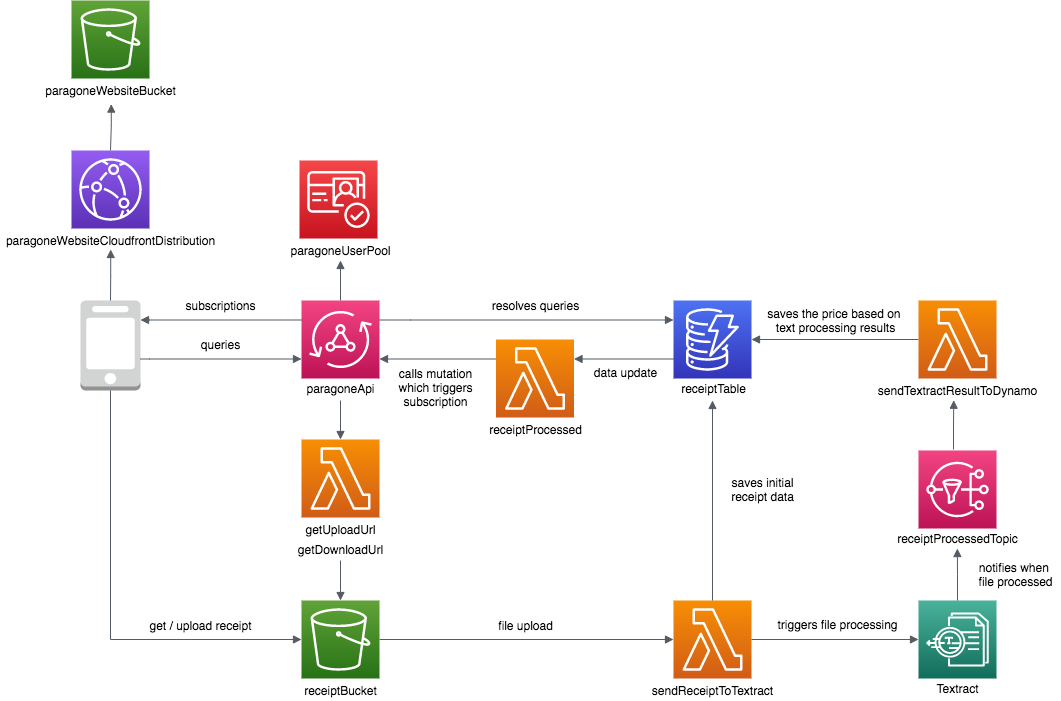
\includegraphics[width=1\textwidth]{assets/04-serverless-for-web-apps/paragoneArchitecture.png}
    \caption{Architecture of receipt processing web application}
    \label{fig:paragone-web-app}
\end{figure}

Key points of the suggested architecture:

\begin{itemize}
    \item \textbf{GraphQL as API} --- Presented example shows the basic backend of the web application built using the serverless technology. AWS AppSync is used to expose the GraphQL API, that is configured to trigger the AWS Lambda or communicate directly with some of the external services such as DynamoDB. Moreover, the integration with AWS Cognito introduces the authentication and authorization capabilities to the API. Each of the GraphQL operations, such as queries, mutations and subscriptions can be restricted, to ensure that only logged in users have access to their private data. Once the receipt processing is completed and the data is stored in the database, the user is notified in real-time about the results of the asynchronous operation, based on the established GraphQL subscription. The AWS Lambda, that is polling the DynamoDB for the event stream including inserts and updates for a given table, triggers the GraphQL mutation, which in turn pushes the new data to the client.
    \item \textbf{Secure and direct access to services storing the files} --- The GraphQL API, built on top of the AWS AppSync services, is not designed with intent to handle the operations on the files including downloads and uploads. Instead, the mechanism of presigned URLs is incorporated. It enables the client application to directly communicate with the Amazon S3 in a secure way, to access or store the files with predefined names and within a limited and strictly defined period of time. It alleviates the need of using the AWS Lambda to process and insert the data into the bucket upon the user request, which could be more time-consuming operation compared to generating the presigned URL.
    \item \textbf{Asynchronous receipt processing} --- The receipt processing flow is performed in an asynchronous manner, similarly to many other processing flows that utilise the serverless paradigm. Uploading the receipt to Amazon S3 triggers the AWS Lambda, which is responsible for inserting metadata about the image to the database and sending the receipt to Amazon Textract performing the document analysis task. Once the processing is completed, the Amazon SNS receives the event with the job identifier, which further triggers the AWS Lambda subscribing to the particular topic. The serverless function retrieves the data and based on simple heuristics, analyses the results of the text extraction process and stores the information further in DynamoDB.
    \item \textbf{Web application hosting} --- The backend of the application, composed from the combination of configured with each other services mentioned earlier, is effectively hosted in the cloud. Similarly, the client application once built, it can be stored in a publicly available Amazon S3 bucket in the form of the static assets. Amazon CloudFront distribution can be additionally integrated to provide the capabilities of Content Delivery Network, delivering the client application to users in a more convenient way.
\end{itemize}

Along with the simple heuristics retrieving the information based on the text extraction process, the more sophisticated services could be incorporated in the receipt processing flow, for example to categorise the products or services or provide more detailed spending statistics. Nevertheless, the other services would also operate in the same, asynchronous manner, extending the presented flow and performing the computation in a form of a distributed system composed of several components hosted in the cloud.

\subsubsection{Discussion}

The proposed solution presents the fully fledged web application built using the serverless architecture, including the serverless backend responsible for processing and storing the data along with the client application hosted in the cloud environment. 
The presented architecture is also a good ilustration of different execution models of the AWS Lambda, covered in more details in section \ref{chapter:lambda-function-execution-model}, including synchronous execution to obtain the presigned URL, composing of the asynchronous processing of the receipts as well as polling the stream of updates from the DynamoDB.

The asynchronous processing orchestration, described in more details in section \ref{chapter:serverless-processing-function-composition-and-orchestration}, is a common pattern in the serverless architecture and refers to composition of multiple components, responsible for particular chunks of the processing and forming effectively a distributed system.
The AWS Lambda is used to incorporate the business logic of the application, transforming the data when desired and using the other services to orchestrate the flow or handle the processing, without waiting idle for the results, but rather being triggered on a event-driven manner.

The use of Amazon Textract brings new development opportunities, allowing to integrate the service in the processing flow with convenient billing per usage and eliminates the need to maintain similar self-hosted service.

AWS AppSync serves as a feature-rich gateway of the application backend, triggering Lambda functions or directly communicating with other services to retrieve the data, but also allows to update the client in real-time using the subscriptions, which is a beneficial features for the asynchronous processing.
All of the processing is performed in a secure and compliant way, thanks to the authenticaton and authorization capabilities introduced by the integration of AWS AppSync with the Amazon Cognito, along with the presigned URL mechanism, enabling to safely store and retrieve the files from Amazon S3 bucket.

\subsection{Generating interactive slideshow based on LaTeX files} \label{chapter:examples-generating-interactive-slideshow-based-on-latex-files}

\subsubsection{Problem description}

The second example covers an implementation of web application similar to the Pitagoras Korepetytor\footnote{\url{http://pitagoras-korepetytor.pl/}}, which is a service playing a role of the virtual math tutor for high school students.
It provides a large collection of exercises, which can be further adjusted by the users when changing the values of the exercise parameters.
Based on the user input, the service generates an interactive slideshow, which is further previewed to the user using the interactive client application.
The slides present the following steps required to solve the exercise, with the additional audio commentary, explaining the performed mathematical operations.

\subsubsection{Proposed processing flow} \label{chapter:examples-generating-interactive-slideshow-based-on-latex-files-proposed-processing-flow}

When inspecting the processing results of the original solution, the user is given a set of slides along with the audio files, which are later processed by the presentation player on the client side.
Due to the large number of the parameters combinations that can be specified by the user and their value domains, generating the slides and commentary for all possible input values can occupy a lot of memory and be unprofitable.
Moreover, some of the presentations include advanced math equations, graphics visualising more sophisticated geometry problems or even considering some conditional logic based on parameters, upon which the solution for the exercise is generated.

Taking into consideration the problem and its requirements described above, the LaTeX \cite{latex} typesetting language and its processor is one of the possible solutions for the problem, which is well-known and frequently used in the academia community.
It enables the presentation creator to easily define the mathematical computations, present graphics showing the geometric tasks, which can be also extended based on the defined variables, including even some computations performed by the LaTeX processor or conditional logic.

Taking into account the selected tool, the processing flow for the user request could take the following:

\begin{enumerate}
   \item The initial step, taking place before the processing of the file is started, can be used to validate the user input. The entered values can be compared with the constraints of the exercise along with verifying if the user can preview the particular presentation, based on the business logic of the service.
   \item Once the input is verified and the user is allowed to request the presentation, the exercise variables from the input can be injected into the LaTeX file. 
   Next, the presentation is generated to the PDF file, which is further split into separate slides in the form of SVG files.
   \item Along with the slideshow generation, the initial presentation file can include additional directives with the commentary, which are extracted and supplemented with the variables from the user input. The processed text can be transformed further into the human-like audio commentary using the voice synthesis software.
   \item Additionally, some metadata about the presentation can be retrieved, including the slide durations for the slideshow or the information when to play the audio commentary, which will be sent and used later by the client application.
   \item The steps 2-4 can be performed in parallel. Once they are completed, the result can be afterwards sent to the client, previewing the slideshow with the exercise to the user.
\end{enumerate}

The described flow presents a rather extraordinary task incorporated in a web application, which plays a significant role in fulfilling the business logic of the proposed services.
In the traditional architecture, the responsibility of performing the presentation processing could be extracted into a separate service, that triggers one of the presentation processing worker based on the user requests.
With the limited traffic, the approach with a separate service communicating with a set of workers would be suitable, but when a larger group of users would submit the exercises to be processed within a short period of time, the scalability of such a system should require to scale the workers accordingly.
The instant scalability of the serverless architecture, with a pay-as-you-go billing model, would be beneficial to meet the variable demand of the presentation processing requests.
Moreover, the high-quality services hosted in the cloud, that are capable of performing the voice synthesis, could be integrated in the solution.
However, processing the LaTeX files using the serverless function is a non-standard type of computation task, which requires the function runtime to be properly enhanced to fulfill the task.

\subsubsection{Designed solution}

The designed solution presented in the diagram covers the presentation processing workflow along with the communication with the client application responsible for displaying the slideshow based on the generated data. 
The practical research focused on configuring the serverless function along with the processing optimisations of the described flow is presented in more detail in section \ref{chapter:latex-processing-optimisation}.

\begin{figure}[H]
   \centering
   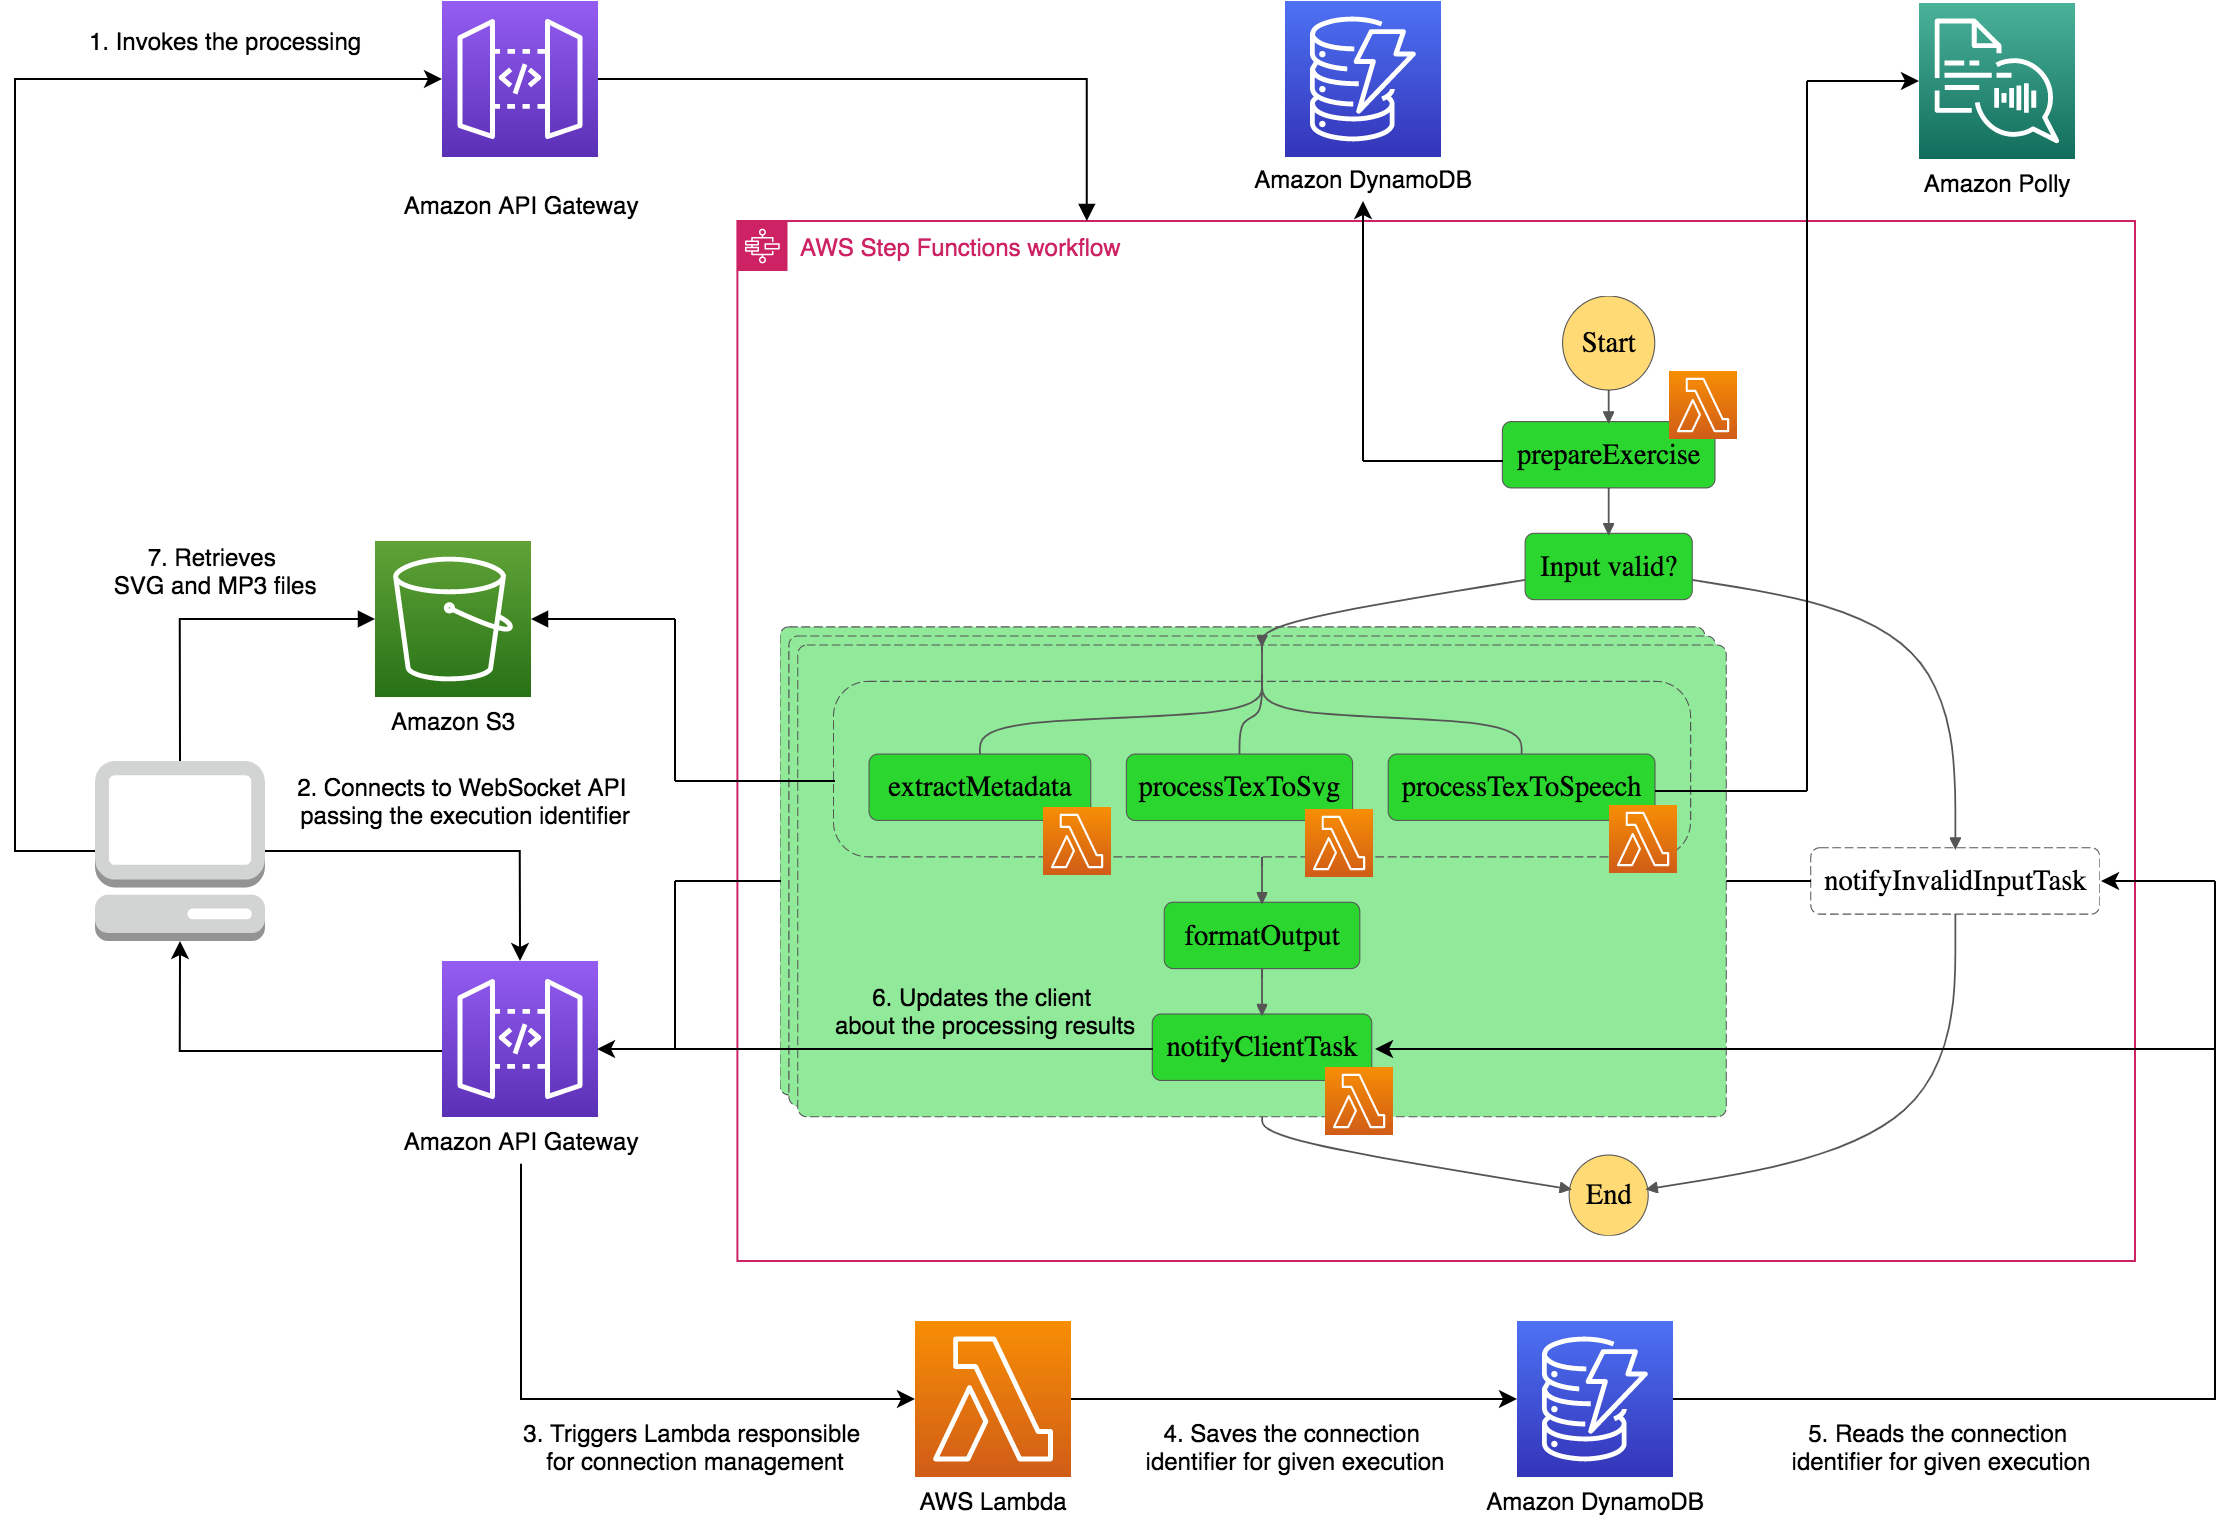
\includegraphics[width=1\textwidth]{assets/04-serverless-for-web-apps/euclidArchitecture.png}
   \caption{Architecture of presentation processing}
   \label{fig:euclid-web-app}
\end{figure}

Key points of the suggested architecture:

\begin{itemize}
   \item \textbf{Function orchestration using the AWS Step Function} --- The presentation processing flow is built on top of several AWS Lambda instances with the AWS Step Function orchestrating the whole process.
   AWS Lambda performs the initial task by retrieving the exercise details, validating the user input against the exercise constraints and defining the tasks for subsequent serverless function invocations, if the provided input satisfies the limitations.
   Based on the output of the first task, the further processing is executed or the user is notified about the invalid request.
   The presentation processing task is further separated into two chunks. 
   The first one generates the slideshow for several initial slides, which is pushed to the client as soon as possible once the processing is completed and starts previewing it to the user. While the second part, including the remaining chunk of the presentation, is delivered to the client later, when the user is busy watching the initial portion of the slideshow.
   For each of the chunks, three AWS Lambda instances are executed concurrently. They are responsible for processing the LaTeX file, extracting the slides in form of the SVG files that are later uploaded to the Amazon S3, generating the voice commentary using the Amazon Polly which are further stored in Amazon S3 as well as extracting some metadata about the generated slideshow.
   Once all three tasks for a given chunk are completed, the output of the functions is formated and another serverless function is invoked to push the results of the processing to the client using the WebSocket API
   \item \textbf{Pushing the update to the client} --- AWS Step Function orchestrates the processing in an asynchronous manner, which makes it necessary to notify the client once the processing is finished.
   Instead of using the polling techniques to periodically check whether the presentation is generated, the push based approach is used.
   Initially, the application client invokes the AWS Step Function and gets its execution ID.
   Next, it connects to the WebSocket API and sends a message with the obtained identifier, invoking the AWS Lambda that stores the execution ID along with the associated connection ID in the DynamoDB.
   When the chunk of the presentation is generated, the serverless function retrieves the data based on the execution ID and sends the message with the processing results to the associated client application.
   Finally, the slides and audio files, stored in the Amazon S3 bucket under predefined path, are retrieved.
\end{itemize}

\subsubsection{Discussion}

The proposed solution describes an interesting and non-standard use case of the serverless processing pipeline, responsible for preparing slideshow with the audio commentary based on the LaTeX files.
The predefined slideshows are requested by the user, making the desired outcome of the processing similar to the MindMup service, mentioned in section \ref{chapter:serverless-suitability-mindmup}.

The serverless architecture is an appealing technology for the file processing tasks, that are scheduled in an event-driven manner. 
The resource allocation based on demand along with autoscaling capabilities with proportional billing and scaling down to zero in absence of requests, makes the serverless technology an applicable and cost efficient solution to use.
However, the processing flow for the described example is more sophisticated and consits of several steps, which requires thoughtful coordination.
Moreover, the processing flow has been re-architectured across several subsequent steps to leverage the benefits of the serverless processing and make the slideshow processing more efficient.
The design process along with the preformance comparison and cost calculation for the given approach is presented in more details in section \ref{chapter:latex-processing-optimisation}.

The proposed solution relies on the orchestration of the processing that consits of the serverless function invocations, performing various tasks on different steps of the processing. 
AWS Step Function enables the processing to preserve state between the function execution along with orchestrating the flow to include some branching, tasks executed in parallel, mapping over list of tasks and gathering the results of the group of tasks.
The solution brings quite some elasticity when defining the processing schema and providing visualisation of the workflow, giving better insight into the executed processing.
However, the size of accumulated state in the AWS Step Function is strictly limited, which is insufficient to store the results of LaTeX files processing there, and required to use the Amazon S3 to preserve the processed files from different stages of the processing to make them later avaiable to the user.

Similarly to the previous example, the processing is performed in an asynchronous manner and requires some additional solution to update the client once the results are ready. The proposed solution invokes the AWS Step Function using the REST API and later connects via the WebSocket API to receive notification when the slideshow is available. 

Another challenge related with the proposed processing flow is related with the LaTeX files processing. The use of Lambda layer, including the additional dependencies, makes possible to perform such custom tasks and enhance the Lambda runtime with numerous capabilities.

Lastly, utilising the AWS Polly provided another development opportunity, which enabled to easily enhance the slideshow with the audio commentary, without the need to host similar service or incorporate some other third party service, running outside of the cloud platform.

\section{Server Tier}

\subsection{Lambda function as a compute resource}

The idea of Function as a Service has been already introduced in section \ref{chapter:serverless-faas}.
An example of such FaaS offering is AWS Lambda \cite{AWSLambda}, which is described as a compute service that require no resource management, it provides the auto-scaling capabilities, high-availability built-in and pay-per-use billing model, based on the function execution and the processing time with granularity of milliseconds. 

The following section analyses in more details the FaaS capabilities, considering the AWS Lambda as one of the implementations of this model, taking into account its limitations, runtime possibilities, execution models and possible optimisations.
Based on the overview of the AWS Lambda functionalities, the intuition of FaaS model capabilities as an execution environment can be established.

\subsubsection{Function limitations}

The AWS Lambda execution is constrained by quotas referring to the compute and storage resource that can be used by the serverless function.
Some of the AWS Lambda restrictions have been already discussed in section \ref{chapter:serverless-processing-limitations-runtime-and-data-restrictions}.
The list below includes additional limitations along with explanation of their impact on the processing of the serverless workloads \cite{AWSLambdaQuotas}.

\begin{itemize}
   \item \textbf{Concurrent executions} --- 1000 executions --- The serverless paradigm ensures about the infinite scalability of the underlying platform, however the default maximum number of functions that can be invoked is limited. It is essential to keep that in mind when developing some serverless solution extensively using the Lambda, that there is some threshold above which the function execution will be throttled. The limit can be increased further by the cloud provider.
   \item \textbf{Function memory allocation} --- from 128 MB to 10240 MB --- The function memory allocation can be configured, which translates into the available CPU and network bandwidth. When the memory of the function is set above the 1769 MB threshold, it provides processors with multiple cores capable of multithreading processing. Therefore, further increase for single threaded computation will increase the memory or bandwidth, which will be suitable accordingly for memory-bound or I/O-bound processing \cite{BecomeAServerlessBlackBelt}.
   \item \textbf{Function timeout} --- 900 seconds (15 minutes) --- The Lambda execution time is strictly limited, which makes it not suitable for processing various long-running tasks
   \item \textbf{Deployment package size} --- 50 MB (zipped) and 250 MB (unzipped, including layers) --- The function deployment package including the function code and its dependencies is constrained as well. The function execution environment can be additionally extended by the Lambda layers including additional code, libraries or dependencies. When the size constraints do not allow to pack all of the required dependencies, the function can be also based on the custom container image limited up to 10 GB. The topic of Lambda layer and container image is discussed further in section \ref{chapter:lambda-custom-runtimes}.
   \item \textbf{Invocation payload} --- 6 MB (synchronous invocation), 256 KB (asynchronous invocation) --- The invocation payload limit is related to the size of an event invoking the Lambda function.
   The synchronous invocation model requires the serverless function to return some value to the service triggering the function, for example the AWS API Gateway invoking the function based on user request, contrary to the asynchronous invocation, triggered for example by uploading some file to Amazon S3.
   The constraint prevents from passing large amounts of data in the event payload and requires the function to communicate with external components to retrieve or save the processing results if required.
   \item \textbf{Temporary directory storage} --- 512 MB --- Each of the invoked function environment is assigned a temporary storage, enabling the function to retrieve some data and perform the required processing in the local file system, which due to the ephemeral nature of the function containers, is further deprovisioned. The results of the processing need to be preserved in some dedicated storage component, depending on the type of the data being stored. Alternatively, under some circumstances, AWS Lambda can utilise the larger storage space when integrated with Amazon Elastic File System, which is a fully managed, shared file system service \cite{AWSLambdaEFS}.
\end{itemize}

\subsubsection{Function runtime} \label{chapter:lambda-custom-runtimes}

AWS Lambda supports natively several programming languages and their runtime environments including Node.js, Python, Java, C\#, Go and Ruby, with some of them including different versions of the runtime \cite{AWSLambdaRuntimes}. Most frequently the function code and its dependencies are compressed and packed by the deployment tool into a single zip archive and further stored by the cloud provider. When the Lambda function is invoked, the serverless platform allocates the resources to form the function environment, downloads the function code, bootstrap the language runtime with function dependencies and execute the function code. However, when the function has been recently triggered, the execution environment from a previous invocation can be reused, saving time required to prepare the environment and reusing some resources, such as established connections with external services or the temporary files.

Besides the standard function packing option and environment, the AWS Lambda enables to define Lambda layers, enabling to share dependencies independently, between several functions as well as custom container images.
Both of the approaches are described in more details below.

\paragraph{Lambda container image}

With the growth of containers popularity, it become a standard of the web application packing. The AWS Lambda allows to deploy the serverless functions based on custom Docker or OCI images, which enables developers to build serverless functions arbitrary from the supported programming languages and required dependencies \cite{AWSLambdaContainerImage}. Moreover, it allows to process other workloads depending on sizable dependencies, such as machine learning or other data intensive tasks.
Container images are constrained up to 10 GB in size, contrary to the aforementioned limit of the zipped function artifact, which make container images suitable to include custom runtimes, binaries and libraries, that can be used by the serverless function.
AWS provides a set of base images for supported runtimes as well as supported linux base image, however the developers can use any container image if it supports the Lambda Runtime API, which is a simple HTTP-based protocol, responsible for invoking the function and retrieving its results.
The custom container images can be built using familiar tooling and later uploaded to Amazon Elastic Container Registry, from which the image will be retrieved once the function is invoked.

Compared to other services enabling to run container based workloads, the Lambda container image support allows to scale workloads on per request basis and scale to zero with no additional cost if there is no traffic, providing more granular pricing model than other services. Moreover, the Lambda function is integrated with many AWS services, which means that it can be invoked from numerous event sources. 
Nevertheless, the Lambda still needs to satisfy the aforementioned limitations other than artifact size \cite{RunningContainerImagesInAWSLambda}.

\paragraph{Lambda layer}

When taking into consideration the encapsulated nature of the FaaS, several Lambda functions operating in the same part of the application logic can have some common methods, utilities and dependencies, effectively duplicating the same code in every deployed artifact.
Lambda layer is effectively a zip archive including additional code, dependencies and libraries, that can be shared across multiple Lambda functions, reducing the overall size of individual function artifacts.
When including the layer in a function, its content is extracted into function's local file system and can be further accessed by the function code, enabling functions to share common files and mitigating the problem of code duplication.
Moreover, the Lambda layer can include other, operating-system specific libraries and binaries used by the function code as well as custom runtimes, enabling developers to add required dependencies and execute code developed in any programming language in Lambda functions.
The function can include up to 5 layers, with the total size of the function code and layers summing up to 250 MB after decompressing \cite{AWSLambdaLayer}.

\subsubsection{Function execution} \label{chapter:lambda-function-execution-model}

The AWS Lambda is executed in an event-driven manner. 
The serverless function can be invoked by each of the defined triggers, configured based on the various event sources, including numerous services from the AWS cloud platform and their operations. 
The generic categorisation of data sources and invocation types for the serverless processing is described in section \ref{section:serverless-function-invocation}. 
AWS Lambda execution model fits into the mentioned classification and distinguish the following types of the function invocation \cite{OptimiseYourServerlessApplications}.
All of the mentioned execution models are present in the example implementation of the receipt processing application, mentioned in section \ref{chapter:examples-receipt-processing}.

\begin{itemize}
    \item \textbf{synchronous (push based)} --- Most frequently refers to the components acting as an API Gateway, invoking the Lambda based on the request and while the function completes the execution, it returns the results to the API Gateway, which passes back the response to the client.
    When Lambda fails during the event processing, the error is returned to the service calling the function.
    In case of the receipt processing application, the AWS AppSync invokes the Lambda functions in a synchronous manner, when user performs query to obtain the presigned URL.
    \item \textbf{asynchronous (event based)} --- Covers all cases in which the service makes a request to the Lambda function, which is consuming an event, but once the execution is completed it has no possibility to return the information to the event source. 
    When the processing fails, the function is retried two more times by default.
    After that the erroneous event can be placed in the Dead Letter Queue or it can be directed to other function, if configured.
    The Lambda function, triggered after the receipt is uploaded to S3 bucket as well as the other one, invoked based on the notification from SNS topic, are the examples of the asynchronous function invocation.
    \item \textbf{stream (poll based)} --- When assigning the stream based services as the data source, Lambda service runs a poller, that is watching for the messages and once they are available, the stream of events forming a batch, can be passed to the function via the asynchronous event.
    If the processing fails for some reason, the whole batch can be retried based on maximum record age or maximum retry attempts, the malformed data can be extracted from the rest of the shard and retried separately from the correctly processed events. When the retry limit is reached, the shard can be sent to the separate SQS queue or SNS topic.
    In the receipt processing application, the Lambda is polling the DynamoDB stream and based on received records, it is responsible for performing the mutation to push the update to the client.
\end{itemize}

\subsubsection{Function optimisations}

The Function as a Service model, heavily utilised in the serverless paradigm as a compute resource, at a first glance seems to be limited with the ability to configure the function and possibilities to optimise its execution, because the cloud provider takes responsibility for provisioning the resources and executing the function.
However, the thorough design of the application architecture along with the proper composition of the function code and its configuration, regarding the event sources and underlying resources, has a significant impact on the performance of the executed function, which transfers directly to the cost of execution.
The possible optimisations and configuration adjustment suggested by various practitioners for optimising the Lambda function execution and improving the configuration are discussed below.

\paragraph{Lambda execution}

In terms of the Lambda function execution, the improvement possibilities can be divided between the cloud provider and the developers implementing the solution. Taking into consideration the function lifecycle, resource allocation along with the downloading function code is handled by the cloud provider, however the size of deployed artifact can have an impact on the cold start duration. Furthermore, the architecture of the function code can have an impact on initialising the function runtime along with required dependencies as well as executing the function code itself.

\begin{itemize}
   \item \textbf{Concise function logic} --- Focusing on developing functions with single purpose and well defined responsibility enables to create leaner functions with fever dependencies, which results with a smaller package once bundled.
   On the contrary to the ''monolithic'' functions, that include some branching logic based on the invocation event to invoke the particular part of the application logic, which takes longer to initialise and can extend the cold start duration \cite{BecomeAServerlessBlackBelt}.
   \item \textbf{Reduce the function dependencies} --- Similarly to the previous point, the amount and size of dependencies transfers to the function initialisation time.
   Depending on the programming language, only selected modules or functions can be imported to incorporate only selected subcomponents of libraries or use techniques like treeshaking to remove unused parts of imported dependencies.
   It allows to obtain smaller function artifacts, with fewer dependencies impacting the function start and execution time \cite{OptimiseYourServerlessApplications}.
   \item \textbf{Use function to transform data, not to transport it} --- Instead of using the Lambda function to transport the data between services, some serverless components from the AWS offering can be integrated to transfer the data directly between each other.
   Similarly, when retrieving the data from external services to the serverless function, it is beneficial to request only the required data instead of performing additional filtering in the function code. It reduces the time, when the function is waiting for an I/O operation, for example when reading the data from DynamoDB or files from S3, that directly reduces the function execution cost \cite{BecomeAServerlessBlackBelt}.
   \item \textbf{Leverage container reuse} --- The conception of the serverless functions assumes that every function execution is stateless and should not rely on existing state from the previous execution.
   However, due to optimisations of the function executions, when the subsequent event triggers the function in a short time after the previous execution is finished, the container environment can be reused along with the initialised runtime and its dependencies.
   The prehandler logic can be used to initialise the connection with external services, such as databases or obtain secrets required in the function handler logic, that can be performed once per runtime initialisation instead of for every function execution.
   Similarly, the function global state can be used as a cache rarely-changing data or lazy-load variables and dependencies, reducing the work and processing time for subsequent invocations \cite{AWSLambdaPerformanceOptimization}.
\end{itemize}

\paragraph{Lambda configuration}

\begin{itemize}
   \item \textbf{Configure function resources intentionally} --- As mentioned before, for each function the amount of memory can be configured, which transforms proportionally to the CPU and network bandwidth configuration.
   Depending on the type of workloads, the function performance can benefit from additional memory for computation, using multiple cores for multithreading processing, when the memory is configured above the 1.8 GB threshold as well as from additional bandwidth for I/O bound processing.
   In terms of the cost the Lambda function is billed per function invocation and execution time, proportionally to the amount of configured memory.
   It is essential to consider, that the function can process the event faster when having more memory, while having similar cost as the function with lower memory configuration that takes longer to finish the processing.
   To better understand the function execution behaviour depending on configuration and take a data-driven approach the AWS Lambda Power Tuning can be used, which is an open-source tool invoking the AWS Step Function executing the function with a set of predefined configurations, measuring the execution time and its cost \cite{BecomeAServerlessBlackBelt}.
   \item \textbf{Select appropriate event sources} --- When configuring the event trigger for the function, it is beneficial to use the configuration options to discard the uninteresting events. For example the message filter for SNS can select only messages with desired payload to invoke the function, while S3 trigger can specify the action performed on the bucket as well as prefix and suffix for the object key, that can be used to trigger the function, based on operation for a file on particular path, filename or extension, if applicable \cite{BecomeAServerlessBlackBelt}.
\end{itemize}

\subsection{Serverless processing model}

rb:TBD

\subsubsection{Serverless microservices} 

Frontend - API - API Gateway, ALB, AppSync

Backend - if communicating with other services - go async - messaging services SNS (topics), SQS (queues), Kinesis (streams) and EventBridge(event buses)

% https://youtu.be/TOn0xhev0Uk
% https://d1.awsstatic.com/whitepapers/microservices-on-aws.pdf
% https://youtu.be/d9Jb1WKCLd8
% https://www.youtube.com/watch?v=8zysQqxgj0I - SNS, SQS

\subsubsection{Function composition and orchestration} \label{chapter:serverless-processing-function-composition-and-orchestration}

async compared to step function

% ref to examples - composition (receipt) and orchestration (latex)
% https://theburningmonk.com/2020/08/choreography-vs-orchestration-in-the-land-of-serverless/
% https://www.youtube.com/watch?v=rDSWHNdYx6E

\subsection{Case study - Generating interactive slideshow based on LaTeX files} \label{chapter:latex-processing-optimisation}

The following section describes in more details the optimisation process behind the second example implementation of the web application introduced in section \ref{chapter:examples-generating-interactive-slideshow-based-on-latex-files}.
The Step Function is used in the designed solution to coordinate the processing of several AWS Lambda instances that perform the processing of the individual stages in the entire flow.

In the presented research, the tests and measurements of the individual processing steps and their configurations are conducted based on the two examples of presentations prepared using the LaTeX typesetting system.
The sample presentations, described in more details below,  resemble the exercises which could be used in the mentioned service and characterise with different levels of complexity due to their content.

\begin{itemize}
   \item Exercise 1 --- Covers the 71 page long presentation that includes the solution derivation for the trigonometric equation.
   \item Exercise 2 --- Is more demanding and larger, 103 page long presentation. The first part describes the required steps for solving a geometry problem, with additional calculations included in the second part of the exercise.
\end{itemize}

From the initial research and experimenting with the possible solutions, the process of exporting the presentations to the PDF format has been identified as a bottleneck in the entire processing, taking significantly longer than the other steps performed in parallel.
The conducted performance tests consider mainly the processing duration from the client point of view, which is calculated as a time from requesting the invocation of Step Function, until the processing results are received by the client once the slideshow generation is completed and the assets are available in the S3 bucket.
Along with measuring the processing time, several other metrics have been gathered, giving more insight into the performance of individual steps of the processing.
Measurements preserve the preconditions listed below:

\begin{itemize}
   \item Each of the tests is performed 10 times and the presented results are the average of the conducted measurements.
   \item The cold start is ensured by re-deploying the infrastructure on the cloud environment and it is confirmed by the logs from the serverless function executions.
   \item The LaTeX files related to generating the presentation are removed from the temporal disc space of the function execution container once the processing is completed.
   The operation is performed to prevent a situation, when the subsequent function execution utilises the same instance of the serverless function and can benefit from the intermediate processing results from the previous invocation, which could affect the warm start execution results.
\end{itemize}

\subsubsection{Lambda container image and Lambda layer}

As mentioned before, generating of the presentation based on the LaTeX file can be classified as a custom type of processing for the serverless function runtime, that goes beyond the standard set of its tasks. The section \ref{chapter:lambda-custom-runtimes} discusses in more details the possibilities of the serverless platform in terms of performing such custom tasks. The following section presents the results of generating the PDF file with presentation using two approaches:

\begin{itemize}
   \item Container image --- uses the official Amazon container image for Node.js runtime with additional LaTeX distribution and other libraries required for the processing.
   \item Lambda layer --- includes the LaTeX distribution extracted from the aforementioned container image into the separate archive along with the additional Lambda layer including the Perl interpreter required for the file processing.
\end{itemize}

Both of the approaches execute the same function code running in the Node.js runtime, which uses the provided LaTeX distribution to generate the presentation.

\pgfplotstableread{
% xaxis1, xaxis2, Layer Cold, Layer Warm, Image Cold, Image Warm
0.225 0.275 5.455 2.147 7.943 2.209
0.725 0.775 9.469 5.235 10.832 5.210
}\datasetLayerVsImage

\begin{figure}[H]
    \begin{tikzpicture}
    \begin{axis}[ybar,
        width=.9\textwidth,
        ymin=0,
        ymax=12,        
        xmin=0,
        xmax=1,        
        ylabel={Response time [s]},
        bar width=4ex,
        xtick=data,
        xticklabels = {Exercise 1, Exercise 2},
        x tick label style={align=center,xshift=2ex},
        major x tick style = {opacity=0},
        minor tick length=1ex,
        legend style={at={(0.49,0.99)},anchor=north east},
        ]
            
    \addplot[draw=black,fill=blue!40,error bars/.cd,y dir=both,y explicit] 
        table[x index=0,y index=2] \datasetLayerVsImage; % Layer Cold
    \addplot[draw=black,fill=red!40,error bars/.cd,y dir=both,y explicit] 
        table[x index=0,y index=3] \datasetLayerVsImage; % Layer Warm
    \addplot[draw=black,fill=blue!70,error bars/.cd,y dir=both,y explicit] 
        table[x index=1,y index=4] \datasetLayerVsImage; % Image Cold
    \addplot[draw=black,fill=red!70,error bars/.cd,y dir=both,y explicit] 
        table[x index=1,y index=5] \datasetLayerVsImage; % Image Warm
    \legend{Lambda layer - cold start, Lambda layer - warm start, container image - cold start, container image - warm start}
    \end{axis}
    \end{tikzpicture}
    \caption{Response time comparison of the solutions using custom container image for AWS Lambda and Lambda layers with the LaTeX distribution}
    \label{chart:step-function-lambda-layer-vs-container-image}
\end{figure}

Key takeaways of the container image and Lambda layer processing comparison:

\begin{itemize}
    % rb: new
    \item Cold start times --- The significant processing time difference can be noticed when comparing the executions with cold and warm starts.
    The cold start time can be further divided into two parts. The first one considers the overhead related with the resource allocation from the large resource poll hosted by the cloud provider, downloading the function code and starting new, ephemeral container to execute the function.
    The second part is related to bootstrapping the function runtime as well as initialising dependencies required to execute the function handler.
    The detailed results of the cold start analysis are presented in the Table \ref{table:impact-of-the-cold-start-on-the-presentation-processing-task-for-approach-using-lambda-layer} and \ref{table:impact-of-the-cold-start-on-the-presentation-processing-task-for-approach-using-lambda-container-image}.

    \begin{table}[h]
        \centering
        \begin{tabular}{ |c|c|c|c|c|c| } 
        \hline
        Exercise & Execution & Function [ms] & Environment [ms] & Runtime [ms] & Execution [ms] \\
        \hline
        \multirow{2}{*}{Exercise 1} & cold start & 3609 & 914 & 273 & 2422 \\
        & warm start & 1614 & 34 & 0 & 1580 \\
        \hline
        \multirow{2}{*}{Exercise 2} & cold start & 7802 & 468 & 279 & 7055 \\
        & warm start & 4661 & 52 & 0 & 4609 \\
        \hline
        \end{tabular}
        \caption{Impact of the cold start on the presentation processing task for approach using Lambda layer}
        \label{table:impact-of-the-cold-start-on-the-presentation-processing-task-for-approach-using-lambda-layer}
    \end{table}

    \begin{table}[h]
        \centering
        \begin{tabular}{ |c|c|c|c|c|c| } 
        \hline
        Exercise & Execution & Function [ms] & Environment [ms] & Runtime [ms] & Execution [ms] \\
        \hline
        \multirow{2}{*}{Exercise 1} & cold start & 6548 & 637 & 1108 & 4803 \\
        & warm start & 1638 & 45 & 0 & 1593 \\
        \hline
        \multirow{2}{*}{Exercise 2} & cold start & 8945 & 316 & 810 & 7819 \\
        & warm start & 4614 & 35 & 0 & 4579 \\
        \hline
        \end{tabular}
        \caption{Impact of the cold start on the presentation processing task for approach using Lambda container image}
        \label{table:impact-of-the-cold-start-on-the-presentation-processing-task-for-approach-using-lambda-container-image}
    \end{table}

    The runtime initialisation time of the solution using Lambda layer is comparable for both exercises and it is equal on the average to 273 ms and 279 ms for Exercise 1 and Exercise 2 accordingly. 
    For the processing using the container image solution, the runtime initialisation time is on the average equal to 1108 ms and 810 ms, which has a visible impact on the overall processing time. Moreover, the cold start time of the solution based on the container image is additionally billed accordingly to AWS Lambda pricing, on the contrary to the approach using the Lambda layer in which the cold start time is not included into the cost.
    The processing performance evaluation of both approaches for the Exercise 1 preceeded the Exercise 2, which could explain the decrease of the time required to download the function code and allocate resources.
    \item Warm start times --- When considering the prewarmed function environments, there is no visible difference in the overall processing time between both of the tested solutions.
    \item Step Function overhead --- The orchestration overhead computed as the overall processing time of the Step Function decreased by the time of particular tasks defined in the Step Function flow, ranges from 400 ms and 450 ms, for both cold and warm starts.    
\end{itemize}

Based on the results of the comparison the Lambda layer is selected as a more suitable solution for further workflow optimisation.

\subsubsection{Function chain length}

In the previous section, the task of generating PDF presentations from the LaTeX files is discussed, however the flow proposed in section \ref{chapter:examples-generating-interactive-slideshow-based-on-latex-files-proposed-processing-flow} describes the additional step of extracting the individual slides from the presentation to SVG files. To achieve this, the lightweight \textit{pdf2svg} \cite{pdf2svg} library is used. The following scenario measures the processing performance in two configurations:

\begin{itemize}
   \item Single function --- the conversion is performed in a single function that generates the presentation and extracts the slides which are stored further in the S3 bucket.
   \item Function chain --- the processing is performed in the separate functions, storing the intermediate PDF file in the S3 bucket.
\end{itemize}

\pgfplotstableread{
% xaxis1, xaxis2, Single Cold, Single Warm, Chain Cold, Chain Warm
0.225 0.275 6.242 2.724 7.084 2.970
0.725 0.775 10.039 5.731 11.612 5.963
}\datasetChainVsSingle

\begin{figure}[H]
    \begin{tikzpicture}
    \begin{axis}[ybar,
        width=.9\textwidth,
        ymin=0,
        ymax=12,        
        xmin=0,
        xmax=1,        
        ylabel={Response time [s]},
        bar width=4ex,
        xtick=data,
        xticklabels = {Exercise 1, Exercise 2},
        x tick label style={align=center,xshift=2ex},
        major x tick style = {opacity=0},
        minor tick length=1ex,
        legend style={at={(0.465,0.99)},anchor=north east}
        ]

    \addplot[draw=black,fill=blue!40,error bars/.cd,y dir=both,y explicit] 
        table[x index=0,y index=2] \datasetChainVsSingle; % Single Cold
    \addplot[draw=black,fill=red!40,error bars/.cd,y dir=both,y explicit] 
        table[x index=0,y index=3] \datasetChainVsSingle; % Single Warm
    \addplot[draw=black,fill=blue!70,error bars/.cd,y dir=both,y explicit] 
        table[x index=1,y index=4] \datasetChainVsSingle; % Chain Cold
    \addplot[draw=black,fill=red!70,error bars/.cd,y dir=both,y explicit] 
        table[x index=1,y index=5] \datasetChainVsSingle; % Chain Warm
    \legend{Single function - cold start, Single function - warm start, Function chain - cold start, Function chain - warm start}
    \end{axis}
    \end{tikzpicture}
    \caption{Response time comparison of the solutions using single function and function chain to process the presentation}
    \label{chart:step-function-single-function-vs-function-chain}
\end{figure}

Key takeaways of the comparison:

\begin{itemize}
   \item Keep the function chain short --- When chaining several functions to perform some workflow, the overhead related to the communication and the cold start compounds. Additionally, the intermediate results need to be stored in some external component, which introduces additional work and latency that can be noticeable especially when working with large volumes of the data.
   \item Lambda layers constraints --- The small size of the \textit{pdf2svg} library makes it suitable for adding it and its dependencies to the Lambda layer, that include the LaTeX distribution already. However, it is crucial to take into account the limitations of the approach using the Lambda layers, described in more detail in section \ref{chapter:lambda-custom-runtimes}, because at some point it may be not possible to extend the function further.
\end{itemize}

\subsubsection{Parallel processing} \label{section:case-study-parallel-processing}

The serverless architecture is characterized by the capabilities of almost instant auto-scaling to meet the demand of the processing.
Some types of the processing can be re-designed to utilise such feature of the architecture and improve the overall processing time by parallelising the workload.
Generating the presentation in the PDF format from the LaTeX files is a custom type of processing task, that under some circumstances can be parallelised as well to certain degree.
The chosen slides from the presentation prepared using the Beamer package \cite{beamer} can be selected using the \textit{\textbackslash includeonlyframes} directive.
However, the presentation generation process requires to repeat some initial and common part of the processing regardless of the selected subset of slides, which causes some processing to be repeated for each of the presentation chunk.

The taken approach splits the LaTeX processing into several serverless function executions running in parallel. Each of the functions is assigned to generate the slides for predefined presentation chunks, containing 5 consecutive slides. Once the processing of all serverless functions is completed, along with the commentary transcription and metadata extraction, the user is notified about the results of the processing. The Step Function processing graph is presented in Figure \ref{fig:step-function-processing-the-presentation-in-parallel}, indicating that the presentation processing is divided into chunks, that are mapped to independent function calls.

\begin{figure}[H]
    \centering
    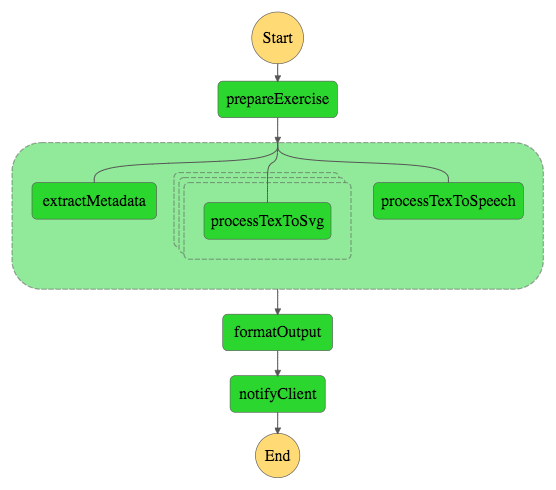
\includegraphics[width=0.6\textwidth]{assets/04-serverless-for-web-apps/stepFunctionGraphParallel.png}
    \caption{Step Function processing graph --- Generating the presentation chunks in parallel}
    \label{fig:step-function-processing-the-presentation-in-parallel}
\end{figure}

\pgfplotstableread{
% xaxis1, xaxis2, Single Cold, Single Warm, Parallel Cold, Parallel Warm
0.225 0.275 6.242 2.724 4.996 2.136
0.725 0.775 10.039 5.731 7.477 3.186
}\datasetSingleVsParallel

\begin{figure}[H]
    \begin{tikzpicture}
    \begin{axis}[ybar,
        width=.9\textwidth,
        ymin=0,
        ymax=12,        
        xmin=0,
        xmax=1,        
        ylabel={Response time [s]},
        bar width=4ex,
        xtick=data,
        xticklabels = {Exercise 1, Exercise 2},
        x tick label style={align=center,xshift=2ex},
        major x tick style = {opacity=0},
        minor tick length=1ex,
        legend style={at={(0.5175,0.99)},anchor=north east}
        ]

    \addplot[draw=black,fill=blue!40,error bars/.cd,y dir=both,y explicit] 
        table[x index=0,y index=2] \datasetSingleVsParallel; % Single Cold
    \addplot[draw=black,fill=red!40,error bars/.cd,y dir=both,y explicit] 
        table[x index=0,y index=3] \datasetSingleVsParallel; % Single Warm
    \addplot[draw=black,fill=blue!70,error bars/.cd,y dir=both,y explicit] 
        table[x index=1,y index=4] \datasetSingleVsParallel; % Parallel Cold
    \addplot[draw=black,fill=red!70,error bars/.cd,y dir=both,y explicit] 
        table[x index=1,y index=5] \datasetSingleVsParallel; % Parallel Warm
    \legend{Single function - cold start, Single function - warm start, Parallel processing - cold start, Parallel processing - warm start}
    \end{axis}
    \end{tikzpicture}
    \caption{Response time comparison of the solutions using single function to generate the complete presentation and the parallelised processing of separate chunks}
    \label{chart:step-function-single-function-vs-parallel-processing}
\end{figure}

Key takeaways of the parallel processing compared to the single function execution:

\begin{itemize}
    \item Parallelising the LaTeX files processing --- Even though the presentation generation processing cannot be effectively parallelised, the overall processing time is reduced for both of the provided examples.
   The complexity of the selected examples has a significant impact on the total processing time.
   When measuring and comparing the processing time on the local machine, generating the chunks independently for the Exercise 1 reduced the overall processing time by 32\%, while for the Exercise 2 it reached approximately 74\%.
  
   The average execution time for the presentation generation task of the chunks compared to the complete presentation is presented in Table \ref{table:overhead-of-the-presentation-processing-task-for-the-whole-presentation-and-chunks-including-5-slides}

    \begin{table}[h]
        \centering
        \begin{tabular}{ |c|c|c|c|c|c| } 
        \hline
        Exercise & Execution & Complete [ms] & Avg. of chunks [ms] & Time reduction [\%] \\
        \hline
        \multirow{2}{*}{Exercise 1} & cold start & 3349 & 2748 & 17.95 \\
        & warm start & 1641 & 1100 & 32.97 \\
        \hline
        \multirow{2}{*}{Exercise 2} & cold start & 7887 & 4310 & 45.35 \\
        & warm start & 4679 & 1313 & 71.94 \\
        \hline
        \end{tabular}
        \caption{Time reduction of the presentation processing task for the complete presentation and chunks including 5 slides}
        \label{table:overhead-of-the-presentation-processing-task-for-the-whole-presentation-and-chunks-including-5-slides}
    \end{table}

   \item Orchestrating parallel processing brings overhead --- It is essential to consider the additional overhead related to the orchestration of several serverless functions processing the presentation chunks in parallel. In the following example, the orchestration overhead is calculated as the Step Function duration decreased by the average tasks duration. It is equal to 873 ms (cold start) and 890 ms (warm start) for Exercise 1 as well as 1765 ms (cold start) and 1745 ms (warm start) for Exercise 2.
   \item Cost of the parallel processing --- Besides the processing overhead, the parallel execution brings additional cost for each of the executed serverless functions and its execution time. Moreover, for the given example the processing cannot be effectively parallelised and some part of the processing and retrieving the file is repeated for each invoked function.
\end{itemize}

\subsubsection{Updating the client with processed batches} \label{section:case-study-updating-the-client-with-processed-batch}

The approach presented in the previous section enables to effectively parallelise the processing and reduce the overall processing time, but it is restricted by the fact that all of the presentation chunks needs to be processed to push the update to the client. When taking into consideration how the presentations are prepared, most frequently the first several slides include the introduction to the exercise that usually takes more than 10 seconds. From the user perspective, only the first batch is required to start presenting the slideshow, while the remaining part of the assets can be delivered later.

The further improvements of the processing flow takes into account the aforementioned assumption and parallelises the presentation processing on the higher level, to deliver the updates of the processed presentation chunks independently. The Step Function processing graph of suggested approach is presented in Figure \ref{fig:step-function-pushing-updates-to-the-client-with-partially-processed-presentation}. The further measurements reflects the response time of two configurations of the flow described below:

\begin{itemize}
   \item First batch with 5 initial slides processed and the second batch with the remaining part of the presentation --- the processing is effectively parallelised in two branches.
   \item Each of the batches include information about 5 consecutive slides --- the processing is parallelised depending on the size of the presentation, with each of the branches processing 5 consecutive slides.
\end{itemize}

The results of the processing are compared with processing time of the complete presentation by a single serverless function and when the processing is parallelised as shown in the previous section. The results are presented in the figures \ref{chart:step-function-initial-batch} and \ref{chart:step-function-batches}.

\begin{figure}[H]
    \centering
    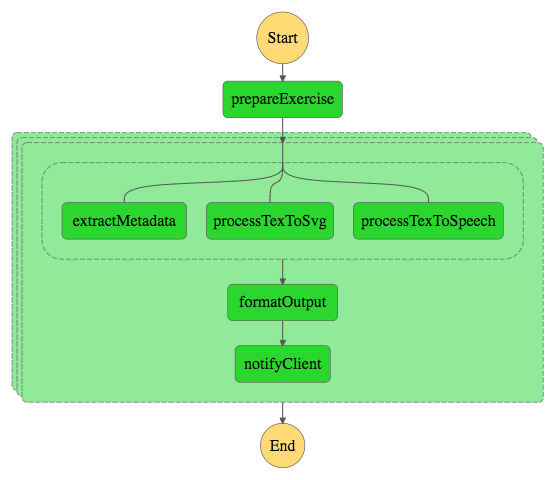
\includegraphics[width=0.6\textwidth]{assets/04-serverless-for-web-apps/stepFunctionGraphInitialBatch.png}
    \caption{Step Function processing graph --- Delivering updates to the client with processed presentation chunk}
    \label{fig:step-function-pushing-updates-to-the-client-with-partially-processed-presentation}
\end{figure}

\pgfplotstableread{
% xaxis, Single Cold, Single Warm, Parallel Cold, Parallel Warm, FirstBatch Cold, RestBatch Cold, FirstBatch Warm, RestBatch Warm
0.25 6.242 2.724 4.996 2.136 4.315 4.680 1.710 2.718
0.75 10.039 5.731 7.477 3.186 5.611 9.755 1.803 5.814
}\datasetUploadInitialBatch

\begin{figure}[H]
    \begin{tikzpicture}
    \begin{axis}[ybar,
        width=.9\textwidth,
        ymin=0,
        ymax=12,        
        xmin=0,
        xmax=1,
        bar width=3ex,  
        ylabel={Response time [s]},
        xtick=data,
        xticklabels = {Exercise 1,Exercise 2},
        major x tick style = {opacity=0},
        minor x tick num = 1,
        minor tick length=1ex,
        legend style={at={(0.5,0.99)},anchor=north east}
        ]
    \addplot[draw=black,fill=blue!40,error bars/.cd,y dir=both,y explicit] 
        table[x index=0,y index=1] \datasetUploadInitialBatch; % Single Cold
    \addplot[draw=black,fill=red!40,error bars/.cd,y dir=both,y explicit] 
        table[x index=0,y index=2] \datasetUploadInitialBatch; % Single Warm
    \addplot[draw=black,fill=blue!70,error bars/.cd,y dir=both,y explicit] 
        table[x index=0,y index=3] \datasetUploadInitialBatch; % Parallel Cold
    \addplot[draw=black,fill=red!70,error bars/.cd,y dir=both,y explicit] 
        table[x index=0,y index=4] \datasetUploadInitialBatch; % Parallel Warm
    \addplot[draw=black,fill=blueDark!50,error bars/.cd,y dir=both,y explicit] 
        table[x index=0,y index=5] \datasetUploadInitialBatch; % FirstBatch Cold
    \addplot[draw=black,fill=blueDark!80,error bars/.cd,y dir=both,y explicit] 
        table[x index=0,y index=6] \datasetUploadInitialBatch; % RestBatch Cold
    \addplot[draw=black,fill=redDark!50,error bars/.cd,y dir=both,y explicit] 
        table[x index=0,y index=7] \datasetUploadInitialBatch; % FirstBatch Warm
    \addplot[draw=black,fill=redDark!80,error bars/.cd,y dir=both,y explicit] 
        table[x index=0,y index=8] \datasetUploadInitialBatch; % RestBatch Warm
    \legend{Single function - cold start, Single function - warm start, Parallel execution - cold start, Parallel execution - warm start, First batch - cold start, Second batch - cold start, First batch - warm start, Second batch - warm start}
    \end{axis}
    \end{tikzpicture}
    \caption{Response time comparison of the solution delivering the update to the client in the first batch including initial 5 slides and the second batch with remaining data}
    \label{chart:step-function-initial-batch}
\end{figure}

\pgfplotstableread{
% xaxis, Single Cold, Single Warm, Parallel Cold, Parallel Warm, FirstBatch Cold, RestBatch Cold, FirstBatch Warm, RestBatch Warm
0.25 6.242 2.724 4.996 2.136 12.615 12.867 11.792 12.366
0.75 10.039 5.731 7.477 3.186 22.563 22.948 22.209 22.374
}\datasetUploadBatches

\begin{figure}[H]
    \begin{tikzpicture}
    \begin{axis}[ybar,
        width=.9\textwidth,
        ymin=0,
        ymax=24,        
        xmin=0,
        xmax=1,
        bar width=3ex,  
        ylabel={Response time [s]},
        xtick=data,
        xticklabels = {Exercise 1,Exercise 2},
        major x tick style = {opacity=0},
        minor x tick num = 1,
        minor tick length=1ex,
        legend style={at={(0.5,0.99)},anchor=north east}
        ]
    \addplot[draw=black,fill=blue!40,error bars/.cd,y dir=both,y explicit] 
        table[x index=0,y index=1] \datasetUploadBatches; % Single Cold
    \addplot[draw=black,fill=red!40,error bars/.cd,y dir=both,y explicit] 
        table[x index=0,y index=2] \datasetUploadBatches; % Single Warm
    \addplot[draw=black,fill=blue!70,error bars/.cd,y dir=both,y explicit] 
        table[x index=0,y index=3] \datasetUploadBatches; % Parallel Cold
    \addplot[draw=black,fill=red!70,error bars/.cd,y dir=both,y explicit] 
        table[x index=0,y index=4] \datasetUploadBatches; % Parallel Warm
    \addplot[draw=black,fill=blueDark!50,error bars/.cd,y dir=both,y explicit] 
        table[x index=0,y index=5] \datasetUploadBatches; % FirstBatch Cold
    \addplot[draw=black,fill=blueDark!80,error bars/.cd,y dir=both,y explicit] 
        table[x index=0,y index=6] \datasetUploadBatches; % RestBatch Cold
    \addplot[draw=black,fill=redDark!50,error bars/.cd,y dir=both,y explicit] 
        table[x index=0,y index=7] \datasetUploadBatches; % FirstBatch Warm
    \addplot[draw=black,fill=redDark!80,error bars/.cd,y dir=both,y explicit] 
        table[x index=0,y index=8] \datasetUploadBatches; % RestBatch Warm
    \legend{Single function - cold start, Single function - warm start, Parallel execution - cold start, Parallel execution - warm start, First batch - cold start, All batches - cold start, First batch - warm start, All batches - warm start}
    \end{axis}
    \end{tikzpicture}
    \caption{Response time comparison of the solution delivering the update to the client in the separate batches}
    \label{chart:step-function-batches}
\end{figure}

Key takeaways of the proposed approach:

\begin{itemize}
   \item Improved response time of the initial batch --- For the first of the considered configurations, with the results presented in Figure \ref{chart:step-function-initial-batch}, the response time for the initial batch including the first slides is shorter.
   Once it is received by the client, the user can start previewing the slideshow, while the second batch including the remaining data can be processed and received by the client later.
   Such a solution enables the user to start previewing the exercise quicker, while the processing time of the complete presentation is hidden from the user perspective.
   \item Increase of the Step Function overhead for the fine-grained workflow coordination --- In the second configuration that parallelises the chunk processing and splits it into more branches, the overhead of the Step Function responsible for the orchestration makes the processing significantly longer.
   Moreover, the batch including 5 initial slides is frequently delivered as one of the last parts, significantly postponing the time when the user can start previewing the exercise as it is presented in the Figure \ref{chart:step-function-batches}.
\end{itemize}

\subsubsection{Comparing serverless solution with the traditional architecture}

When deciding on the serverless architecture, there is always a question how the solution will perform compared to the solution implemented using the more traditional architectures.
To answer that question for the given problem, a similar service based on a simple server running within the container has been created and hosted on the AWS Fargate. 
The server is executed in the Node.js runtime, similarly to the serverless functions from the previous steps of the study.
Moreover, it is reusing a significant part of the logic responsible for the initial validation of the task, processing the LaTeX presentation to PDF and then extracting separate slides to the SVG files, using the same libraries as well as uploading the results to S3 once the processing is completed.
The container is configured with the same amount of memory and CPU as the serverless function used for the processing in the serverless implementation.

The figure \ref{chart:step-function-compared-with-traditional-architecture} presents how the solution using the traditional architecture performs compared with the various configurations of the serverless solution.

\pgfplotstableread{
% xaxis, Single Cold, Single Warm, Parallel Cold, Parallel Warm, FirstBatch Cold, RestBatch Cold, FirstBatch Warm, RestBatch Warm
0.25 6.242 2.724 4.996 2.136 4.315 4.680 1.710 2.718 2.636
0.75 10.039 5.731 7.477 3.186 5.611 9.755 1.803 5.814 6
}\datasetCompareContainer

\begin{figure}[H]
    \begin{tikzpicture}
    \begin{axis}[ybar,
        width=.9\textwidth,
        ymin=0,
        ymax=12,        
        xmin=0,
        xmax=1,
        bar width=3ex,  
        ylabel={Response time [s]},
        xtick=data,
        xticklabels = {Exercise 1,Exercise 2},
        major x tick style = {opacity=0},
        minor x tick num = 1,
        minor tick length=1ex,
        legend style={at={(0.5,0.99)},anchor=north east}
        ]
    \addplot[draw=black,fill=blue!40,error bars/.cd,y dir=both,y explicit] 
        table[x index=0,y index=1] \datasetCompareContainer; % Single Cold
    \addplot[draw=black,fill=red!40,error bars/.cd,y dir=both,y explicit] 
        table[x index=0,y index=2] \datasetCompareContainer; % Single Warm
    \addplot[draw=black,fill=blue!70,error bars/.cd,y dir=both,y explicit] 
        table[x index=0,y index=3] \datasetCompareContainer; % Parallel Cold
    \addplot[draw=black,fill=red!70,error bars/.cd,y dir=both,y explicit] 
        table[x index=0,y index=4] \datasetCompareContainer; % Parallel Warm
    \addplot[draw=black,fill=blueDark!50,error bars/.cd,y dir=both,y explicit] 
        table[x index=0,y index=5] \datasetCompareContainer; % FirstBatch Cold
    \addplot[draw=black,fill=blueDark!80,error bars/.cd,y dir=both,y explicit] 
        table[x index=0,y index=6] \datasetCompareContainer; % RestBatch Cold
    \addplot[draw=black,fill=redDark!50,error bars/.cd,y dir=both,y explicit] 
        table[x index=0,y index=7] \datasetCompareContainer; % FirstBatch Warm
    \addplot[draw=black,fill=redDark!80,error bars/.cd,y dir=both,y explicit] 
        table[x index=0,y index=8] \datasetCompareContainer; % RestBatch Warm
    \addplot[draw=black,fill=green!60,error bars/.cd,y dir=both,y explicit] 
        table[x index=0,y index=9] \datasetCompareContainer; % RestBatch Warm
    \legend{Single function - cold start, Single function - warm start, Parallel execution - cold start, Parallel execution - warm start, First batch - cold start, Second batch - cold start, First batch - warm start, Second batch - warm start, Container environment}
    \end{axis}
    \end{tikzpicture}
    \caption{Response time comparison of the solutions using the serverless and traditional architectures}
    \label{chart:step-function-compared-with-traditional-architecture}
\end{figure}

Key takeaways of the serverless implementation comparison with the solution using the simple, containerized server application:

\begin{itemize}
   \item The performance of serverless implementation is comparable, when it is not affected by the cold starts --- The initial serverless solution orchestrating the flow and using single function to process the LaTeX file performs comparable when executed with warm start to the solution using the simple server hosted by AWS Fargate in the container. However, when the execution is affected by the cold starts, the response time is significantly longer as presented in Figure \ref{chart:step-function-compared-with-traditional-architecture}.
   It is beneficial to consider the interest in the service as well as the traffic pattern to estimate how often such a phenomenon may take place, when deciding on architecture selection or mitigating the negative influence by pre-warming the containers programmatically or by the service such as Provisioned Concurrency for AWS Lambda.
   % rb: new
   \item Re-designing the serverless processing to utilise its benefits can improve performance --- The presented configurations of the serverless solution confirms that remodeling the processing to use the benefits of the serverless paradigm can bring visible benefits in terms of the performance, compared to the solution using the more traditional architecture.
   However, some aspects and tasks of the proposed flow are required for the serverless solution, such as uploading the results of processing to S3, which could be further accessed by the user.
   The solution using the server could aggregate the results of processing locally, without the need to communicate with external component to store the files and return the results directly to the user, reducing the amount of work and cost.
   % rb: new
   \item Built-in scalability of the serverless architecture --- One of the features of the serverless architecture is the possibility of almost instant and effortless processing parallelisation, that reduces the overall processing time in that case.
   Further research could investigate in more details, how the implementations using both of the architectures are performing under the load resembling the behaviour of the potential users of the system.
   When considering the serverless solution, the impact could be visible by increased number of cold starts when the traffic pattern is changing or it is occasional. However, the solution using the simple server hosted in the container could note the performance decline similarly, when many subsequent requests would be submitted to a single worker instance or when the cluster of workers would need to scale to meet the demand.
\end{itemize}

rb: todo - scaling serverless - worst case cold start - running for cold starts running in parallel - resembling the behaviour of real users

\subsubsection{Cost of the designed solution}

Another, frequently mentioned factor when deciding on the architecture choice is the maintenance and execution cost. The serverless architecture makes it more difficult to precisely measure the cost of the processing due to the number of components and the variety of granularity in billing for used services. However then cost can be effectively estimated, when the traffic pattern is known along with the execution cost of particular workflow.

The section calculates the cost of a single execution of the entire processing flow for Exercise 1 considered in 2 configurations:

\begin{itemize}
   \item The parallel presentation processing describes in section \ref{section:case-study-parallel-processing}.
   \item The first configuration described in section \ref{section:case-study-updating-the-client-with-processed-batch}, in which the presentation processing is divided into two branches --- first with initial slides and the second with remaining data for the slideshow completeness.
\end{itemize}

The cost of services used in the implementations for Europe (Frankfurt) region and excluding the Free Tier is summarised in Table \ref{table:case-study-service-spendings-summary}. Cost of some of the services, such as Amazon CloudWatch for storing logs, API Gateway for the incoming traffic in form of the user requests or data transfer for DynamoDB is omitted due to negligible use and too little granularity of the included values in the cost statement.

\begin{table}[H]
    \centering
    \begin{tabular}{ |c|c|c| } 
    \hline
    Service & Billed service usage & Pricing \\
    \hline
    \multirow{3}{*}{API Gateway} & REST API - API Calls & \$3.70 (per million) \\ 
    & WebSocket API - Connection Minutes & \$0.285 per million connection minutes \\ 
    & WebSocket API - Message Transfers & \$1.14 (per million) \\ 
    \hline
    Data Transfer & From Amazon S3 To Internet & \$0.09 per GB \\
    \hline
    \multirow{2}{*}{DynamoDB} & Read request & \$0.305 per million read request units \\
    & Write request & \$1.525 per million write request units \\
    \hline
    \multirow{2}{*}{AWS Lambda} & Duration & \$0.0000166667 for every GB-second \\
    & Requests & \$0.20 per 1M requests \\
    \hline
    Polly & Standard voices & \$4.00 per 1 million characters \\
    \hline
    \multirow{2}{*}{Simple Storage Service} & PUT, COPY, POST, LIST requests & \$0.0054 (per 1,000 requests) \\
    & GET, SELECT, and all other request & \$0.00043 (per 1,000 requests) \\
    \hline
    Step Function & State transtition & \$0.025 per 1,000 state transitions\\
    \hline
    \end{tabular}
    \caption{Pricing summary for services used in the implementations}
    \label{table:case-study-service-spendings-summary}
\end{table}

The usage of the services for both implementations and their cost is summarised in Table \ref{table:case-study-service-parallel-spending-summary} and \ref{table:case-study-service-initial-batch-spending-summary}.

\begin{table}[H]
    \centering
    \begin{tabular}{ |c|c|c| } 
    \hline
    Service usage & Usage & Cost [\$] \\
    \hline
    REST API - API Calls & 2 requests & 0,0000074 \\
    WebSocket API - Connection Minutes & 2 minutes & 0,00000057 \\
    WebSocket API - Message Transfers & 4 messages & 0,00000456 \\
    \hline
    Data Transfer From Amazon S3 To Internet & 0.003 GB & 0,00027 \\
    \hline
    DynamoDB Read request & 1 Read Request Unit & 0,0000000305 \\
    DynamoDB Write request & 2 Write Request Unit & 0,0000000305 \\
    \hline
    AWS Lambda - Duration & 61.057 GB-second & 0,00102 \\
    AWS Lambda - Requests & 22 requests & 0,0000044 \\
    \hline
    Amazon Polly - Standard voices & 1323 characters & 0,00529 \\
    \hline
    S3 PUT, COPY, POST, LIST requests & 86 requests & 0,000464 \\
    S3 GET, SELECT, and all other request & 108 requests & 0,0000464 \\
    \hline
    Step Function - state transitions & 24 transitions & 0,0006 \\
    \hline
    \multicolumn{1}{c|}{} & \textbf{Total} & 0,00771 \\
    \cline{2-3}
    \end{tabular}
    \caption{Cost summary for the approach using parallel presentation processing}
    \label{table:case-study-service-parallel-spending-summary}
\end{table}

\begin{table}[H]
    \centering
    \begin{tabular}{ |c|c|c| } 
    \hline
    Service usage & Usage & Cost [\$] \\
    \hline
    REST API - API Calls & 2 requests & 0,0000074 \\
    WebSocket API - Connection Minutes & 4 minutes & 0,00000114 \\
    WebSocket API - Message Transfers & 5 messages & 0,0000057 \\
    \hline
    Data Transfer From Amazon S3 To Internet & 0.003 GB & 0,00027 \\
    \hline
    DynamoDB Read request & 1,5 Read Request Unit & 0,0000000456 \\
    DynamoDB Write request & 2 Write Request Unit & 0,0000000305 \\
    \hline
    AWS Lambda - Duration & 11.649 GB-second & 0,000194 \\
    AWS Lambda - Requests & 12 requests & 0,0000024 \\
    \hline
    Amazon Polly - Standard voices & 1323 characters & 0,00529 \\
    \hline
    S3 PUT, COPY, POST, LIST requests & 86 requests & 0,000464 \\
    S3 GET, SELECT, and all other request & 98 requests & 0,0000421 \\
    \hline
    Step Function - state transitions & 17 transitions & 0,000425 \\
    \hline
    \multicolumn{1}{c|}{} & \textbf{Total} & 0,00671 \\
    \cline{2-3}
    \end{tabular}
    \caption{Cost summary for the approach delivering the update to the client in the separate batches}
    \label{table:case-study-service-initial-batch-spending-summary}
\end{table}

% rb: new
Takeaways of the cost summary of designed solutions:

\begin{itemize}
   \item AWS Lambda processing is a small fraction of overall cost --- Cost summaries for both of the presented solutions indicate that the text-to-voice transcoding service takes a significant amount of the overall cost.
   The usage of the AWS Lambda processing is greater for the solution using parallel processing.
   Even though some part of the presentation processing is repeated in the serverless functions executed in parallel, the overall cost of the AWS Lambda related services barely exceeds 0.001\$ for the analysed example per single execution.
   Moreover, it is crucial to consider the cost of other services incorporated in the processing as well as the data transfer.
   For example, the summary of the second configuration indicates that the cost of uploading results to Amazon S3 and transferring them to the client exceeded the cost of the processing of the AWS Lambda.
   \item Serverless pay-per-use billing model --- Considering the Exercise 2 which is a more demanding task in terms of the processing and the summaries listed above, the overall cost of the processing for a single presentation could be estimated as not exceeding 0.01\$ per execution.
   Moreover, when taking into account the benefits of the serverless architecture, such as auto-scaling with granular billing model per usage and without paying for idle as well as the fact that the need for managing the infrastructure is handled by the cloud provider, the serverless solution with pay-per-use pricing can be an appealing alternative to more traditional architectures.
\end{itemize}

% Step Function 
% - map task - https://youtu.be/w6cqUhSdy-M
% - local dev - https://youtu.be/lKbeBBV1gyc?t=1996
% - architecturing serverless parallel computing - https://livebook.manning.com/book/serverless-architectures-on-aws-second-edition/chapter-8/v-7/1
% - https://serverlessland.com/patterns

\section{Data Tier}

\subsection{Issues when integrating traditional databases with serverless}

\subsection{Serverless databases}

% https://youtu.be/hwnNbLXN4vA
% https://thenewstack.io/what-front-end-developers-need-to-know-about-serverless-databases/
% https://www.alexdebrie.com/posts/dynamodb-no-bad-queries/
% https://www.alexdebrie.com/posts/dynamodb-patterns-serverless/

DynamoDB - modeling for cost optimisation, increase performance, single table design

Aurora

S3

how they work? streams, handling reusing connections, RDS proxy

\section{Client Tier}

\subsection{Client communication patterns for serverless architecture}

% https://youtu.be/yfJZc3sJZ8E - Gateway
% https://serialized.net/2020/09/multiplayer/ - WebSocket applicability
% https://youtu.be/XVU4pYeNfNo - AppSync
% https://hackernoon.com/using-protocol-buffers-with-api-gateway-and-aws-lambda-22c3804f3e76 - Protobufs

APIGateway - REST + websockets

AppSync - GraphQL - data aggregation from different resources

gatekeeper - authentication

direct resolvers to particular services with/without the lambda, pipeline resolvers (nested nodes in graph) - overhead comparison

calling the services from the client - presigned URLs / using client libs to have access to resources

\subsection{Serverless push based approach}

% https://aws.amazon.com/blogs/compute/from-poll-to-push-transform-apis-using-amazon-api-gateway-rest-apis-and-websockets/

request - response

poll to push pattern

GraphQL subscriptions triggered by mutation

\subsection{Hosting web clients}

hosting static files

server side rendering

\subsection{Thick and thin client}

% how serverless affects thicker/thinner client
% direct access to service


\backmatter

\bibliographystyle{amsalpha}{\raggedright\sloppy\small\bibliography{bibliography}}

\end{document}